\documentclass[11pt,twoside]{article}

\usepackage{
  amsmath,
  amssymb,
  amsthm,
  extarrows,
  fancyhdr,
  fullpage,
  graphicx,
  hyperref,
  mathrsfs,
  mathtools,
  microtype,
  sagetex,
  stmaryrd,
  tikz-cd,
  thmtools
}
\usepackage[nottoc]{tocbibind}
\usepackage{arith-curve}
\usepackage[
  paperwidth=5.4in,
  paperheight=8.675in,
  textwidth=5.125in,
  textheight=8in,
  centering
]{geometry}
\usepackage[all]{xy}
\hypersetup{
  colorlinks=true,
  linkcolor=blue,
  urlcolor=cyan
}
\pagestyle{fancy}
\fancyhf{}
\setlength{\headheight}{14pt}
\fancyhead[CE]{Arithmetic of curves}
\fancyhead[CO]{D.~Miller, D.~Zywina}
\fancyhead[RE]{\thepage}
\fancyhead[LO]{\thepage}

\title{Arithmetic of curves}
\author{Daniel Miller and David Zywina}
\date{Fall 2013}

\begin{document}
\maketitle
\tableofcontents





% !TEX root = 7390-notes.tex


\section{Introduction}


\subsection{Disclaimer}

These notes originated in a course ``Topics in algebra: the arithmetic of 
curves'' taught by David Zywina at Cornell University. However, a significant 
amount of material (including, no 
doubt, many errors) has been added since then, so they are far from an exact 
reflection of what he covered in class. Moreover, the notation has been changed 
in many places (sometimes significantly) as has the order in which material is 
covered. Most significantly, the tone of these notes differs drastically 
from the perspective Zywina took in class, with the notes being much more 
cohomological and scheme-theoretic than Zywina's generally elementary (and 
pedagogically correct) approach. Any errors in these notes are entirely the 
fault of the former author. 

The original computations were done using the commercial 
computer algebra system Magma. For these notes, everything has been reworked 
into Sage, an open-source alternative designed for for number theorists. Nearly 
all of the Sage code used is contained (using the \LaTeX{} package 
\texttt{sagetex}) in the source code for this document, which may be found at 
\url{https://github.com/dkmiller/arith-curve}. 





\subsection{Notation and conventions}

Following Bourbaki, we write $\dN$, $\dZ$, $\dQ$\ldots for the natural 
numbers, integers, \ldots. 

A \emph{nice variety} over a field $k$ is a smooth, projective, geometrically 
integral variety over $k$. 

If $k$ is a field, $k^s$ (resp.~$\bar k$) denotes its separable 
(resp.~algebraic) closure. We will write $G_k = \gal(k^s/k)$ for the 
\emph{absolute Galois group} of $k$. 

Let $X$ be a scheme over a finite field $\dF_q$. The \emph{Frobenius of $X$} 
is the morphism $\geomfrob_X:X\to X$ that is the identity on the underlying 
topological space, and $x\mapsto x^q$ on the structure sheaf. The Frobenius in 
$G_{\dF_q} = \gal(\overline{\dF_q}/\dF_q)$ is the \emph{arithmetic} Frobenius, 
induced by $x\mapsto x^q$ on $\overline{\dF_q}$. We will write $\arithfrob_q$ for 
the arithmetic Frobenius. 

If $v$ is a finite place of a global field $k$, then $k_v$ denotes the 
completion of $k$ with respect to $v$. Most of our notation here is standard, 
with the exception of $\kappa_v=\fo_v/\fp_v$ for the residue field of $v$. 

If $k$ is a global field and $v$ is a finite place of $k$, $\arithfrob_v$ denotes the 
arithmetic Frobenius associated to $v$. We will sometimes take $\arithfrob_v$ to be 
a single (non-canonical) element of $G_k$, or the elements' entire conjugacy 
class. This should not cause any confusion. 

If $E$ is a module over a ring $A$ and $x\in E$, then we will write $E/x$ 
instead of $E/(A\cdot x)$. In particular, for $a\in A$, $A/a$ is the quotient 
of $A$ by the ideal generated by $A$. 

All abelian groups are tacitly taken to modules over $\dZ$, so the previous 
convention applies. Even if an abelian group $G$ is written multiplicatively, 
$G/n$ will be used to denote $G/(G^n)$. We write $\torsion n G$ for the 
group $\{g\in G:n\cdot G=0\}$. 

The end of an example is marked by a triangle $\triangleright$. Following 
Bourbaki, we mark sections and paragraphs covering especially advanced 
material with a star $\star$. 










\subsection{Motivation: plane curves}



Fir a non-constant polynomial $f(x,y)\in\dQ[x,y]$. Assume $f$ is 
geometrically irreducible, that is, irreducible in the ring 
$\overline{\dQ}[x,y]$. We can define the curve $C$ over $\dQ$ determined by the 
equation $f(x,y)=0$. For now, we will think of $C$ in terms of its functor of 
points. To any $\dQ$-algebra $A$, we set $C(A)=\{(a,b)\in A^2:f(a,b)=0\}$. 
As a scheme, $C=\spec\left(\dQ[x,y]/f\right)$. Some big questions are:
\begin{enumerate}
  \item Is $C(\dQ)=\varnothing$?
  \item Is $C(\dQ)$ finite?
  \item Can we compute $C(\dQ)$?
\end{enumerate}
None of these questions can be answered in full generality. 

\begin{example}
Let $f=x^2+y^2-1$, i.e. $C$ is the circle. It is well-known that 
\[
  C(\dQ)=\left\{\left(\frac{1-t^2}{1+t^2},\frac{2t}{1+t^2}\right):t\in\dQ\right\}\cup \{(-1,0)\}
\]
This can be proved in the usual manner by choosing the point $(-1,0)$ in $C$, 
and then drawing lines with rational slopes through $(-1,0)$. As a Riemann 
surface, $C(\dC)$ is a sphere with two points removed. 
\end{example}

\begin{example}
Let $f=x^2+y^2+1$. Then $C(\dR)=\varnothing$, hence $C(\dQ)=\varnothing$. But 
as a Riemann surface, $C(\dC)$ is the same sphere with two points removed. Thus 
the geometry of $C$ does not necessarily determine $C(\dQ)$. 
\end{example}

\begin{example}
Let $f=x^4+y^4-1$. Then it is a theorem of Fermat that 
$C(\dQ)=\{(\pm 1,0),(0,\pm 1)\}$. It is a (much harder) theorem of Wiles that if 
$C_n$ is the curve given by $f=x^n+y^n-1$ for $n\geqslant 3$, then 
$C_n(\dQ)=\{(\pm 1,0),(0,\pm 1)\}$. In fact, this is the celebrated 
``Fermat's last theorem,'' proved in \cite{wi95}. 
\end{example}

\begin{example}[Stoll]
Consider 
\begin{align*}
  C : y^2 = 82342800 x^6 &- 470135160 x^5 + 52485681 x^4 + 2396040466 x^3 \\
    &+ 567207969 x^2 - 985905640 x + 247747600 \text{.}
\end{align*}
This is a curve of genus 2, i.e. $C(\dC)$ is a punctured two-holed 
torus. It turns out that $\# C(\dQ)\geqslant 642$ \cite[\S 6]{st09}. 
However, by a theorem of Faltings, $\# C(\dQ)$ is finite. This example exhibits 
the largest known number of rational points of a genus two curve 
over $\dQ$. If we take $C:y^2=f(x)$ with $f\in\dQ[x]$ a 
``random'' sextic polynomial, then the expectation is that 
$C(\dQ)=\varnothing$. 
\end{example}

It is natural to ask whether for each $g\geqslant 2$ there exists a number 
$B_g$ such that whenever a curve $C$ over $\dQ$ has genus $g$, we have 
$\# C(\dQ)\leqslant B_g$. This is not even known for $g=2$. 

\begin{example}
Let $C:y^2=x^3+875 x$. Note that $C(\dQ)$ has the obvious point 
$(0,0)$, and one can do a bit of work to show that this is the only point. 
\end{example}

\begin{example}
Let $C:y^2=x^3+877 x$. Then $C(\dQ)$ once again contains $(0,0)$. A 
computer search showed that $(0,0)$ is the only point on $C$ of height 
$\leqslant 1000000$. For now, the \emph{height} of a solution is just the 
largest absolute value of the numerator / denominator of a solution written 
in reduced fractions. But other methods lead us to expect many more solutions
(infinitely many, in fact). Let $E$ be the projective curve over $\dQ$ obtained 
by adjoining a point $O$ to $C$. As a Riemann surface, $E(\dC)$ is just a 
torus. 

We can give $E$ the 
structure of an \emph{abelian variety} over $\dQ$. That is, we can give $E$ the 
structure of a commutative algebraic group (the multiplication operation 
$m:E\times E\to E$ is given by regular functions), 
with $O$ being the identity. Later, we will think of $E$ as 
being identified with its jacobian $\jac(E)$ via the choice of a single point 
$O\in E(\dQ)$. Since $E$ is a commutative algebraic group, $E(\dQ)$ is an 
abelian group (with identity $O$). It is a theorem of Mordell that $E(\dQ)$ is 
finitely generated. We know the structure of such groups: 
$E(\dQ)\simeq A\times \dZ^r$, where $A$ is finite, and $r=\rank E$ 
is the \emph{(algebraic) rank} of $E$. 

In general, the group $A$ is (conjecturally) computable. 
In our case, $A=\dZ/2$. It is much harder to 
compute the algebraic rank of $E$. The Birch and Swinnerton-Dyer 
conjecture says that $r$ agrees with the order of vanishing $r'$ of a certain 
holomorphic function $L(E,s)$ at $s=1$. Sometimes, $r'$ can be computed.  
In our example, a computation shows that $r'=1$, so we should expect 
$E(\dQ)\simeq \dZ/2\times\dZ$. In particular, 
$E(\dQ)$ should be infinite. One can show (using other methods) that 
$E(\dQ)=\langle (0,0),(x_0,y_0)\rangle$, where 
\[
  x_0 = \frac{37 5494 5281 2716 2193 1055 0406 9942 0927 9234 6201}{6215 9877 7687 1505 4254 6322 0780 6972 3804 4100}
\]
For details, see \cite{br84}. One method to construct such large solutions for 
a rank one elliptic curve uses Heegner points. 
\end{example}

In general, we will take a curve $C$ over $\dQ$, consider its jacobian $J$, and study 
$J(\dQ)$. This will be a group, and its structure heavily influences $C(\dQ)$. 
For example, we could study how the rank of $J(\dQ)$ affects $C(\dQ)$. In the 
case that $C=E$ is an elliptic curve, $\jac(E)=E$, so studying the curve and 
studying its jacobian is the same thing. The ``average rank of an elliptic 
curve'' is not known, nor is there a general consensus on what is should be. 
Some expect the rank of a random curve to be $0$ or $1$, both with 
probability $\frac 1 2$. Others suppose that elliptic curves over $\dQ$ have 
rank $2$ with nonzero probability as well. It was proven recently (see 
\cite[\S 1]{bh10}) that 
\[
  \limsup_{B\to\infty} \frac{1}{4 B^2} \sum_{\substack{|a|,|b|\leqslant B \\ 4 a^3+27 b^2\ne 0}} \rank(E_{a,b}) \leqslant\frac 7 6 \text{,}
\]
where $E_{a,b}$ is the elliptic curve over $\dQ$ defined by $y^2=x^3 +a x+b$.

It is natural to ask whether there is a global bound for $\rank E(\dQ)$ as 
$E$ ranges over all elliptic curves over $\dQ$. 
It is known that there are curves with rank at least $28$, but their exact 
ranks are not known \cite{du}. The largest known rank is $19$.  

Our assumption that $f(x,y)$ is irreducible is not a serious one. For example, 
if $f=y^2-x^2$, then we can factor $f$ as $(x+y)(x-y)$, and then treat the 
solutions to $x+y=0$ and $x-y=0$ separately. Another example is $f=x^2+y^2$, 
which only factors over $\dQ(i)$ as $(y+i x)(y-i x)$, and we the rational 
points lie in the intersection of the two components over $\dQ(i)$. In general, 
a curve over $\dQ$ will be the union of finitely many geometrically irreducible 
components, each of which is defined over some finite extension of $\dQ$. Also, 
the assumption that $f\in \dQ[x,y]$ is not serious, as every curve is 
birational to a plane curve. 

Let $C$ be a curve over $\dQ$. Then 
$C(\dC)\smallsetminus \{\text{singular points}\}$ is a compact Riemann 
surface with points removed, i.e. it is a torus with $g$ handles with finitely 
many points removed. Call this $g$ the \emph{genus} of $C$. 

\begin{theorem}[Faltings, conjectured by Mordell]
If $C$ is a curve over $\dQ$ with $g\geqslant 2$, then $C(\dQ)$ 
is finite. 
\end{theorem}

For curves of genus $g<2$, $\# C(\dQ)$ can be infinite. In Faltings' 
theorem, $\dQ$ can be replaced by any field finitely generated over 
$\dQ$. 

Now let $C$ be a smooth projective curve of genus $g$ over $\dF_p$. 
We are interested in $\#C(\dF_{p^n})$, which is obviously computable 
for each $n$. Define the \emph{zeta function} of $C$ to be the formal power 
series 
\[
  Z(C,t) = \exp\left( \sum_{n\geqslant 1} \# C(\dF_{p^n}) \frac{t^n}{n} \right) \text{.}
\]

\begin{theorem}[Weil]\label{thm:Weil-curve}
If $C$ is a smooth projective curve of genus $g$ over $\dF_p$, then 
\[
  Z(C,t) = \frac{P(C,t)}{(1-t)(1-p t)} \text{,}
\]
where $P(C,t)\in \dZ[t]$ has degree $2 g$. Moreover, if we write
$P(C,t) = \prod_{i=1}^{2 g} (1-\alpha_i t)$, then for each $i$, we have 
$|\alpha_i|=p^{1/2}$. 
\end{theorem}

The second statement in the theorem is called the \emph{Riemann hypothesis} 
for $C$. It can be used to obtain explicit bounds on the size of 
$C(\dF_{p^n})$ as $n\to\infty$. For example, we can compute 
\begin{align*}
  \sum_{n>0} \# C(\dF_{p^n}) \frac{t^n}{n} 
    &= \log Z(C,t) \\
    &= -\log(1-t) - \log(1-p t) + \sum_i \log(1-\alpha_t t) \\
    &= \sum_{n>0} \left(p^n+1-\sum_{i=1}^{2 g} \alpha_i^n\right) \frac{t^n}{n} \text{.}
\end{align*}
Therefore, $\# C(\dF_{p^n}) = p^n+1-\sum_{i=1}^{2 g} \alpha_i^n$. It 
follows easily that $|\# C(\dF_{p^n})-(p^n+1)| \leqslant 2 g p^{n/2}$. 
This is equivalent to saying 
\[
  p^n-2 g p^{n/2}+1 
    \leqslant \# C(\dF_{p^n}) 
    \leqslant p^n + 2 g p^{n/2} + 1 \text{.}
\]
In particular, setting $n = g = 1$, we obtain 
$\# C(\dF_p) \geqslant (p^{1/2}-1)^2>0$, hence 
$C(\dF_p)\ne\varnothing$. 





% !TEX root = arith-curve.tex





\section{Jacobians and abelian varieties}





At first, we will work over $\dC$ and treat curves as Riemann surfaces. By 
\cite[I.6.12]{ha77} and \cite[5.8.7]{jo06}, 
the category of smooth projective curves over $\dC$ is equivalent to the 
category of compact connected Riemann surfaces, so we are not losing any 
information here. Let's start with some general definitions.

\begin{definition}
A \emph{variety} over a field $k$ is a separated scheme of finite type over 
$\spec(k)$. We call a variety $X$ over $k$ \emph{nice} if it is smooth, projective, 
and geometrically integral.
\end{definition}

Recall that a $k$-scheme $X$ is \emph{geometrically integral} if 
$X_{\bar k}=X\times_k \spec(\bar k)$ is integral. A \emph{curve} is a 
variety of dimension one. If we are interested in $C(k)$ for general curves, 
it is sufficient to consider nice curves. If $X$ is a variety, we can consider 
its functor of points $h_X:\mathsf{Alg}_k\to \mathsf{Set}$ which assigns to a 
$k$-algebra $A$ the set $X(A)$ of ``$A$-valued points.'' This extends to a 
functor $h_X:\mathsf{Sch}_k^\circ\to\mathsf{Set}$ which is defined by 
$h_X(Y)=\hom_k(Y,X)$. 

Earlier, for $f\in \dQ[x,y]$ and $C$ defined by the equation $f=0$, we 
defined $C(A)=\{(a,b)\in A^2:f(a,b)=0\}$ for any $\dQ$-algebra $A$. 
Note that 
\begin{align*}
  C(A) &= \{(a,b)\in A^2:f(a,b) = 0\} \\
    &= \hom_{\mathsf{Alg}_\dQ}(\dQ[x,y]/f,A) \\
    &= \hom_{\mathsf{Sch}_k}\left(\spec A,\spec(\dQ[x,y]/f)\right) ,
\end{align*}
so this agrees with our general definition. By the Yoneda Lemma, the functor 
$h_X$ determines $X$ up to unique isomorphism. 






\subsection{Jacobians over \texorpdfstring{$\dC$}{C}}

For the rest of this section, let $C$ be a nice curve over $\dC$. Set 
$X=C(\dC)$; this is a compact connected Riemann surface. So 
topologically, $X$ is a many-handled torus. Let $\Lambda=\h_1(X,\dZ)$, 
the first singular homology group of $X$, which can be identified with 
$\pi_1(X)^\text{ab}$. We will regard elements of $\Lambda$ as equivalence 
classes $[\gamma]$ for $\gamma\in \pi_1(X)$. 


It is a theorem of algebraic topology that $\Lambda\simeq\dZ^{2 g}$ for some 
$g\geqslant 0$; we 
will call $g$ the \emph{genus} of $X$ (and also of $C$). Let $K$ be the field 
of \emph{meromorphic} functions on $X$, i.e.~functions which are locally quotients 
of nonzero holomorphic functions. For $f\in K$, at any point 
$x\in X$, we can write $f$ in local coordinates as $z^n(a_0+a_1 z+\cdots)$ 
where $a_0\ne 0$ and $n\in\dZ$. We call $n=\ord_x(f)$ the \emph{order 
of vanishing} of $f$ at $x$. The \emph{degree} of $f$ is the sum 
$\deg(f)=\sum_{x\in X}\ord_x(f)$. If $f$ is holomorphic instead of just 
meromorphic, then $\deg(f)=0$ because $f$ is constant, but the converse fails. 
 
We can identify $K$ with the function field of $C$, i.e.\ the set of rational 
maps $C\to\dA^1$. Certainly rational maps yield meromorphic functions, 
and it is a basic theorem of Riemann surface theory that meromorphic functions 
are in fact algebraic. Moreover, if $C$ is nice, then $C$ can be recovered 
from $K$. To do this, pick some $x\in K\smallsetminus \dC$. If we let $A$ be 
the integral closure of $\dC[x]$ in $K$, then $\spec(A)$ will be a 
smooth affine curve. Pick some embedding of $\spec(A)$ into projective space; 
the closure of its image will be a projective curve $C'$ (possibly with 
singularities) with function field $K$. We can resolve the singularities of 
$C'$ to obtain a smooth projective curve $C''$ with function field $K$. By 
\cite[I.6.12]{ha77}, this induces an anti-equivalence between the category of 
extensions $K/\dC$ of transcendence degree one and the category of nice 
curves over $\dC$ with surjective morphisms. 

One might ask whether the singular homology $\h_1(X,\dZ)$ can be 
defined ``algebraically.'' Essentially, the answer is no -- that is, there is 
no known algebraic definition for $\h_1(X,\dZ)$ that gives the 
``right'' answers. On the other hand, $\h_1(X,\dQ)$ is naturally 
isomorphic to the dual of the algebraic de Rham cohomology 
$\h_\text{dR}^1(X/\dQ)$, and $\h_1(X,\dZ_\ell)$ is naturally 
isomorphic to the dual of the $\ell$-adic cohomology 
$\h_\text{et}^1(X,\dZ_\ell)$. Both of these isomorphisms are hard 
theorems -- the first due to Grothendieck \cite{gr66}, the 
second originally due to Artin, and proved in \cite[I 4.6.3]{de77}. 

With $C$ as before, let $V=\Omega^1(X)=\h^0(X,\Omega^1)=\h^1_\text{dR}(X)$ be 
the first analytic de Rham cohomology of $C$. 
This is a complex vector space of dimension $g$, so we get a non-topological 
definition of $g$. We can consider $\Omega^1$ as the sheaf of (algebraic) 
differentials, and $g=\dim_\dC\h^0(X,\Omega^1)$, giving us a purely algebraic 
definition of $g$. There is a natural pairing 
$\h_1(X,\dZ)\otimes\h_\text{dR}^1(X)\to\dC$, defined by 
\[
  [\gamma]\otimes \omega \mapsto \int_\gamma \omega .
\]
This pairing is nondegenerate, and $\dC$-linear in the second component. 
It induces an injection $\Phi:\Lambda\hookrightarrow V^\vee$. 

\begin{definition}[analytic]
The \emph{Jacobian} of $X$ is $\jac(X)=V^\vee/\Phi(\Lambda)$. 
\end{definition}

Is is known that $\Phi(\Lambda)$ is a \emph{lattice} in $V^\vee$, i.e.~it is discrete 
and $V^\vee/\Phi(\Lambda)$ is compact. There is the \emph{Abel-Jacobi map} 
$j:X\to \jac(X)$ defined as follows. Fix $x_0\in X$; we send $x\in X$ to 
$\omega\mapsto \int_{[x_0,x]} \omega$, where $[x_0,x]$ denotes any path from 
$x_0$ to $x$. A different choice of $[x_0,x]$ will differ by a closed loop, 
i.e.~an element of $\h_1(X,\dZ)$. So $j:X\to\jac(X)$ is well-defined. Note 
that $\jac(X)$ is a compact complex Lie group. 

After choosing a basis for $V^\vee$, we have $\jac(X)\simeq \dC^g/L$, where 
$L\simeq \dZ^{2 g}$. As a real Lie group, $\jac X$ is isomorphic to 
$(S^1)^{2 g}$. 
We care about $\jac(X)$ because, despite its analytic definition, it is in fact 
a projective variety.

\begin{theorem}
For $X$ a compact Riemann surface, $\jac(X)$ is algebraic, i.e.~there exists a 
variety $J$ defined over $\dC$ such that $J(\dC)\simeq\jac(X)$ as 
complex manifolds. Moreover, the group operation on $\jac(X)$ is algebraic, 
i.e. there is a morphism $m:J\times_\dC J\to J$ such that 
$J(\dC)\times J(\dC)\to J(\dC)$ corresponds to the 
addition law on $\jac(X)$. 
\end{theorem}
\begin{proof}
See \cite[I.18]{mi-av}. Essentially, $X$ is the analytification of a curve $C$, 
and one proves that $\jac(X)$ (defined analytically) is isomorphic as a complex 
manifold to the analytification of $\jac(C)$ (defined algebraically). 
\end{proof}

Let $\divisor(X)$ be the free abelian group generated by the points of $X$. There 
is a map $\deg:\divisor(X)\to \dZ$, defined by 
$\sum n_x\cdot x\mapsto \sum n_x$. We define $\divisor^\circ(X)$ by the short exact 
sequence 
\[\xymatrix{
  0 \ar[r]
    & \divisor^\circ(X) \ar[r]
    & \divisor(X) \ar[r]
    & \dZ \ar[r]
    & 0 \text{.}
}\]
There is also a map $\operatorname{div}:K^\times\to \divisor(X)$, where 
$\operatorname{div}(f) = \sum_x \ord_x(f)\cdot x$. It is a basic fact that 
$\deg(\operatorname{div}(f)) = 0$, so we can define the \emph{Picard group} 
of $X$ to be $\picard(X) = \divisor X/\operatorname{div}(K^\times)$ and 
$\picard^\circ(X) = \divisor^\circ (X)/\operatorname{div}(K^\times)$. 

Let $\sM$ be the sheaf of meromorphic functions on $X$. It is not hard to show 
that $\divisor(X)=\h^0(X,\sM^\times/\sO^\times)$ and 
$\picard(X)=\h^1(X,\sO^\times)$. Indeed, the first equality is often taken to 
be a definition as in \cite[III.6]{ha77}, and the second is a straightforward 
exercise in \v Cech cohomology. An example where the Picard group is easily 
determined is $\picard^\circ(\dP^1) = 0$.

The Abel-Jacobi map $j:X\to \jac X$ extends naturally to a homomorphism  
$j:\divisor^\circ(X)\to \jac(X)$. 

\begin{theorem}[Jacobi]
The map $j:\divisor^\circ(X)\to\jac(X)$ is surjective.
\end{theorem}

\begin{theorem}[Abel]
The kernel of $j:\divisor^\circ(X)\to \jac(X)$ is $\operatorname{div}(K^\times)$. 
\end{theorem}

It follows that $j$ induces an isomorphism $j:\picard^\circ(X)\isomorphism \jac(X)$. 
Note that $\picard^\circ(X)$ parameterizes invertible sheaves (line bundles) on 
$X$ of degree zero. 

Note that in general, $\dC^g/L$ for some lattice $L$ need not be 
algebraic if $g>1$. In the future, we'll try to define $\jac(C)$ for a curve 
$C$ over any field. The variety $\jac(C)$ will be a nice variety, i.e.~smooth, 
projective and geometrically integral. We will use this to give an 
``algebraic definition of $\h_1(X,\dZ/n)$.'' 





\subsection{Abelian varieties over arbitrary fields}

Recall that a variety $X/k$ is \emph{nice} if it is smooth, projective, and 
geometrically integral. 

\begin{definition}
Let $k$ be a field. An \emph{abelian variety} over $k$ is a nice group variety 
over $k$.
\end{definition}

In other words, there are morphisms $m:A\times A\to A$, $i:A\to A$, 
$e:\spec(k)\to A$ such that the induced maps $m_*:h_A\times h_A\to h_A$ etc. 
turn $h_A$ into a group-valued functor. In particular, $A(X)$ is an ``honest  
group'' for each $k$-scheme $X$. 

\begin{example}
The general linear group $\operatorname{GL}(n)$ is a group variety, but not 
nice (at least, not in the technical sense) because it is not projective. More 
generally, no linear algebraic group is an abelian variety, for the same 
reason. 
\end{example}

Note that abelian varieties are not required to be commutative, but this is in 
fact the case. This is easy to see over $\dC$. If $A$ is an 
abelian variety over $\dC$, then $G=A(\dC)$ is a compact connected complex Lie 
group. Let $\fg$ be its Lie algebra, and consider the composite map 
$f:G\xrightarrow{\text{ad}}\operatorname{GL}(\fg) \hookrightarrow 
\End(\fg)$, where 
$\operatorname{ad}:G\to\operatorname{GL}(\fg)$ is the adjoint 
representation. After picking a basis for $\End(\fg)$, 
the components of $f$ are entire holomorphic functions on a compact complex 
manifold, hence locally constant. Since $G$ is connected, $f$ is constant, 
i.e.~the adjoint representation of $G$ is trivial. But 
$\ker(\operatorname{ad}) = Z(G)$, so $G$ is commutative.
The case $A/k$ for arbitrary $k$ of characteristic zero 
follows from the Lefschetz principle, or one can just prove commutativity 
directly using a ``rigidity principle'' for maps on projective varieties
\cite[I.1.4]{mi-av}. 





\subsection{Albanese varieties}

We'd like to describe the jacobian $J$ of a nice curve $C$ over $k$ with 
$C(k)\ne\varnothing$. It will be an abelian variety over $k$ of dimension 
$g$, the genus of $C$. So far we've only defined the genus of a curve $C/k$ with 
$k\subset \dC$. For an arbitrary field $k$ and a curve $C/k$, set 
$g(C)=h^0(C_{\bar k},\Omega^1) = h^1(\sO_C)$. In general, if $\sF$ is some 
sheaf on a scheme $X$ over $k$, we write $h^i(X,\sF)$ or $h^i(\sF)$ for 
$\dim_k \h^i(X,\sF)$.

\begin{definition}[Albanese]
Let $C/k$ be a curve with fixed $x_0\in C(k)$. The \emph{jacobian} of $C$ is 
an abelian variety $J=\jac(C)$ with a morphism $j:C\to J$ taking $x_0$ to $0$, such 
that for any morphism $f:C\to A$ to an abelian variety $A$ with $f(x_0)=0$, 
there is a unique $\tilde f:J\to A$ making the following diagram commute:
\[\xymatrix{
  C \ar[r]^-j \ar[dr]_-f 
    & J \ar@{.>}[d]^-{\tilde f} \\
  & A .
}\]
\end{definition}

Since $(J,j)$ is the solution of a universal problem, it is unique up to 
unique isomorphism. Our definition can be made much more concise. Let 
$\mathsf{AbV}_k$ be the category of abelian varieties over $k$, and let 
$\mathsf{Var}_{k,\ast}$ be the category of ``nice pointed varieties'' over $k$, 
i.e. nice varieties $X/k$ with chosen $x\in X(k)$. Forgetting the group 
structure gives an inclusion functor 
$\iota:\mathsf{AbV}_k\to \mathsf{Var}_{k,\ast}$. Our definition of $\jac(C)$ 
can be rephrased as saying that $j:C\to \jac(C)$ induces a natural isomorphism 
\[
  \hom_{\mathsf{Var}_{k,\ast}}(C,\iota A) \simeq \hom_{\mathsf{AbVar}_k}(\jac C,A) .
\]
It turns out that for any nice pointed variety $X$, there is an abelian variety 
$A=\albanese(X)$, the \emph{Albanese variety} of $X$, with a morphism 
$j:X\to \albanese(X)$ that induces a similar natural isomorphism (with 
$\albanese(X)$ in place of $\jac C$). So taking jacobian may be seen 
as the left-adjoint to the forgetful functor from abelian varieties to pointed 
varieties. For a proof that $\albanese(X)$ exists, see \cite[A.11]{mo12}.

In general, the map $X\to \albanese(X)$ need not be an embedding. 
For example, if $C$ is a curve of genus $0$, then $\albanese(X)=0$ by 
\cite[I.3.9]{mi-av}. On the other hand, if the genus $g\geqslant 1$, then 
$C\to J$ is an embedding. The map $C(\bar k)\to \picard^\circ(C_{\bar k})$ sends 
a point $x$ to the divisor $[x]-[x_0]$. If $[x]-[x_0] = [y]-[x_0]$ in 
$\picard^\circ(C_{\bar k})$, then $[x]-[y] = \operatorname{div}(f)$ for some 
rational map $f:C\to \dP^1$. If $x\ne y$, then $f$ would have a unique simple 
zero and poll, which would imply that $f$ is birational. But this is 
impossible, so $x\ne y$ implies $j(x)\ne j(y)$. 

If $C(k)=\varnothing$, we can still define $J=\jac(C)$. It will be a $k$-variety 
with a morphism $j:C\times C\to J$ such that $j(\Delta)=0$. We require 
that for any abelian variety $A$ over $k$ with $f:C\times C\to A$ such that 
$f(\Delta)=0$, there is a unique lift $\tilde f:J\to A$ of $f$. The map $j$ 
should be thought of ``$(x,y)\mapsto j(x)-j(y)$,'' even though an embedding 
$C\to J$ may not be defined over $k$. 





\subsection{Picard schemes}\label{sec:picard-scheme}

Another approach to defining $J=\jac(C)$ involves the Picard group. Recall 
that over $\dC$, we proved that $J(\dC)\simeq\picard^\circ(C)$. 
One might hope that $J$ satisfies $J(L)=\picard^\circ(C_L)$ for all field 
extensions $L/k$. This works if $C(k)\ne\varnothing$, but not otherwise. For, 
if $J(k^s)=\picard^\circ(C_{k^s})$, then we would have 
$\picard^\circ(C) = J(k) = J(k^s)^{G_k} = \picard^\circ(C_{k^s})^{G_k}$. But this 
does not always hold. 

For a curve $C$ over $k$, we will define an abelian variety $\picard^\circ(C)$ in 
terms of its functor of points. To do this, we need to define Picard groups for 
arbitrary schemes. For any scheme $X$, the \emph{Picard group} of $X$ is 
$\picard(X)=\h^1(X,\sO_X^\times)$. It is straightforward to show (using \v Cech 
cohomology) that $\picard(X)$ is isomorphic to the group of isomorphism classes of 
invertible sheaves on $X$, with group operation induced by tensor product: 
$[\sL] + [\mathscr{L'}] = [\sL\otimes \sL']$. 

Let $C$ be a nice curve. If $D=\sum D_x\cdot x$ is a divisor on $C$, the 
\emph{degree} of $D$ is $\deg D=\sum D_x\in \dZ$. Since $C$ is smooth, Cartier 
divisors are Weil divisors, so $\deg$ induces a well-defined map 
$\picard(C)\to \dZ$. For $T$ an arbitrary scheme, define 
$\picard^\circ(C\times T)$ to be the subset of $\picard(C\times T)$ consisting of 
invertible sheaves $\sL$ with $\deg(\sL_t)=0$ for all $t\in T$. That is, the 
following sequence is exact 
\[\xymatrix{
  0 \ar[r] 
    & \picard^\circ(C\times T) \ar[r] 
    & \picard(C\times T) \ar[r] 
    & \displaystyle\prod_{t\in T} \dZ \text{,}
}\]
where the last map is $c\mapsto (\deg(c_t))_{t\in T}$. Now we define the 
functor $\picard_C^\circ:\mathsf{Sch}_k^\circ\to\mathsf{Ab}$ by sending $T$ to 
$\picard^\circ(C\times_k T)/\picard(T)$. 

\begin{theorem}
If $C$ is a nice curve over $k$ with $C(k)\ne \varnothing$, then 
$\picard_C^\circ$ is represented by $\jac(C)$.
\end{theorem}
\begin{proof}
By \cite[A.6]{mo12}, $\picard_C^\circ$ and $\albanese(C)$ are canonically 
dual. By \cite[8.10.22]{bg06}, jacobians of curves are self-dual, so the result 
follows from the duality theory of abelian varieties mentioned later. 
\end{proof}

In general, we might have $C(k)=\varnothing$. We will have 
$J(L)=\picard^\circ(C_{L'})^{\gal(L'/L)}$ where $L'/L$ is any separable extension 
with $C(L')\ne\varnothing$. Let $J=\jac(C)$ and $j:C\to J$ be the standard 
embedding. Let $C^g=C\times\cdots\times C$ ($g$-fold product), and consider the 
map $f:C^g\to J$, $f(x_1,\dotsc,x_g)=j(x_1)+\cdots+j(x_g)$. The symmetric 
group $S_g$ acts on $C^g$, and $f$ is $S_g$-equivariant. The quotient 
$\symmetric^g(C) = C^g/S_g$ exists, and has a (birational) map 
$\symmetric^g(C)\to J$. Weil defined a ``rational group law'' on 
$\symmetric^g(C)$ using the Riemann-Roch Theorem, and then showed that this 
induces an ``honest group law'' on a nice variety birational to 
$\symmetric^g(C)$. For more details on Weil's construction (and proofs), 
see \cite[III.7]{mi-av}. 

Now suppose $X$ is an arbitrary scheme. Recall that 
$\picard(X)=\h^1(X,\sO_X^\times)$; this classifies invertible sheaves on 
$X$, where the group operation on sheaves is $\otimes$. If $X$ is integral, 
$\picard(X)$ is easy to describe via the following result. (Remember that 
Cartier divisors on a curve are just Weil divisors.) 

\begin{theorem}
Let $X$ be an integral scheme. Then $\picard(X)$ is naturally isomorphic to the 
class group $\class(X)$ of Cartier divisors on $X$. 
\end{theorem}
\begin{proof}
Let $\sM$ be the sheaf of rational functions on $X$. By definition, the group 
of Cartier divisors on $X$ is $\divisor(X) = \h^0(X,\sM^\times/\sO^\times)$. 
The short exact sequence 
\[
  1 \to \sO^\times \to \sM^\times\to \sM^\times/\sO^\times \to 1 , 
\]
induces a long exact sequence in sheaf cohomology:
\[
  0 \to \h^0(\sO^\times) \to \h^0(\sM^\times) \to \divisor(X) \to \picard(X) \to \h^1(\sM^\times) \to \cdots .
\]
If $X$ is integral, the sheaf $\sM^\times$ is flasque, so $\h^1(\sM^\times)=0$. 
It follows that 
$\class(X)=\divisor(X)/\h^0(\sM^\times) \isomorphism \picard(X)$. 
\end{proof}

\hard{
For $X/k$ an arbitrary scheme, consider the functor 
$\picard_X:\mathsf{Sch}_k^\circ\to\mathsf{Ab}$ given by 
$\picard_X(T) = \picard(X\times_k T)/\picard(T)$. This is not in general 
representable. However, if $X$ is a nice $k$-variety, then the 
fppf-sheafification of $\picard_X$ is representable \cite[4.1.38]{kl05}. Even 
better, if $X(k)\ne\varnothing$, then $\picard_X$ is representable 
\cite[2.5]{kl05}. We will also denote the representing scheme by $\picard_X$, and 
we call $\picard_X$ the \emph{Picard scheme} of $X$. It is not a variety, but it 
is a disjoint union of ind-varieties \cite[4.8]{kl05}. More precisely, choose 
a very ample line bundle $\sL$ on $X$. If $\sF$ is any coherent sheaf on $X$, 
write $\sF(n) = \sF\otimes\sL^{\otimes n}$. Recall that the \emph{Euler 
characteristic} of $\sF$ is $\chi(\sF) = \sum (-1)^i h^i(\sF)$. By 
\cite[2.5.3]{gr61}, there is a (unique) polynomial $\phi\in \dQ[t]$ such that 
$\chi\left(\sF(n)\right) = \phi(n)$ for all $n\in\dZ$; set $h_\sL(\sF) = \phi$. 
We call $\phi$ the \emph{Hilbert polynomial} of $\sF$. 

If $X(k)\ne \varnothing$, we can define for $x\in X(k)$ the modified Picard 
functor 
\[
  \picard_{X,x}(T) = \{(\sL,i):\sL\in \picard(X_T)\text{ , }i:x_T^\ast \sL \isomorphism \sO_T\} /\sim \text{.}
\]
There is an obvious map $\picard(X_T) \to \picard_{X/x}(T)$ given by 
$\sL\mapsto\sL\otimes (x\circ f)_T^\ast \sL^{-1}$, where $f:X\to \spec(k)$ 
denotes the structure morphism. It is a good exercise to prove that this 
induces an isomorphism $\picard_X \isomorphism \picard_{X,x}$. 

For $\phi\in \dQ[t]$, denote by $\picard_X^\phi$ the functor which assigns to a 
scheme $T$ the subset of $\picard_X(T)$ consisting of invertible sheaves $\sF$ on 
$X\times T$ with $h_\sL(\sF_t) = \phi$ for all $t\in T$. By \cite[6.20]{kl05}, 
$\picard_X^\phi$ is a clopen subscheme of $\picard_X$, and $\picard_X$ is 
covered by the $\picard_X^\phi$. Moreover, the $\picard_X^\phi$ are varieties. 
We can do even better. If we let $\picard_X^d$ send $T$ to the subset of 
$\picard_X(T)$ consisting of invertible sheaves $\sF$ with 
$\deg h_\sL(\sF_t) = d$ for all $t\in T$, then the $\picard_X^d$ form a cover 
of $\picard_X$ by clopen subvarieties. Just as the genus of a curve is the 
dimension of its jacobian, there is a natural isomorphism 
$\h^1(\sO_X) \simeq \lie(\picard_X)$, from which we deduce 
$\dim(\picard_X) = h^1(\sO_X)$ when $X$ is nice \cite[5.11]{kl05}.
}

Unlike the case when $X$ is a curve, it is not always true that 
$\picard_X(\bar k)/\picard_X^\circ(\bar k) = \dZ$. In general, we set 
$\neronseveri(X) = \picard_X(\bar k) / \picard_X^\circ(\bar k)$, and call 
$\neronseveri(X)$ the \emph{N\'eron-Severi group} of $X$. 
Suppose $X=A$ is already an abelian variety over $k$. Then we have 
\[
  \picard_A^\circ(\bar k) = \left\{c\in \picard(A_{\bar k}) : t_a^* c = c\text{ for all }a\in A(\bar k)\right\} 
\]
where $t_a:A_{\bar k}\to A_{\bar k}$ is translation by $a$. See 
\cite[I.8.4]{mi-av} for a partial proof. 

For an abelian variety $A$ over $k$, 
the \emph{dual} of $A$ is defined to be $A^\vee = \picard_A^\circ$. 
Each $c\in \picard(A)$ gives a map $\varphi_c:A\to A^\vee$. At the level of 
points, it is defined as $a\mapsto t_a^* c - c$, where if $c=[\sL]$, 
the class $t_a^*c - c\in A^\vee(\bar k) = \picard^\circ(A)$ is represented by 
$[t_a^*\sL\otimes\sL^{-1}]$. 
It turns out that $A^{\vee\vee} \simeq A$, so calling $A^\vee$ the dual of $A$ 
is rather natural. The map $\varphi_c:A\to A^\vee$ is a homomorphism of abelian 
varieties. If $c$ is ample (i.e. the map from $A$ to some projective space 
induced by $n\cdot c$ for $n\gg 0$ is an embedding) then $\varphi_c$ is an 
\emph{isogeny}, where 

\begin{definition}
A homomorphism $\varphi:A\to B$ is an \emph{isogeny} if it is surjective with 
finite kernel.
\end{definition}

It is not at all obvious, but ``$A$ is isogenous to $B$'' is an equivalence 
relation on abelian varieties. The relation is clearly reflexive and 
transitive. To see that it is symmetric, suppose we have an 
isogeny $\varphi:A\to B$. For any ample $c\in \picard(A^\vee)$, $d\in \picard(B)$, 
the composite 
\[\xymatrix{
  B \ar[r]^-{\varphi_d} 
    & B^\vee \ar[r]^-{\varphi^\vee} 
    & A^\vee \ar[r]^-{\varphi_c}
    & A^{\vee\vee} \ar[r]^-\sim 
    & A
}\]
is an isogeny. 

\begin{definition}
Let $A$ be an abelian variety. A \emph{polarization} of $A$ is an isogeny 
of the form $\varphi_c:A\to A^\vee$ for some ample $c\in \picard(A)$.
\end{definition}

The duality theory of abelian varieties is very rich. A good place to start 
is Chapter VII of \cite{gm13}. 





\subsection{Recovering a curve from its jacobian}

Let $k$ be a field, $C/k$ a nice curve, and $J=\jac(C)$ its jacobian. What does 
(the arithmetic of) $J$ tell us about (the arithmetic of) $C$? In particular, 
can we recover $C$ from $J$? In general, $J$ does not determine $C$. For 
example, if $g=g(C)=0$, then $J=0$. However, there are (non-algebraically 
closed) fields $k$ for which there are nice curves $C$ over $k$ with $g(C)=0$ 
(hence $\jac C=0=\jac\dP^1$), but $C\not\simeq \dP_k^1$. There are more 
difficult examples when the genus $g>0$. 

Suppose we add some data. Assume $g\geqslant 2$ and $C(k)\ne\varnothing$. This 
gives us a map $j:C\to J$ determined by $x\mapsto 0$ for some distinguished 
$x\in C(k)$. Consider $\theta = j(C)+\cdots + j(C)$, where there are $g-1$ 
terms in the sum. It turns out that $\theta$ is an irreducible ample divisor of 
$J$, called the \emph{theta-divisor}. Thus $\theta$ induces a polarization 
$\varphi_\theta:J\to J^\vee$. 

\begin{theorem}[Torelli]
If $C,C'$ are nice curves over a field $k$ with $(J,\theta)\simeq (J',\theta')$, 
then $C\simeq C'$ over $k$. 
\end{theorem}
\begin{proof}
See \cite[III.13]{mi-av} for a rather unenlightening proof. 
\end{proof}

It is known that $\varphi_\theta:J\to J^\vee$ is actually an isomorphism. We 
call a polarization $A\to A^\vee$ \emph{principal} if it is an isomorphism. 
The famous \emph{Schottky problem} asks 
what pairs $(A,c)$, with $c$ inducing a principal polarization, come from 
jacobians. 

\hard{
This question has an easy partial answer if we are willing to use heavy 
machinery. Consider the functor $\mathcal{M}_g$ which sends a scheme $S$ to the 
set of isomorphism classes of curves of genus $g$ over $S$. The functor 
$\mathcal{M}_g$ is unfortunately not representable (there is no  
\emph{fine} moduli spaces for curves), but it is nearly so (there is a 
\emph{coarse} moduli space). That is, there is a scheme (a variety, 
actually) $M_g$ together with a natural transformation 
$\mathcal{M}_g\to h_{M_g}$ such that $\mathcal{M}_g(L)\to h_{M_g}(L)$ is a 
bijection whenever $L$ is an algebraically closed field, and such that 
$\mathcal{M}_g\to h_{M_g}$ is initial among all morphisms from $\mathcal{M}_g$ 
to representable functors. For a proof, see \cite[5]{mu94}. Along the same lines, 
we can let $\mathcal{A}_g$ be the functor which assigns to a scheme $S$ the set 
of isomorphism classes of principally polarized abelian schemes of dimension 
$g$ over $S$. The functor $\mathcal{A}_g$ has a coarse moduli space $A_g$. 

The operation ``take jacobian with its canonical polarization'' induces a natural transformation 
$j:\mathcal{M}_g\to\mathcal{A}_g$, and Torelli's theorem can be rephrased as 
saying that $j$ is injective. Shottky's question asks what the image of $j$ is. 
To see that it cannot be all of $\mathcal{A}_g$, simply note that 
$\dim(M_g) = 3 g - 3$, while $\dim(A_g) = \frac{g(g+1)}{2}$. For 
$g>3$, $A_g$ has greater dimension than $M_g$, so 
$j:M_g(\bar\dQ)\to A_g(\bar\dQ)$ cannot possibly be surjective. On the other 
hand, for $g\leqslant 3$, all principally polarized abelian varieties are 
jacobians (possibly after a change of the polarization). 
}

One might hope that all abelian varieties are at least isogenous to jacobians. 
While this is true for dimension $d\leqslant 3$, it is not true in general. 
In fact, for all $d>3$, there exists an abelian variety of dimension $d$ over 
$\overline{\dQ}$ which is not isogenous to a jacobian. This was proven 
recently in \cite{ts12}

\begin{example}[group law on elliptic curves]
Let $k$ be field of characteristic not $2$ or $3$. Let $E$ be an elliptic curve 
of the form $y^2=x^3+a x+b$ with $4 a^3+27 b^2\ne 0$. That is, $E$ is the 
subset of $\dP_k^2$ given by 
\[
  x_1^2 x_2 - x_0^3 - a x_0 x_2^2 - b x_2^3 \text{.}
\]
The choice of $O=(0:1:0)\in E(k)$ induces an embedding $j:E\to \jac(E)$ which 
is an isomorphism by the Riemann-Roch theorem. We would like to relate the 
induced group operation on $E$ with the classical definition using chords and 
tangents. 

Let $P,Q\in E(\bar k)$. If we assume $P,Q\ne O$, then we can write 
$P=(P_0:P_1:1)$, $Q=(Q_0:Q_1:1)$. Assume $P_0\ne Q_0$. Then there is an obvious 
rational function (canonical up to scale), whose zero-set is a 
line containing both $P$ and $Q$. Indeed, we put 
\[
 \ell_{P,Q}(x_0:x_1:x_2) = \frac{Q_1-P_1}{Q_0-P_0} \cdot \frac{x_0}{x_2} - \frac{x_1}{x_2} + \frac{P_1 Q_0 - P_0 Q_1}{Q_0-P_0} \text{.}
\]
The function $\ell_{P,Q}$ has $P$, $Q$ and a third point $R$ as simple zeros, 
and one can verify directly that 
$\operatorname{div}(\ell_{P,Q})=P+Q+R-3 O = (P-O)+(Q-O)+(R-O)$. Recall that 
$(\jac E)(\bar k)=\picard^\circ(E_{\bar k})$, and the map $j:E\to \jac(E)$ 
corresponds to $P\mapsto P-O$. Thus 
$j(P)+j(Q)+j(R)=\operatorname{div}(\ell_{P,Q})=0$ in 
$\picard^\circ(E_{\bar k})$, i.e. $j(P)+j(Q)=-j(R)$. 

It is well-known that $R$ can be written as a rational function of $P$ and $Q$, 
so the chord-tangent law defines a rational map $m:E\times E\to E$ with 
$j(m(P))+j(m(Q))=m(j(P),j(Q))$. It follows that $m$ is defined everywhere. 
\end{example}









% !TEX root = arith-curve.tex





\section{The Mordell-Weil theorem}





\subsection{Statement and generalizations}

The goal of this section is to give an essentially complete proof of the 
\emph{Mordell-Weil theorem}. Throughout the section, $k$ will denote a 
field, often a \emph{number field} (finite field extension of $\dQ$). 
Important examples are the \emph{quadratic fields} $k=\dQ(\sqrt d)$ and 
\emph{cyclotomic fields} $\dQ(\zeta_n)$. 

\begin{theorem}[Mordell-Weil]
Let $A$ be an abelian variety over a number field $k$. Then the abelian group 
$A(k)$ is finitely generated.
\end{theorem}

This is clearly false if $k=\dC$ and $A\ne 0$, for then $A(\dC)$ is a complex Lie 
group, hence uncountable. In fact, whenever $k$ is a local field, $A(k)$ is a 
Lie group over $k$, hence uncountable. The Mordell-Weil theorem does holds 
whenever $k$ is finitely generated over its prime field. In this case, basic algebra shows 
that $A(k) = A(k)_\text{tors}\oplus \dZ x_1\oplus \cdots \oplus \dZ x_r$, where 
the $x_i$ are linearly independent over $\dZ$. We call $\rank A=r$ 
the \emph{rank} of $A$. Mordell proved the theorem for $A$ an elliptic 
curve over $\dQ$, demonstrating an assertion of Poincar\'e.
%Mordell 1922, Poincare 1901

\begin{example}
Let $E\subset \dP_\dQ^2$ be the projective closure of the affine curve 
defined by $y=x^3+2 x+3$, with $O=(0:1:0)$ the point at infinity. The curve 
has a group law such that $a+b+c=0$ if and only if $a,b,c$ are colinear. 
Alternatively, let $J=\jac E$, The point $O\in E(\dQ)$ induces an embedding 
$E\hookrightarrow J$ sending $O$ to $0$. This is an isomorphism, and we can 
use it to transfer the group structure of 
$J$ to $E$. The curve $E$ has an obvious rational point $(-1,0)$ of order 
two. Another rational points is $(3,6)$. Their sum is 
$\left(\frac 1 4,-\frac{15}{16}\right)$. One can show that 
$E(\dQ) = \langle (-1,0)\rangle \oplus \langle (3,6)\rangle$, where 
$(-1,0)$ has order two and $(3,6)$ has infinite order. So 
$E(\dQ) = \dZ/2\oplus \dZ$. 
\end{example}

\begin{example}
Let $E/\dQ$ be the projective closure of $y^2+y = x^3+x^2 - 2 x$. We claim 
that $E(\dQ) = \langle (0,0),(1,0)\rangle\simeq \dZ^{\oplus 2}$. As an 
exercise, try to find ten more points in $E(\dQ)$. 
\end{example}

A result that motivated Weil is the following conjecture of Mordell (now a 
theorem of Faltings). 

\begin{theorem}[Faltings]
If $C$ is a nice curve over a number field $k$ with genus $g\geqslant 2$, then 
$C(k)$ is finite.
\end{theorem}

Mordell's conjecture fails if $g\leqslant 1$. For $g=0$, 
$\dP^1$ has lots of rational points, and we have seen examples of 
elliptic curves with infinitely many rational points. Here is a heuristic. 
Assume $C(k)\ne\varnothing$ and consider the canonical embedding 
$C\hookrightarrow J$. We have $C(k)=C\cap J(k)$. The set $C$ has positive 
codimension in $J$, and $J(k)$ is a finitely generated abelian group. So 
$C(k)$ is the intersection of two ``sparse'' subsets of $J$. One would expect 
this forces $C(k)$ to be small. This heuristic is validated by the following 
theorem, originally known as the \emph{Mordell-Lang conjecture}.

\begin{theorem}[Faltings]
Let $A$ be an abelian variety over an algebraically closed field $k$ of 
characteristic zero, and let 
$\Gamma$ be a finitely generated subgroup of $A(k)$. If $X\subset A$ is a 
subvariety, then there is a finite set $S\subset \Gamma$ and a finite set 
$\{B_s:s\in S\}$ of abelian subvarieties of $A$ such that 
\[
  X(k)\cap \Gamma = \bigcup_{s\in S} \left(s+ B_s(k)\cap \Gamma\right) \text{.}
\]
\end{theorem}
\begin{proof}
See \cite{mc95} for a proof in the case $k=\dC$. The general case follows by 
the Lefschetz principle. McQuillan actually proves the 
theorem for a broader class of group varieties than abelian varieties. 
\end{proof}

\begin{corollary}
Let $A$ be an abelian variety over $\dC$, and let $C$ be a nice curve in $A$ of 
genus $g\geqslant 2$. Let $\Gamma$ be a finitely generated subgroup of 
$A(\dC)$. Then $C(\dC)\cap \Gamma$ is finite. 
\end{corollary}
\begin{proof}
Since $C$ has genus $g\geqslant 2$, it cannot contain a nontrivial abelian 
variety. Thus each $B_s = 0$, so the theorem yields $C(\dC)\cap \Gamma = S$ 
for some finite set $S\subset \Gamma$. 
\end{proof}

There is a relative version of the Mordell-Lang conjecture known as the 
\emph{Lang-N\'eron theorem}. Let $K/k$ be a \emph{regular} field extension, 
that is, $\bar k\cap K = k$ and $K/k$ is separable. If $A$ is an abelian 
variety defined over $K$, then there is an abelian variety 
$\trace_{K/k}(A)$ defined over $k$ together which a morphism 
$\tau:\trace_{K/k}(A)_K\to A$ that is initial among abelian 
varieties $B/k$ with morphisms $B_K\to A$. One calls 
$\trace_{K/k}(A)$ the \emph{$K/k$-trace of $A$}. Intuitively, 
$\trace_{K/k}(A)$ is the smallest abelian subvariety of $A$ defined 
over $k$. A proof of the following theorem can be found in \cite{co06}. 

\begin{theorem}[Lang-N\'eron]
Let $K/k$ be a finitely generated regular extension, and let $A$ be an abelian 
variety over $K$. Then the group $A(K)/\trace_{K/k}(A)(k)$ is 
finitely generated.
\end{theorem}

This implies the Mordell-Weil theorem for finitely generated fields. If $K$ is 
a finitely generated field, let $k$ be the algebraic closure of the prime field 
of $K$ within $K$. Then $K/k$ is regular, and by the usual Mordell-Weil 
theorem, $\trace_{K/k}(A)(k)$ is finitely generated, so $A(K)$ has a 
finitely generated subgroup with finitely generated quotient. It follows that 
$A(K)$ is finitely generated.





\subsection{Plan of the proof}

Let $A$ be an abelian variety over a number field $k$. Our proof has three 
parts:
\begin{enumerate}
  \item Construct a ``height function'' $|\cdot|:A(k)\to \dR_{\geqslant 0}$ 
    with good properties. 
  \item Prove the weak Mordell-Weil theorem: $A(k)/n$ is finite for all 
    $n\geqslant 2$. 
  \item Show that 1 and 2 formally imply the full Mordell-Weil theorem. 
\end{enumerate}
We will prove 3 here, spend the next several sections on 2, and finally 
construct a good height function in \ref{sec:neron-tate}. For the 
sake of space, write $A(k)/n$ instead of $A(k)/n A(k)$, and 
$\torsion n A(k)$ instead of $\{x\in A(k):n\cdot x=0\}$. 

\begin{lemma}
Let $A$ be an abelian group with a function 
$|\cdot|:A\to \dR_{\geqslant 0}$ such that for some $n\geqslant 2$, 
\begin{itemize}
  \item for all $c>0$, the set $B_c = \{x\in A:|x|\leqslant c\}$ 
    is finite
  \item $|x-y|\leqslant |x|+|y|$ and $|n x|=n |x|$ for all 
    $x,y\in A$, $n\in \dN$
  \item the group $A/n$ is finite
\end{itemize}
Then $A$ is finitely generated. 
\end{lemma}
\begin{proof}
Let $\{a_i\}$ be a (finite) set 
of coset representatives for $A/n$. Let $c=2\sup \{|a_i|\}$. We claim that $A$ 
is generated by the finite set $B_c$. This will be shown ``by descent.'' Fix 
$n\geqslant 2$ and let $x_1\in A$. By our assumptions, we can write 
$x_1 = y_{i_1} + n x_2$ with $y_{i_1}\in \{a_i\}$, and one see that 
\[
  |x_2| = \frac 1 n |x_1 - y_{i_1}| 
    \leqslant \frac{|x_1| + |y_{i_1}|}{n} 
    \leqslant \frac 1 n |x_1| + \frac{c}{2 n} .
\]
Setting $x_{r+1} = y_{i_r} + n x_r$ with $y_{i_r}\in \{a_i\}$, we can continue 
this process, obtaining the inequality 
\[
  |x_{r+1}| \leqslant \frac 1 n |x_r| + \frac{c}{2 n}
    \leqslant \frac{1}{n^r} |x_1| + \frac 1 2\left(\frac 1 n + \cdots + \frac{1}{n^r}\right) c 
    \leqslant \frac{|x_1|}{n^r} + \frac c 2 .
\]
For $r\gg 0$, the quantity on the right is less than $c$. Thus $x_1$ is in the 
subgroup of $A$ generated by $B_c$ and $\{a_i\}$. Since $|a_i|\leqslant c$ for 
each $i$, we have $A=\langle B_c\rangle$. 
\end{proof}

To prove the weak Mordell-Weil theorem, we will use group cohomology 
extensively. For some motivation, let $A$ be an abelian variety over a field 
$k$ of characteristic zero. 
Let $\torsion n A$ be the kernel of $\cdot n : A(\bar k)\to A(\bar k)$. We can take 
$G_k$-invariants of $\torsion n A$, resulting in an exact sequence: 
\[\xymatrix{
  0 \ar[r] 
    & (\torsion n A)^{G_k} \ar[r] 
    & A(k) \ar[r]^-n 
    & A(k) \text{.}
}\]
We are interested in continuing this exact sequence to the right, i.e. in 
constructing a long exact sequence 
\begin{equation*}
\begin{tikzcd}
   0 \rar & (\torsion n A)^{G_k} \rar & A(k) \rar{n}
             \ar[draw=none]{d}[name=X, anchor=center]{}
    & A(k) \ar[rounded corners,
            to path={ -- ([xshift=2ex]\tikztostart.east)
                      |- (X.center) \tikztonodes
                      -| ([xshift=-2ex]\tikztotarget.west)
                      -- (\tikztotarget)}]{dll}[at end]{\delta} \\
  & \h^1(G_k,\torsion n A) \rar & \h^1(G_k,A(\bar k)) \rar & \h^1(G_k,A(\bar k)) \rar & \cdots
\end{tikzcd}
\end{equation*}

This fits into a general framework of derived functors, but we will mostly 
just use the concrete definition of $\h^1(G_k,-)$ using cocycles and 
coboundaries. 

Here is a very brief explanation of the construction of $|\cdot|$. For 
simplicity, we assume $k$ is a number field. There is a height function on 
$\dP^n(\bar k)$ defined by  
\[
  h(x_0:\cdots:x_n) = \frac{1}{[L:\dQ]} \sum_v \log \sup\{|x_i|_v\} \text{,}
\]
where $L/k$ is some extension containing the $x_i$ and $|\cdot|_v$ is the 
normalized absolute value associated with $v$. For a very ample divisor $c$ on 
$A$, we get an embedding $\varphi_c:A\to \dP^n$, and thus a height function 
$h_c:A(\bar k)\to \dR_{\geqslant 0}$. As it stands, this is not uniquely 
defined, 
but there is a unique way of adjusting $h_c$ by a bounded function on 
$A(\bar k)$ to get a function $\widehat h_c:A(\bar k)\to \dR$ such that 
\[
  (x,y)\mapsto \langle x,y\rangle_c = \frac 1 2 \left(\widehat h_c(x+y) - \widehat h_c(x) - \widehat h_c(y) \right)
\]
is bilinear. One calls $\widehat h_c$ the \emph{N\'eron-Tate height} associated 
with $c$. The function $|\cdot|$ in the proof can be taken to be 
$|\cdot|_c=\widehat h_c^{1/2}$ for any very ample even divisor $c$.

This proof of the Mordell-Weil theorem is very nearly effective. Given a set of 
generators for 
$A(k)/n$, it gives an algorithm for finding a set of generators for 
$A(k)$. Moreover, one can choose any integer $n$. Most people use $n = 2$ when doing 
computations. 





\subsection{Group cohomology}

Let $k$ be a number field, $\bar k$ 
an algebraic closure of $k$, and $G_k=\gal(\bar k/k)$ the \emph{absolute Galois 
group} of $k$. This is a \emph{profinite group} (compact, totally connected and 
Hausdorff) with a basis of neighborhoods of $1$ being the groups 
$G_L=\gal(\bar k/L)$ where $L$ ranges over the finite extensions of $k$. Let 
$A$ be an abelian variety over $k$ of dimension $d\geqslant 1$. There is no 
harm in thinking of $k=\dQ$ and $A$ as an elliptic curve. 
The abelian group $A(\bar k)$ naturally has a continuous $G_k$-action. One way 
to see this is to embed $A$ into some huge projective space and let $G_k$ act 
on each coordinate. A more high-brow way to see this is to note that 
$A(\bar k) = \hom(\spec(\bar k),A)$, so if $\sigma\in G_k$, $\in A(\bar k)$, 
the point $\sigma(x)$ is the composite 
\[\xymatrix{
  \spec(\bar k) \ar[r]^-{\sigma^\ast} \ar[dr]_-{\sigma(x)^\ast} 
    & \spec(\bar k) \ar[d]^-x \\
  & A .
}\]

The homomorphism $A\xrightarrow n A$ that sends $x$ to $n\cdot x$ is an 
isogeny. Let $\torsion n A$ be the $n$-torsion subgroup of $A(\bar k)$, i.e. 
\[
  \torsion n A = \{x\in A(\bar k) : n\cdot x = 0\} .
\]
If $k$ were a field of positive characteristic $p$ and $p\mid n$, it would be 
better to think of $A[n]$ as the scheme $A\times_A 0$ via $n:A\to A$. In any 
case, there is an exact sequence 
\[\xymatrix{
  0 \ar[r] 
    & \torsion n A \ar[r] 
    & A(\bar k) \ar[r]^-n 
    & A(\bar k) \ar[r] 
    & 0 .
}\]
Recall that if $G$ is an arbitrary group acting on some abelian group $M$, we 
define the module of \emph{$G$-invariants} of $M$ by 
\[
  M^G=\{m\in M:\sigma m = m\text{ for all } \sigma\in G\} .
\]
Taking $G_k$-invariants of the above short exact sequence, we get an exact 
sequence 
\[\xymatrix{
  0 \ar[r] 
    & (\torsion n A)^{G_k} \ar[r] 
    & A(k) \ar[r]^-n 
    & A(k) \text{.}
}\]
We don't usually have exactness on the right because the functor $(-)^{G_k}$ is 
not right-exact. For example, if $k$ is a number field, the $n$-th power map 
$(-)^n:\bar k^\times \to \bar k^\times$ is surjective, but 
$(-)^n:(\bar k^\times)^{G_k} = k^\times \to k^\times$ is not. 

\hard{
We can define $\h^\bullet(G_k,\torsion n A)$ using the formalism of derived 
functors. Consider the category $G_k\text{-}\mathsf{Mod}$ of (discrete) abelian 
groups with continuous $G_k$-action. This is an abelian category with enough 
injectives. The functor 
$\Gamma=(-)^{G_k}:G_k\text{-}\mathsf{Mod}\to \mathsf{Ab}$ is left-exact, so we 
can define the group cohomology as the derived functors of $\Gamma$, 
i.e.~$\h^\bullet(G_k,-) = \mathsf{R}^\bullet \Gamma$. In particular, 
$\h^0(G_k,M) = M^{G_k}$ for any discrete $G_k$-module $M$. 
}

Choose $x\in A(k)$. Then $x=n\cdot y$ for some $y\in A(\bar k)$. Take 
$\sigma\in G_k$. Then $x=\sigma x$, so $\sigma(n\cdot y) = n\cdot \sigma(y)$. 
Then $n\cdot (\sigma y - y) = n\cdot \sigma y - n\cdot y = 0$, so 
$\sigma y-y\in \torsion n A$. Thus we have a map (\emph{not} usually a homomorphism) 
$\varphi:G_k\to \torsion n A$, $\sigma\mapsto \sigma y - y$. Take $\sigma,\tau\in G_k$. 
Then one computes 
\begin{align*}
  \varphi(\sigma\tau) &= \sigma\tau(y) - y \\
    &= \sigma(\tau y - y) + \sigma y -y \\
    &= \sigma\varphi(\tau) + \varphi(\sigma) .
\end{align*}
So $\varphi$ is a homomorphism precisely when the action of $G_k$ on 
$\torsion n A$ is trivial. Moreover, there is a number field $L/k$ such that 
$G_L\subset G_k$ fixes $y$. In particular, $\varphi(G_L)=0$, so the map 
$\varphi:G_k\to \torsion n A$ is continuous. Suppose we choose some $y'$ distinct from 
$y$ with $x=n\cdot y'$. We could define $\varphi':G_k\to \torsion n A$ by 
$\sigma\mapsto \sigma y'-y'$. Since $n(y-y')=0$, we have $y'-y\in \torsion n A$, hence 
$y'=y+\alpha$ for some $\alpha\in \torsion n A$. We now have 
\begin{align*}
  \varphi'(\sigma) &= \sigma y'-y' \\
    &= \sigma(y+\alpha) - (y+\alpha) \\
    &= \sigma y - y + \sigma\alpha-\alpha \\
    &= \varphi(\sigma) + \sigma \alpha-\alpha .
\end{align*}
Maps $G_k\to \torsion n A$ of the form $\sigma\mapsto \sigma \alpha-\alpha$ will be 
called \emph{coboundaries}. 

Suppose we have another point $x'\in A(k)$. Choose a $y'$ with $x'=n y'$. Then 
$x+x'=n(y+y')$, and the point $x+x'$ gives rise to a map $G_k\to \torsion n A$, 
$\sigma\mapsto \sigma(y+y')-(y+y')$; this map is just $\varphi+\varphi'$, where 
$\varphi':\sigma\mapsto \sigma y'-y$. 

\begin{definition}
Let $G$ be a profinite group, $M$ a discrete $G$-module. The group $Z^1(G,M)$ 
of \emph{$1$-cocycles} consists of continuous maps $\varphi:G\to M$ such that 
$\varphi(\sigma\tau)=\sigma\varphi(\tau)+\varphi(\sigma)$. The group $B^1(G,M)$ 
of \emph{$1$-coboundaries} consists of continuous maps $\varphi:G\to M$ of the 
form $\sigma\mapsto \sigma\alpha-\alpha$ for some $\alpha\in M$. The 
\emph{first cohomology of $G$ with coefficients in $M$} is 
\[
  \h^1(G,M) = Z^1(G,M) / B^1(G,M) .
\]
\end{definition}
One can prove using a canonical projective resolution of $M$ that this agrees 
with the derived functor definition. It is not hard to  check directly that if 
$0\to M'\xrightarrow f M\xrightarrow g M'' \to 0$ is an exact sequence of 
$G_k$-modules, then there is a natural exact sequence:
\begin{equation*}
\begin{tikzcd}
   0 \rar & {M'}^G \rar{f} & M^G \rar{g}
             \ar[draw=none]{d}[name=X, anchor=center]{}
    & {M''}^G \ar[rounded corners,
            to path={ -- ([xshift=2ex]\tikztostart.east)
                      |- (X.center) \tikztonodes
                      -| ([xshift=-2ex]\tikztotarget.west)
                      -- (\tikztotarget)}]{dll}[at end]{\delta} \\
  & \h^1(G,M') \rar & \h^1(G,M) \rar & \h^1(G,M'') \rar & \cdots
\end{tikzcd}
\end{equation*}
where $\delta(x)$ is defined as follows. Choose a lift $\tilde x$ in 
$M$ of $x$, and let $\delta(x)(\sigma) = f^{-1}(\sigma \tilde x - \tilde x)$. One can 
check that this is a cocycle, and that choosing a different $\tilde x$ changes 
$\delta(x)(\sigma)$ by a coboundary. 

\hard{
If $G$ is a discrete group, then the cohomology $\h^\bullet(G,M)$ can be 
interpreted as an $\operatorname{Ext}$-group. It is easy to see that the 
category of $G$-module is equivalent to the category of $\dZ[G]$-modules, and 
that $M^G\simeq \hom_{\dZ[G]}(\dZ,G)$. It follows that 
$\h^\bullet(G,M)\simeq \operatorname{Ext}_{\dZ[G]}^\bullet(\dZ,M)$. If $G$ is a 
profinite group, then $\dZ[G]$ is the wrong ring to use. Instead, one considers 
the \emph{completed group ring} 
\[
  \dZ\llbracket G\rrbracket = \varprojlim_{\substack{N\triangleleft G \\ N\text{ open}}} \dZ[G/N]
\]
where we give each $\dZ[G/N]$ the discrete topology and 
$\dZ\llbracket G\rrbracket$ the inverse limit topology. The category of 
discrete $G$-modules with continuous action is equivalent to the category of 
discrete $\dZ\llbracket G\rrbracket$-modules with continuous action, 
$M^G\simeq \hom_{\dZ\llbracket G\rrbracket}(\dZ,M)$, whence 
$\h^\bullet(G,M) \simeq \operatorname{Ext}_{\dZ\llbracket G\rrbracket}^\bullet(\dZ,M)$. 

In the case that $G=G_k$, one can interpret the groups $\h^\bullet(G,M)$ as a 
special case of \'etale cohomology. Recall that a morphism $f:X\to S$ of 
schemes is \emph{\'etale} if it is flat and unramified. The \emph{\'etale 
site} of $S$, denoted $\et S$, is the full subcategory of $\mathsf{Sch}_S$ 
consisting of $X\to S$ that are \'etale. A collection $\{f_i:U_i\to X\}$ in 
$\et S$ is a \emph{cover} if the images of the $f_i$ cover $X$. With this 
notion of a cover, $\et S$ is a (subcanonical) site, so we can talk about 
sheaves and cohomology on $\et S$. The main example is: 
}

\begin{example}[$\star$]
Let $k$ be a field, and write $\et k$ for $\et{\spec(k)}$. Then the objects of 
$\et k$ are all 
of the form $\spec(L_1)\sqcup \cdots \sqcup \spec(L_n)\to \spec(k)$ for a 
finite family of separable field extensions $L_1,\dots,L_n$ of $k$. One can 
check that the category $\sheaf(\et k)$ of abelian sheaves on $\et k$ is 
equivalent to the category of discrete $G_k$-modules, via the functor 
$\sF\mapsto \sF_{\bar k} = \varinjlim_{L/k} \sF(\spec L)$, where $L$ ranves 
over all finite Galois extensions of $k$. If $M$ is a $G_k$-module, then there 
is a corresponding \'etale sheaf $\widetilde M$, determined by 
$\widetilde M(\spec L) = M^{G_L}$. Since 
$M^G\simeq \h^0(\et k,\widetilde M)$, we obtain that 
$\h^\bullet(G_k,M) \simeq \h^\bullet(\et k, \widetilde M)$. For more details, 
see \cite[I 2.4]{de77}. 
\end{example}

In our case, from the long exact sequence associated to 
$0\to \torsion n A\to A(\bar k) \xrightarrow n A(\bar k) \to 0$ yields a short 
exact sequence 
\[\xymatrix{
  0 \ar[r] 
    & A(k) / n \ar[r]^-\delta
    & \h^1\left(G_k,\torsion n A\right) \ar[r] 
    & \torsion{n}{\h^1\left(G_k,A(\bar k)\right)} \ar[r]
    & 0 .
}\]
We will try to prove that $A(k)/ n$ is finite by embedding it into a group 
we know is finite. Unfortunately $\h^1(G_k, \torsion n A)$ is infinite, so we cannot 
just use the above exact sequence to show that $A(k)/n$ is finite. 

In general, suppose $G$ is a (commutative) group scheme over $k$. For example, 
$G$ could be the multiplicative group $\dG_m$, or an abelian variety $A$. If 
$G$ is any commutative group scheme over $k$, we will use $\torsion n G$ to denote the 
fiber product $G\times_G 0$, where the map $G\to G$ is ``multiply by $n$.'' 
This conflicts with our earlier convention that $\torsion n A = \torsion n A(\bar k)$, but 
no confusion should arise from this. The group $G(\bar k)$ is 
a $G_k$-module, so we can consider the cohomology groups 
$\h^\bullet\left(G_k, G(\bar k)\right)$. We know that these are isomorphic to 
the \'etale cohomology groups 
$\h^\bullet\left(\et k, \widetilde{G(\bar k)}\right)$, and one can check quite 
easily that $\widetilde{G(\bar k)}$ is just $G$, regarded as a sheaf on $\et k$ 
via its functor of points. It follows that 
$\h^\bullet\left(G_k, G(\bar k)\right) = \h^\bullet(\et k, G)$, and we will 
identify the two without comment in the future. 

To simplify the notation, we will often write $k$ for $\et k$, i.e. 
$\h^\bullet(k,G) = \h^\bullet(\et k,G)$. In this context, Hilbert's 
\emph{Theorem 90} says that for $k$ a field, $\h^1(k,\dG_m) = 0$. If we write 
$\dmu_n = \torsion{n}{\dG_m}$, then \emph{Kummer Theory} starts with the short exact 
sequence $1\to \dmu_n\to \dG_m\xrightarrow n \dG_m \to 1$ and uses Hilbert's 
Theorem 90 together with the long exact sequence in sheaf cohomology to derive 
$\h^1(k,\dmu_n) = k^\times / n$. 

There is an alternate description of $\h^1(k,A)$. If $G$ is an arbitrary 
commutative algebraic group over $k$, a \emph{principal homogeneous space} 
(also called a \emph{torsor}) for $G$ over $k$ is a variety $X/k$ 
together with a morphism $G\times X\to X$ which, on $\bar k$-valued points, is 
a simply transitive group action. That is, if we write $g+x$ for the 
image of $(g,x)$ in $X$, we require that 
\begin{itemize}
  \item $g+(h+x) = (g+h)+x$ 
  \item $0+x = x$
  \item for all $x,y\in X(\bar k)$, there is a unique $g\in G(\bar k)$ such 
    that $g+x = y$
\end{itemize}
More generally, if $S$ is a scheme and $\sG$ is an abelian sheaf on $\et S$, a 
\emph{torsor} for $\sG$ is a sheaf of sets $\sT$ with a group action 
$\sG\times \sT\to\sT$ that, \'etale-locally on $S$, is isomorphic to $\sG$ as 
a sheaf with left $\sG$-action. Two torsors $\sT,\sT'$ are isomorphic if there 
is a sheaf isomorphism $\sT\to \sT'$ that commutes with the action of $\sG$. 
One can show (see e.g. \cite[IV 1.1]{de77}) that $\h^1(\et S,\sG)$ is 
naturally isomorphic as a pointed set to the set of isomorphism classes of 
$\sG$-torsors. 

Thus if $G$ is a commutative algebraic group over $k$, there is a natural 
bijection between the set of isomorphism classes of $G$-torsors and 
$\h^1(k,G)$. There is a non-abelian version of this. If $\sG$ is an arbitrary 
sheaf of groups over $\et S$, then one can still define the notion of a 
$\sG$-torsor. An identical theorem holds, except that one must define the 
``cohomology set'' $\h^1(\et S,\sG)$. For details, see \cite{sk01}. There is a 
non-abelian version of Hilbert's Theorem 90: it says that 
$\h^1(k,\text{SL}_n) = \h^1(k,\text{GL}_n) = 0$ for all $n$ \cite[X.1]{se79}. 










% class on 09-19-2013
\subsection{Selmer groups and weak Mordell-Weil}

Recall that if $G$ is a profinite group (e.g $G_k$ for some field $k$) and $M$ 
is a discrete abelian group with continuous $G$-action, we directly defined the 
first cohomology group $\h^1(G,M) = Z^1(G,M) / B^1(G,M)$, where 
\[
  Z^1(G,M) = \{\varphi:G\to M\text{ continuous}: \varphi(\sigma\tau) = \sigma \varphi(\tau)+\varphi(\sigma)\} .
\]
and $B^1(G,M)$ consisted of all $\varphi:G\to M$ of the form 
$\sigma\mapsto \sigma x-x$. Note that if $G$ acts trivially on $M$, then 
$\h^1(G,M) = \hom_\text{cts}(G,M)$. If $f:M\to M'$ is $G$-equivariant, then 
there is an obvious map $f_*:\h^1(G,M)\to \h^1(G,M')$ given by 
$f_*[\varphi] = [f\circ \varphi]$. Moreover, if $f:G'\to G$ is a continuous 
group homomorphism, then we have a map $f^*:\h^1(G,M) \to \h^1(G',M)$ given 
by $f^*[\varphi] = \varphi\circ f$, where we regard $G'$ as acting on $M$ via 
$f$. 

Let $k$ be a number field, $A$ be an abelian variety over $k$, and 
$n\geqslant 2$. The short exact sequence $0\to \torsion n A\to A\xrightarrow n A \to 0$ 
of group schemes induces an exact sequence 
\[\xymatrix{
  0 \ar[r]  
    & A(k)/n \ar[r] 
    & \h^1(k,\torsion n A) \ar[r] 
    & \torsion{n}{\h^1(k,A)} \ar[r] 
    & 0 .
}\]
We are trying to prove that $A(k)/n$ is finite. Since $\h^1(k,\torsion n A)$ 
is always infinite, this does not follow immediately from the above exact 
sequence. 

\begin{example}
Let $K=\dQ$, and let $E$ be the elliptic curve defined by 
$y^2=(x-a)(x-b)(x-c)$ for distinct $a,b,c\in \dQ$. Then 
$\torsion 2 E(\bar\dQ) = \{0,(a,0),(b,0),(c,0)\}$. Thus 
\begin{align*}
  \h^1(\dQ,\torsion 2 E) &= \hom(G_\dQ,\torsion 2 E) \\
    &= \hom(G_\dQ,\dZ/2\times \dZ/2) \\
    &= \hom(G_\dQ,\dZ/2) \times \hom(G_\dQ,\dZ/2) .
\end{align*}
This is easily seen to be infinite (either using global class field theory, or 
by noting that $\dQ$ has lots of Galois extensions of degree $2$). In fact, 
using Kummer theory, one can show that 
$\h^1(\dQ,\torsion 2 E) = (\dQ^\times/2)^{\oplus 2}$, which is $\dF_2$-vector space of 
dimension $\aleph_0$. 
\end{example}

Our goal is to find a finite subgroup of $\h^1(k,\torsion n A)$ containing $A(k)/n$. 
We haven't really used the fact that $k$ is a number field yet -- everything so 
far works for any perfect field. That changes when we start looking at 
completions of $k$. 

As before, let $k$ be a number field, and let $k_v$ denote the completion of 
$k$ at a place $v$. One can show that $k_v$ will either be $\dR$, $\dC$, or a 
finite extension of some $\dQ_p$. Choose $\overline{k_v}\supset k$; this gives 
a homomorphism $G_{k_v} \to G_k$, where $\sigma\mapsto \sigma|_{\bar k}$. It 
turns out that the map is injective (this is an easy corollary of Krasner's 
Lemma). As an example, 
if $k=\dQ$, $k_v=\dR$, then $G_{\dR}=\{1,c\}$ where $c:\dC\to \dC$ is complex 
conjugation. The image of $c$ in $G_\dQ$ is some element of order two. 

The functoriality of $\h^\bullet(-,-)$ applied to the injection $G_{k_v} \to G_k$ 
gives us a map $\h^1(k,\torsion n A) \to \h^1(k_v,\torsion n A)$, where we 
regard $\torsion n A$ as a 
group scheme over $k_v$ by base extension. We now have a commutative diagram: 
\[\xymatrix{
  0 \ar[r] 
    & A(k)/n \ar[r] \ar[d] 
    & \h^1(k,\torsion n A) \ar[r] \ar[d]^-\beta 
    & \torsion{n}{\h^1(k,A)} \ar[r] \ar[d] 
    & 0 \\
  0 \ar[r] 
    & \displaystyle\prod_v A(k_v)/n \ar[r]^-\alpha 
    & \displaystyle\prod_v \h^1(k_v,\torsion n A) \ar[r] 
    & \displaystyle\prod_v \torsion{n}{\h^1(k_v,A)} \ar[r] 
    & 0 .
}\]
The \emph{$n$-Selmer group} of $A$ over $k$ is 
\begin{align*}
  \selmer_n(A) = \beta^{-1}(\image \alpha) 
    = \ker\left(\h^1(k,\torsion n A) \to \prod_v \torsion{n}{\h^1(k_v,A)}\right) .
\end{align*}
Similarly, we define the \emph{Tate-Shafarevich group} of $A$ by the exact 
sequence 
\[\xymatrix{
  0 \ar[r] 
    & \sha(A) \ar[r] 
    & \h^1(k,A) \ar[r]
    & \displaystyle\prod_v \h^1(k_v,A) .
}\]
Putting these two definitions together, we obtain a short exact 
sequence 
\[\xymatrix{
  0 \ar[r] 
    & A(k)/n \ar[r] 
    & \selmer_n(A) \ar[r] 
    & \torsion{n}{\sha(A)} \ar[r] 
    & 0 .
}\]
We will soon prove that $\selmer_n(A)$ is finite, hence $A(k)/n$ and 
$\torsion{n}{\sha(A)}$ are finite. 

\begin{conjecture}[Tate-Shafarevich]
If $A$ is an abelian variety over a number field $k$, the group 
$\sha(A)$ is finite
\end{conjecture}

This conjecture is currently wide open. A positive answer would show that for $n$ 
sufficiently 
large, $A(k)/n \simeq \selmer_n(A)$. In particular, this would imply that for 
$p\gg 0$, $\rank(A) = \dim_{\dF_p} \selmer_p(A)$, where as before 
$\rank(A) = \rank_\dZ A(k)$ is the algebraic rank of 
$A$. 
The Selmer groups $\selmer_n(A)$ are effectively computable. If $\sha(A)$ were 
always finite, then $A(k)$ would be computable. 





\subsection{Crash course in algebraic number theory}

If $k$ is a number field, we already used (without defining it) the notion of a 
\emph{place} of $k$. In this section, we will see that $k$ comes with a lot of 
extra structure which will be used later on. Let's start with places. 

\begin{definition}
A \emph{local field} is a topological field that is locally compact as a 
topological space. 
\end{definition}

Let $k$ be a local field. Then the additive group of $k$ is a locally compact 
group, so it has a nontrivial \emph{Haar measure}, i.e. a 
translation-invariant Borel measure $\mu$. For $\alpha\in k$, the measure 
$\alpha^*\mu$ defined by $\alpha^* \mu(S) = \mu(\alpha S)$ is easily seen to 
be translation-invariant as well. It is known that $\mu$ is unique up to 
scalar, so there is a real number, denoted $|\alpha|$, such that 
$\alpha^*\mu = |\alpha|\mu$. It turns out that $|\cdot|$ induces the topology 
that $k$ already has, and that $k$ is complete with respect to $|\cdot|$. 
Unfortunately, $|\cdot|$ is not always an absolute value. That is, it may not 
satisfy 
\begin{enumerate}
  \item $|x|=0$ if and only if $x=0$,
  \item $|x y| = |x|\cdot |y|$,
  \item $|x+y|\leqslant |x|+|y|$ .
\end{enumerate}
However, the only exception is $k=\dC$, in which case $|\cdot |$ is the square 
of the usual absolute value. For any other local field, $|\cdot |$ is an honest 
absolute value, so we will speak of the ``canonical absolute value'' on a local 
field, even though it may not actually be an absolute value. 

Local fields have been completely classified. If the strict triangle inequality 
holds, i.e. $|x+y|\leqslant \sup\{|x|,|y|\}$ for all $x,y\in k$, we say that 
$k$ is \emph{non-archimedean}. If $k$ is not non-archimedean, we say it is 
\emph{archimedean}. If $k$ is archimedean, one can prove that $k$ has 
characteristic zero, so $\dQ\subset k$. The absolute value on $k$ induces one 
on $\dQ$, and it is a theorem that the only archimedean absolute value on 
$\dQ$ is the usual one. Thus $\dR\subset k$. It is a general theorem that $k$ 
can only be locally compact if $[k:\dR]<\infty$, from which it follows that 
either $k=\dR$ or $k=\dC$. 

If $k$ is non-archimedean of characteristic $p$, then one can prove that 
$k=\dF_q\lau t$ for some finite field $\dF_q$, where $q=p^r$. If $k$ is 
non-archimedean of characteristic zero, then once again $\dQ\subset k$. It is 
known (Otrowski's theorem) that the only non-archimedean absolute values on 
$\dQ$ are of the form $|\cdot|_p$ for primes $p$, where $|x|_p=p^{-v_p(x)}$. 
Here $v_p:\dQ^\times \to \dZ$ is the unique homomorphism with 
$v_p(p)=1$, $v_p(n)=0$ for $p\nmid n$. If we write $\dQ_p$ for the completion 
of $\dQ$ with respect to $|\cdot|_p$, then $k$ contains some $\dQ_p$. Once 
again a general theorem shows that $[k:\dQ_p]<\infty$. To summarize, local 
fields are one of the following:
\begin{itemize}
  \item $\dR$ or $\dC$,
  \item $\dF_q\lau t$ for some prime power $q$,
  \item finite extension of $\dQ_p$ .
\end{itemize}

If $k$ is a non-archimedean local field, we write 
$\fo_k=\{x\in k:|x|\leqslant 1\}$ and $\fp_k = \{x\in k:|x|<1\}$. It turns 
out that $\fo_k$ is a complete discrete valuation ring with maximal ideal 
$\fp_k$. We denote the residue field by $\kappa_k=\fo_k/\fp_k$. When $k$ is 
understood, we write $\fo,\fp,\kappa$ instead of $\fo_k,\fp_k,\kappa_k$. 
Choose a separable closure $k^s$ of $k$. Because the field $k$ is 
\emph{henselian} ($|\cdot|$ has a unique extension to $k^s$), the integral 
closure $\fo_{k^s}$ of $\fo_k$ in $k^s$ is a local ring (no longer noetherian) 
and elements of $G_k$ preserve $|\cdot|$. The field 
$\fo_{k^s}/\fp_{k^s}$ is separably closed, so we get a map 
$G_k\to G_\kappa$, given by $\sigma\mapsto \bar\sigma$, where 
$\bar\sigma(\bar x)=\overline{\sigma x}$. The kernel is called the 
\emph{inertia group} of $k$, and denoted $I_k$. 

\begin{definition}
A \emph{global field} is either a finite extension of either $\dQ$ or 
$\dF_p(t)$ for some prime $p$. 
\end{definition}

We call finite extensions of $\dQ$ \emph{number fields}, and finite extensions 
of $\dF_q(t)$ \emph{function fields}. 

A \emph{place} of a global 
field $k$ is an equivalence class of embeddings $k\hookrightarrow K$, where 
$K$ is a local field such that the image of $k$ is dense. Two such 
embeddings are equivalent if they are (topologically) isomorphic over $k$. 
We will use the letter $v$ to denote places of $k$. Traditionally, a place of 
$k$ is defined to be an equivalence class of valuations -- the two definitions 
are equivalent. Any place $v$ induce a 
well-defined topology on $k$, and we will write $k_v$ for the completion of $k$ 
with respect to this topology. The completion $k_v$ is local. If $k_v$ is 
non-archimedean, we call $v$ \emph{finite}, otherwise it is \emph{infinite}. 
For the remainder, let $v$ be a finite place of $k$. 

The absolute value on $k_v$ induces one on $k$, which we will denote by 
$|\cdot|_v$. If $v$ is non-archimedean (i.e. $k_v$ is non-archimedean) then we 
will also use $v$ to denote the valuation on $k$ induced by the canonical 
valuation on $k_v$. We will write $\fo_v$, $\fp_v$, $\kappa_v$ instead of 
$\fo_{k_v}$\ldots. We can choose $k_v^s\supset k^s$, in which case restriction 
induces a continuous homomorphism $G_{k_v} \to G_k$. This is injective by 
Krasner's Lemma. The image is often denoted $D_v$, and the image of 
$I_{k_v}$ inside $D_v$ will be written $I_v$. Note that $D_v$, as a subgroup of 
$G_k$, is only well defined up to conjugacy. 

A useful fact about global fields is the \emph{product formula}. Given the 
canonical absolute value $|\cdot|_v$ 
associated with a place, we have 
\[
  \prod_v |x|_v = 1 .
\]
This property actually characterizes global fields -- see \cite{ar45}. For 
more details on local and global fields, see \cite{we95}. 

Let $k$ be a number field. Let $\fo_k$ be the 
\emph{ring of integers} of $k$, that is, $\fo_k$ is the integral closure of 
$\dZ$ in $k$. The ring $\fo_k$ is a dedekind domain. Thus if $\fa\subset \fo_k$ 
is a nonzero ideal, we have a factorization $\fa=\fp_1^{e_1}\dotsm \fp_r^{e_r}$ 
where the $\fp_i\subset\fo_k$ are nonz-zero prime (hence maximal) ideals, and each 
$e_i\geqslant 1$. This factorization is unique up to reordering if we require 
that the $\fp_i$ be distinct. 

For a prime $\fp\subset \fo_k$, we write (as before) $\kappa_\fp = \fo_k/\fp$ 
for the \emph{residue field} of $\fp$. The field $\kappa_\fp$ is finite because 
it is finitely generated (as a ring) over its prime field. There is a unique 
homomorphism $v_\fp:k^\times \twoheadrightarrow \dZ$ such that for 
$a\in \fo_k\smallsetminus 0$, we have $(a)=\fp^{v_\fp(a)}\cdot \fb$ with 
$(\fb,\fp)=1$. This gives us an absolute value 
\[
  |a|_\fp = \begin{cases}
              0 & \text{if $a=0$} \\
              (\# \kappa_\fp)^{-v_\fp(a)} & \text{otherwise}
            \end{cases}
\]
Completing $k$ with respect to this absolute value, we get a local field 
$k_\fp$. Our valuation (and absolute value) extend by continuity to a 
valuation $v_\fp:k_\fp^\times\to\dZ$ and absolute value 
$|\cdot|_\fp:k_\fp\to\dR_{\geqslant 0}$. This agrees with our previous 
definition of the canonical absolute value on a local field. 

Let $L/k$ be a finite extension, $\fp\subset \fo_k$ a prime ideal. The ideal 
$\fp\fo_L$ factors uniquely as 
$\fq_1^{e(\fq_1/\fp)}\dotsm\fq_r^{e(\fq_r/\fp)}$, where the $\fq_i\subset\fo_L$ 
are prime. For example, if $L=\dQ(i)$, then $2=-i(1+i)^2$ and $5=(1+2i)(1-2i)$. 
One can show that 
\begin{align*}
  2\fo_L &= ((1+i)\fo_L)^2 \\
  3\fo_L &= 3\fo_L \\
  5\fo_L &= ((1+2i)\fo_L)\cdot ((1-2i)\fo_L)
\end{align*}
are prime factorizations in $\fo_L$. One says that $\fp$ is \emph{unramified} 
in $L$ if $e(\fq_i/\fp)=1$ for all $i$. It is an easy theorem that only 
finitely many primes can ramify. 

Now assume $L/k$ is Galois. The action of the galois group $G=\gal(L/k)$ 
preserves $\fo_L$, fixing $\fo_k$. This action does \emph{not} preserve ideals in 
$\fo_L$. In fact, if $\fq_1,\dots,\fq_r$ are the primes lying above 
$\fp\subset \fo_k$, then $G$ acts transitively on $\{\fp_1,\dots,\fp_r\}$, 
from which we see that each $e(\fq_i/\fp)$ is the same integer, denoted 
$e_\fp$. Fix $\fq=\fq_1$. The \emph{decomposition group} of $\fq/\fp$ is 
\[
  D(\fq/\fp) = \{\sigma\in \gal(L/k) : \sigma(\fq) = \fq\}
\]
There is a canonical homomorphism 
$D(\fq/\fp) \to \gal(\kappa_\fq/\kappa_\fp)$ given by ``reduce $\sigma$ modulo 
$\fp$.'' This gives us an exact sequence 
\[\xymatrix{
  1 \ar[r] 
    & I(\fq/\fp) \ar[r] 
    & D(\fq/\fp) \ar[r] 
    & \gal(\kappa_\fq/\kappa_\fp) \ar[r] 
    & 1
}\]
(surjectivity on the right is non-trivial). So the \emph{inertia 
group} of $\fq/\fp$, denoted $I(\fq/\fp)$, is the subgroup of $D(\fq/\fp)$ 
consisting of automorphisms whose action is trivial modulo $\fq$. Choosing 
$\fq=\fq_i$ for some $i\ne 1$ gives a $D(\fq_i/\fp)$ that is conjugate to 
$D(\fq/\fp)$. We will often write $D_\fp$ and $I_\fp$, keeping in mind that 
they are only well-defined up to conjugacy. We will use the fact that 
$\# I_\fp = e_\fp$. So $\fp$ is unramified in $L$ if and only if 
$I_\fp = 1$. 

Choosing $\fq$ lying over $\fp$, we can complete $L$ and $k$ to get an 
extension $L_\fq/k_\fp$ of local fields. We have seen that restriction 
gives a map $\gal(L_\fq/k_\fp) \to \gal(L/k)$. It turns out that this map is an 
isomorphism onto the image $D(\fq/\fp)\subset \gal(L/k)$. We'll write 
$I(L_\fq/k_\fp)$ for the inverse image of $I(\fq/\fp)$ in 
$\gal(L_\fq/k_\fp)$. It can be defined directly in exactly the same manner as 
$I(\fq/\fp)$. 

Passing to the algebraic closure of $k_\fp$, we can consider the absolute 
Galois group 
\[
  G_{k_\fp} = \varprojlim_{L_\fq\supset k_\fp} \gal(L_\fq/k_\fp)
\]
where $L_\fq$ ranges over all finite Galois extensions of $k_\fp$. The group 
$G_{k_\fp}$ has a distinguished subgroup $I_\fp$, which is the inverse limit 
\[
  I_\fp = \varprojlim_{L_\fq/k_\fp} I(L_\fq/k_\fp) \text{.}
\]
Our exact sequence 
\[\xymatrix{
  1 \ar[r] 
    & I_\fp \ar[r] 
    & G_{k_\fp} \ar[r] 
    & \gal(\overline{\kappa_\fp}/\kappa_\fp) \simeq \hat\dZ \ar[r] 
    & 1
}\]
extends to a filtration of $G_{k_\fp}$ by normal closed subgroups whose 
successive quotients are abelian. Once again, recall that there is a canonical 
embedding $G_{k_\fp}\hookrightarrow G_k$ via an embedding 
$\bar k\hookrightarrow \overline{k_\fp}$. 










\subsection{Reduction of abelian varieties}

Let $k_\fp$ be a local field. Let $\fo_\fp$ be the 
ring of integers of $k_\fp$, i.e. $\fo_\fp=\{x\in k_\fp:|x|_\fp\leqslant 1\}$. 
The ideal $\fp\fo_\fp$ is the unique maximal ideal of $\fo_\fp$, and it turns 
out that $\fp\fo_\fp = \{x\in k_\fp:|x|_\fp<1\}$. In an abuse of notation, we 
write $\fp$ for $\fp\fo_\fp$. 

\begin{definition}
We say that a variety $X$ over $k_\fp$ has \emph{good reduction} if there is a 
smooth proper model $\cX$ of $X$ over $\fo_\fp$ .
\end{definition}
That is, there is a smooth proper scheme $\cX$ over $\fo_\fp$ such that the 
following diagram is cartesian:
\[\xymatrix{
  X \ar[r] \ar[d]  
    & \cX \ar[d] \\
  \spec(k_\fp) \ar[r] 
    & \spec(\fo_k)
}\]
We write $X_\fp$ for $\cX\times_{\spec(\fo_k)}\spec(\kappa_\fp)$, and call 
$X_\fp$ the \emph{reduction of $X$ modulo $\fp$}. 

One can show that if $A$ is an abelian variety over $k_\fp$ with good 
reduction, then $A_\fp$ is independent of the choice of $\cA$, that $\cA$ gets 
the structure of an abelian scheme over $\fo_k$, and that $A_\fp/\kappa_\fp$ is 
an abelian variety. 

There is in fact a canonical model for $A$ over $\fo_p$, and it exists in great 
generality. Let $S$ be a connected dedekind scheme with field of fractions $k$. 
If $A$ is an abelian variety over $k$, one calls a \emph{N\'eron model} of $A$ 
a smooth model $\cA$ for $A$ over $S$ for which any morphism $X_k\to A$, where 
$X$ is a smooth scheme over $S$, has a unique extension to a morphism 
$X\to \cA$. In other words, $\cA$ represents the functor 
$X\mapsto \hom_k(X_k,A)$ from smooth schemes over $S$ to $k$-varieties. It is 
clear that $\cA$ (if it exists) is unique up to unique isomorphism. 
Fortunately, it is a theorem (see \cite[1.4.1]{blr90}) that in our setting 
($S$ a connected dedekind scheme and $A$ an abelian variety over $k$) N\'eron 
models always exist. Since the functor $X\mapsto \hom_k(X_{\bar k},A)$ that 
$\cA$ represents is naturally a group-valued functor, $\cA$ naturally has the 
structure of a commutative group scheme \cite[1.2.6]{blr90}. 

So if $S=\spec(\fo_k)$ for a number field $k$ and $\fp\subset \fo$ is a prime, 
we could have said that an abelian variety $A/k$ has good reduction at $\fp$ 
if the N\'eron model $\cA$ for $\fo_\fp$ (the localization of $\fo$ at 
$\fp$) is proper. 

\begin{example}
Let $E:y^2=x^3+a x+b$, where $a,b\in \dZ$ and $\Delta=-16(4 a^3+27b^2)\ne 0$. 
If $p\nmid \Delta$, then $E/\dQ_p$ has good reduction, and $E_p/\dF_p$ is given 
by the reduction of our original equation modulo $p$. 
\end{example}

There is a reduction map $A(k_\fp)\to A_\fp(\kappa_\fp)$ which is a group 
homomorphism. This is the composite 
\[
  A(k_\fp)=\cA(\fo_\fp) \to \cA(\kappa_\fp) = A_\fp(\kappa_\fp)
\]
To see that $A(k_\fp)=\cA(\fo_\fp)$, think of $A$ as being a subset of some 
projective space $\dP^N$. For a point
$x=(x_0:\cdots:x_N)\in \dP^N(k_\fp)$, we can scale $x$ be the 
denominators of the $x_i$ to get a model 
$x=(x_0:\cdots:x_N)\in\dP^N(\fo_\fp)$. We can even get a model with 
some $x_i\not\equiv 0\mod\fp$, and the image of $x$ in 
$\dP^N(\kappa_\fp)$ is in $A_\fp(\kappa_\fp)$. By Hensel's lemma, the 
map $A(k_\fp) \to A_\fp(\kappa_\fp)$ is a surjection. The kernel is a pro-$p$ 
group, where $p$ is the characteristic of $\kappa_\fp$. In fact, the kernel is 
a $p$-adic Lie group. 

We can extend our reduction map to algebraic closures, getting a homomorphism 
$A(\overline{k_\fp}) \to A_\fp(\overline{\kappa_\fp})$, that has a pro-$p$ 
kernel. Choose an integer $n\geqslant 2$ with $p\nmid n$. The map 
$\torsion{n}{A(\overline{k_\fp})} \to \torsion{n}{A_\fp(\overline{\kappa_\fp})}$ 
is an isomorphism 
because both groups have the same cardinality ($n^{2\dim A}$) and the kernel is 
pro-$p$. In that isomorphism both groups have a Galois action -- $G_{k_\fp}$ on 
the left and $G_{\kappa_\fp}=\hat\dZ$ on the right. The map is compatible with 
the Galois action, so in particular, the inertia group $I_\fp$ acts trivially 
on $\torsion{n}{A(\overline{k_\fp})}$. 

Let $A/k_\fp$ be an abelian variety with good reduction. Recall we had a map 
$\delta:A(k_\fp)/n \hookrightarrow \h^1(k_\fp,\torsion n A)$ defined as 
follows. For $x\in A(k_\fp)$, choose $y\in A(\overline{k_\fp})$ such that 
$n\cdot y=x$. We define the $1$-cocycle $\varphi=\delta(x)$ by 
$\sigma\mapsto \sigma y - y$. For $\sigma\in I_\fp$, the elements 
$\sigma y$ and $y$ have the same image in $A_\fp(\overline{\kappa_\fp})$, hence  
$\sigma y - y\in \torsion{n}{A(\overline{k_\fp})}$ has trivial image modulo $\fp$. It 
follows that $\sigma y-y=0$ since it is an $n$-torsion point that is $0$ 
modulo $\fp$. This tells us that $\varphi(\sigma) = 0$ for all 
$\sigma\in I_\fp$, i.e. $\varphi(I_\fp) = 0$. 

\begin{lemma}
Let $A$ be an abelian variety over a number field $k$. With the above notation, 
$\varphi(I_\fp) = 0$ for all $\fp\subset \fo_k$ of good reduction for $A$. 
\end{lemma}

If we let $S$ be the finite set of primes for which $A$ has bad reduction, we 
will show that the group
\[
  \h_S^1(k,\torsion n A) = \{[\varphi]\in \h^1(k,\torsion n A) : \varphi(I_\fp) = 0\text{ for all } \fp\notin S\}
\]
is finite. 















\subsection{Restricted ramification}\label{sec:res-ram}

Let $k$ be a number field, and let $S$ be a finite set of primes of $k$. We 
defined, for a $G_k$-module $M$, the ``cohomology with restricted 
ramification'' 
\[
  \h_S^1(G_k,M) = \{[\varphi]\in \h^1(G,M) : \varphi(I_\fp) = 0\text{ for all }\fp\notin S\}
\]
It is better to interpret $\h_S^1(G_k,M)$ in terms of Galois cohomology. First 
a clarification: $\varphi(I_\fp)=0$ actually means that $\varphi(I_\fp)=0$ for 
\emph{any} choice of $I_\fp$. (Recall that the embeddings 
$G_{k_\fp}\hookrightarrow G_k$, and hence $I_\fp\hookrightarrow G_k$, are only 
well-defined up to conjugacy.) One easily checks that, for any 
$[\varphi]\in \h^1(G_k,M)$, the set 
$\ker(\varphi)=\{\sigma:\varphi(\sigma)=0\}$ is a subgroup of $G_k$. In other 
words, if $H\subset G_k$ denotes the (normal) subgroup generated by the 
$I_\fp$ for $\fp\notin S$, then 
\[
  \h_S^1(G_k,M) = \ker\left(\h^1(G_k,M) \to \h^1(H,M)\right) 
                = \h^1(G_k/H,M^H) \text{,}
\]
the second equality coming from the inflation-restriction sequence. 

The normal subgroup of $G_k$ generated by $\bigcup_{\fp\notin S} I_\fp$ is the 
Galois group of an extension $k_S/k$. One can prove that whenever $L/k$ is a 
finite extension unramified away from $S$, then $L\subset k_S$. We write 
$G_{k,S}=\gal(k_S/k) = G_k/G_{k_S}$, and call $G_{k,S}$ a Galois 
group \emph{with restricted ramification}. In the future, if $M$ is a 
$G_k$-module for which the action of $G_k$ on $M$ is unramified away from 
$S$, we will write $\h^1(G_{k,S},M)$ instead of $\h_S^1(G_k,M)$. 

\hard{
Just as one can interpret the 
absolute Galois group $G_k$ as the \'etale fundamental group 
$\pi_1(\spec k)$, the group $G_{k,S}$ can be interpreted as an \'etale 
fundamental group using the following theorem.

\begin{theorem}
Let $S$ be normal connected scheme with function field $k$. Then the group 
$\pi_1(S)$ is naturally isomorphic to $\gal(k_S/k)$, where $k_S$ is the 
composite of all finite extensions $L\subset k^s$ for which the normalization 
of $S$ in $L$ is \'etale over $S$. 
\end{theorem}
\begin{proof}
See \cite[5.4.9]{sz09}.
\end{proof}

Let $S$ be a finite set of primes of $k$, and write $\fo_{k,S}=S^{-1} \fo_k$. A 
field extension $K/k$ is unramified outside $S$ precisely when the integral 
closure of $\fo_{k,S}$ inside $K$ is \'etale over $\fo_{k,S}$. In other words, 
the above theorem shows that $G_{k,S} = \pi_1(\spec \fo_{o,S})$. In proving the 
weak Mordell-Weil theorem, we will need following important finiteness result. 
}

\begin{theorem}\label{thm:hermite-fund}
Let $S$ be a finite set of primes of a number field $k$. Then $G_{k,S}$ has 
only finitely many open subgroups of any given index. 
\end{theorem}
\begin{proof}
This is just a rewriting of \autoref{thm:hermite}. 
\end{proof}

\begin{theorem}[Hermite]\label{thm:hermite}
Let $k$ be a number field, $S$ a finite set of places of $\fo_k$. For a fixed 
integer $N\geqslant 1$, there is a finite extension $K\subset \bar k$ such that 
if $L\subset \bar k$ is an extension of $k$ unramified outside of $S$ with 
$[L:k]\leqslant N$, then $L\subset K$. Moreover, the minimal such $K$ is Galois 
over $k$ and unramified outside $S$. 
\end{theorem}
\begin{proof}
This follows easily from \cite[B.2.14]{bg06}. 
\end{proof}

Hermite's theorem has a huge generalization. Call a profinite group $G$ 
\emph{small} if it has only finitely many open subgroups of any given index. 
If $X$ is a connected scheme of finite type such that $X\to \spec(\dZ)$ has 
dense image, then $\pi_1(X)$ is small \cite[2.8]{hh09}. This is useful because 
of the following theorem. 

\begin{theorem}\label{thm:small-groups}
Let $G$ be a small group. Then $\h^1(G,M)$ is finite for all finite 
continuous $G$-modules $M$.
\end{theorem}
\begin{proof}
Since $M$ is finite, there is an open normal subgroup $N\subset G$ such that 
$N$ acts trivially on $M$. Recall the \emph{inflation-restriction exact 
sequence} is 
\[\xymatrix{
  0 \ar[r]
    & \h^1(G/N,M^N) \ar[r]^-{\text{inf}} 
    & \h^1(G,M) \ar[r]^-{\text{res}} 
    & \h^1(N,M) \text{,}
}\]
where the first arrow is 
$[\varphi]\mapsto [\varphi\circ (G\twoheadrightarrow G/N)]$ on cocycles, 
and the restriction map is $[\varphi]\mapsto [\varphi|_N]$. The group 
$\h^1(G/N,M^N)$ is finite because both $G/N$ and $M^N=M$ are finite, and 
$\h^1(N,M)=\hom_\text{cts}(N,M)$ is finite because $N$ is small. 
\end{proof}

If we are willing to consider $\h^1(G,M)$ for $M$ non-abelian, then the 
converse is true. 
















% lecture 09-26-2013
\subsection{Torsion and weak Mordell-Weil}

Let $A$ be an abelian variety over a number field $k$. Recall that we are 
trying to show that $A(k)$ is finitely generated. We have shown that it is 
sufficient to prove that the quotient $A(k)/n$ is finite for some $n\geqslant 2$. 
Once we know that $A(k)$ is finitely generated, we can write 
$A(k)=A(k)_\text{tors}\oplus \dZ\cdot x_1\oplus \cdots \oplus \dZ x_r$, where 
each $x_i$ is of infinite order. The algebraic rank $r=\rank A$ is 
very difficult to compute in general, but $A(k)_\text{tors}$ is computable. 

Choose a prime $\fp\subset \fo_k$ at which $A$ has good reduction (this is true 
for all but finitely many $\fp$). We have a reduction map 
$A(k_\fp)\to A_\fp(\kappa_\fp)$, which has pro-$p$ kernel. The group 
$A(k)_\text{tors}$ is contained in $A(k_\fp)$, so we can think about its image 
in $A_\fp(\kappa_\fp)$. Since $A(k)_\text{tors}$ is finite, the kernel of 
$A(k)_\text{tors}\to A_\fp(\kappa_\fp)$ is a $p$-group. Pick another prime 
$\fp'$ of good reduction for $A$, with residue characteristic $\ell\ne p$. The 
kernel of the map 
$A(k)_\text{tors}\to A_\fp(\kappa_\fp)\times A_{\fp'}(\kappa_{\fp'})$ is a 
$p$-group and a $\ell$-group, hence trivial, i.e. $A(k)_\text{tors}$ is a 
subgroup of $A_\fp(\kappa_\fp)\times A_{\fp'}(\kappa_{\fp'})$. (This gives us a 
way to compute $A(k)_\text{tors}$, because $A_\fp(\kappa_\fp)$ and 
$A_{\fp'}(\kappa_{\fp'})$ are computable. ($X(\kappa)$ for $X$ any projective 
variety over any finite field $\kappa$ is computable, for stupid reasons.)

\begin{example}
Let $E$ be the elliptic curve over $\dQ$ given by $y^2=x^3+3$. This has 
descriminant $\Delta=-2^4\cdot 3^5$, so $E$ has good reduction away from $2$ 
and $3$. We can compute 
\begin{align*}
  E_5(\dF_5) &= \{O,(1,\pm 2),(2,\pm 1),(3,0)\} \\
  \#E_7(\dF_7) &= 13
\end{align*}
The kernel of $E(\dQ)_\text{tors}\to E_5(\dF_5)$ is a $5$-group, and the kernel 
of $E(\dQ)_\text{tors}\to E_7(\dQ_7)$ is a $7$-group. From this, we know that 
$E(\dQ)_\text{tors}$ has no points of order $5$ or $7$. Thus  
$E(\dQ)_\text{tors}$ embeds into groups of oder $6$ and $13$, so it is the 
trivial group. Since $(1,2)\in E(\dQ)$ and $E(\dQ)_\text{tors}=0$, we know that 
$E(\dQ)$ is infinite. 
\end{example}

\begin{example}
Let $E/\dQ$ be the curve defined by $y^2 + y = x^3-x^2-10 x-20$. One can check 
that $E$ has good reduction away from $11$. Easy computations yield 
\begin{center}
  \begin{tabular}{c|c}
    $p$ & $  \# E_p(\dF_p)$ \\ \hline
    2   & 5  \\
    3   & 5  \\
    5   & 5  \\
    7   & 10 \\
    13  & 10
  \end{tabular}
\end{center}
This shows us that $E(\dQ)_\text{tors}$ is either $0$ or $\dZ/5$. In fact, it 
is the latter with $E(\dQ)_\text{tors}=\langle (5,5)\rangle$. 
\end{example}

Let's get back to the weak Mordell-Weil theorem. Let $A$ be an abelian variety 
over a number field $k$, and let $S$ be the (finite) set of primes $\fp$ for 
which $A$ has bad reduction at $\fp$. There are natural maps 
$\delta:A(k_\fp)/n \to\h^1(k_\fp,\torsion n A)$, so we get a commutative diagram with 
exact rows: 
\[\xymatrix{
  0 \ar[r] 
    & A(k)/n \ar[r]^-\delta \ar[d]
    & \h^1(k,\torsion n A) \ar[d] \\
  0 \ar[r]
    & A(k_\fp)/n \ar[r]^-\delta 
    & \h^1(k_\fp,\torsion n A)
}\]
Since $A$ has good reduction outside $S$, the group $G_{k,S}$ defined in 
\ref{sec:res-ram} acts on $A[n]$, so we can consider the cohomology group 
$\h^1(G_{k,S},\torsion n A)$. Moreover, the $n$-Selmer group 
$\selmer_n(A)$ sits inside $\h^1(G_{k,S},\torsion n A)$, so 
$A(k)/n\hookrightarrow \selmer_n(A)\subset \h^1(G_{k,S},\torsion n A)$. The group 
$\selmer_n(A)$ is a ``better approximation'' of $A(k)/n$ than $\h^1(G_{k,S},\torsion n A)$, 
but it is $\h^1(G_{k,S},\torsion n A)$ that we will actually show is finite. 

\begin{theorem}
Let $A$ be an abelian variety over a number field $k$, and let 
$S$ be the set of places of $k$ at which $A$ has bad reduction. Then the group 
$\h^1(G_{k,S},\torsion n A)$ is finite.
\end{theorem}
\begin{proof}
This follows immediately from the fact that $G_{k,S}$ is \emph{small}, coupled 
with \autoref{thm:small-groups}. 

Explicitly, we first choose $L=k(\torsion n A)\supset k$. Then $L/k$ 
is unramified outside $S$ and $G_L$ acts trivially on $\torsion n A$. Let $S'$ 
denote the set of places of $L$ lying above $S$. 
The inflation-restriction exact sequence 
\[\xymatrix{
  0 \ar[r] 
    & \h^1(\gal(L/k),\torsion n A) \ar[r] 
    & \h^1(G_{k,S},\torsion n A) \ar[r] 
    & \h^1(G_{L,S'},\torsion n A) \text{,} 
}\]
reduces the problem to showing that 
$\h^1(G_{L,S'},\torsion n A) = \hom(G_{L,S'},\torsion n A)$ is finite. So we 
may as well assume $\torsion n A\supset k$ in the first place, and try to prove 
that $\h^1(G_{k,S},\torsion n A) \simeq \hom(G_{k,S},(\dZ/n)^{\oplus 2 d})$ is 
finite, where $d=\dim A$. For any $f:G_{k,S} \to (\dZ/n)^{\oplus 2 d}$, the image of 
$f$ is the Galois group of an extension $L/k$ unramified outside $S$ with 
$[L:k]\leqslant n^{2 d}$. By Hermite's Theorem, there is a fixed finite Galois 
extension $K/k$ such that all $L\subset K$. Thus 
$\h^1(G_{k,S},\torsion n A)\hookrightarrow \hom(\gal(K/k),\dZ/n)^{\oplus 2 d}$, a 
finite group.
\end{proof} 

There is a geometric interpretation of the Tate-Shafarevich group $\sha(A)$, 
defined by the exact sequence 
\[\xymatrix{
  0 \ar[r] 
    & \sha(A) \ar[r] 
    & \h^1(k,A) \ar[r] 
    & \displaystyle\prod_v \h^1(k_v,A) .
 }\]
Recall that a \emph{torsor} of $A$ over $k$ is a nice variety $X/k$ with a 
simply transitive group action $A\times X\to X$ which is a morphism of 
$k$-varieties. In other words, we require $A(L)\times X(L)\to X(L)$ to be 
a simply transitive group action whenever $X(L)\ne\varnothing$. If 
$x\in X(L)$, we get an isomorphism $A_L\to X_L$ which is \emph{not} generally 
defined over $k$. Two torsors are equivalent if they have compatible group 
actions (i.e. if they are $A$-equivariantly isomorphic over $k$). A torsor is 
\emph{trivial} if it is equivalent to $A$ with the usual left action. It turns 
out that a torsor $X$ is trivial if and only if $X(k)\ne\varnothing$. 
There is a natural bijection 
\[
  \{\text{torsors over $A$}\}/\text{equivalence} \leftrightarrow \h^1(k,A) .
\]

\begin{example}
Let $C/k$ be a nice curve of genus $1$. (It could be that $C$ is not elliptic, 
for instance if $C(k)=\varnothing$.) Let $E=\jac C$; this is an elliptic curve. 
There is an isomorphism $C\to \picard_C^1$ given by $x\mapsto [x]$. The action 
$\picard_C^0\times \picard_C^1\to \picard_C^1$, induced by $(D_1,D_2)\mapsto D_1+D_2$, makes $C$ a torsor over $E$. 
\end{example}










% lecture on 10-01-2013
\subsection{Tate-Shafarevich groups}

Let $k$ be a number field, $A$ an abelian variety over $k$. Recall the 
Tate-Shafarevich group of $A$ is 
\[
  \sha(A) = \ker\left(\h^1(k,A) \to \prod_v \h^1(k_v,A)\right) \text{.}
\]
The \emph{Weil-Ch\^atelet group} of $A$, written $\operatorname{WC}(A)$, is 
the group of torsors over $A$ modulo equivalence. As we have seen, there is a 
bijection $\operatorname{WC}(A) = \h^1(k,A)$. If $k$ is a number field, then 
$\operatorname{WC}(A)$ is infinite, but if $k$ is finite then 
$\operatorname{WC}(A)=0$. We'll define the map 
$\operatorname{WC}(A)\to \h^1(k,A)$. Fix an $A$-torsor $X$. There exists some 
$L/k$ with $X(L)\ne\varnothing$. Choose $x\in X(L)$, and define a cocycle 
$\varphi:G_k\to A(\bar k)$ by $\sigma\mapsto \sigma x - x$, where 
$\sigma x- x$ is the unique point $a\in A(\bar k)$ such that $a+x=\sigma(x)$. 
The image of $X$ in $\h^1(k,A)$ is the cocycle $\varphi$. It isn't too hard to 
check that this map is well-defined. We can use this bijection to give 
$\operatorname{WC}(A)$ the structure of an abelian group -- alternatively one 
can put $[S]=[T]+[U]$ if there is a $A$-equivariant morphism 
$T\times U \to S$. 

This tells us that there is a natural bijection between $\sha(A)$ and the set 
of torsors $X$ of $A/k$, such that $X(k_v)\ne\varnothing$ for all places $v$ of 
$k$. This can be generalized. Let $X/k$ be a nice variety. We say that $X$ 
satisfies the \emph{Hasse principle} if $X(k_v)\ne\varnothing$ for all $v$ 
implies $X(k)\ne\varnothing$. So $\sha(A)$ classifies torsors over $A$ that 
do not satisfy the Hasse principle. Clearly, if $X(k)\ne\varnothing$, then 
$X$ satisfies the Hasse principle. Similarly, if $X(k_v)=\varnothing$ for some 
$v$, then $X$ satisfies the Hasse principle. 

\begin{example}[Selmer]
The plane curve $C\subset \dP_\dQ^2$ given by $3 x^3+4 y^3+5 z^3=0$ fails the 
Hasse principle. In other words, $C(\dQ_p)\ne \varnothing$ for all $p$, 
$C(\dR)\ne\varnothing$, but $C(\dQ)=\varnothing$. If we let $E=\jac C$, then 
we know that $\sha(E)\ne 0$. 
\end{example}

It turns out that the Hasse principle can be checked. That is, for a nice 
variety $X$ over $\dQ$ there is an algorithm to determine whether 
$X(\dQ_v)\ne\varnothing$ for all primes. This is because $X$ will have good 
reduction at all but a finite (computable!) set of primes. If $X$ has good 
reduction at $p$ with integral model $\mathcal X$, then 
$\mathcal X(\dF_p)\ne\varnothing$ by the Weil conjectures. Since $\mathcal X$ 
is smooth, Hensel's lemma lets us lift an element of $\mathcal X(\dF_p)$ to 
$\mathcal X(\dZ_p)\subset X(\dQ_p)$. For a prime $p$ at 
which $X$ has bad reduction, we can still pick an integral model $\mathcal X$. 
Either there will be an $n$ for which $\mathcal X(\dZ/p^n)=\varnothing$, in 
which case $X(\dQ_p)=\varnothing$, or elements of $\mathcal X(\dZ/p^n)$ for 
$n\gg 0$ will lift to $X(\dZ_p)$. Checking whether $X(\dR)=\varnothing$ is easy 
analysis. 

If $C$ is a nice curve of genus zero over a number field, then $C$ satisfies 
the Hasse principle \cite[3.4]{ca67}. This is essentially the 
Hasse-Minkowski theorem. 

\begin{example}[descent]
Let $E/\dQ$ be the elliptic curve defined by $y^2=(x-e_1)(x-e_2)(x-e_3)$ where 
the $e_i\in \dZ$ are distinct. It's easy to see that 
$\torsion 2 E=\{0,(e_1,0),(e_2,0),(e_3,0)\}\simeq (\dZ/2)^{\oplus 2}$. We use 
$\{(e_1,0),(e_2,0)\}$ as a $\dF_2$-basis for $\torsion 2 E$. We have 
\begin{align*}
  \h^1(\dQ,\torsion 2 E) &= \hom(G_\dQ,\torsion 2 E) \\
    &= \hom(G_\dQ,\dZ/2)^{\oplus 2} \\
    &= \left(\dQ^\times/2\right)^{\oplus 2}
\end{align*}
Here, as always, ``$\hom$'' denotes the group of continuous homomorphisms, and 
we write $\dQ^\times/2$ for $\dQ^\times/(\dQ^\times)^2$. The isomorphism 
$\hom(G_\dQ,\dZ/2) \simeq \dQ^\times/2$ comes from Kummer Theory. 
Given a homomorphism $\varphi:G_\dQ\to \dZ/2$, the group $\ker(\varphi)$ 
fixes a field $k=\dQ(\sqrt d)$ with $d\in \dQ^\times$. The equivalence class of 
$d$ in $\dQ^\times/2$ depends only on $\varphi$. The fact that 
$\varphi\mapsto d$ is a bijection is a restatement of the main theorem of 
Kummer Theory. 

The boundary morphism in group cohomology gives us a map 
$\delta:E(\dQ)/2 \hookrightarrow \h^1(\dQ,\torsion 2 E)$. The 
composite of $\delta$ with the isomorphism 
$\h^1(\dQ,\torsion 2 E)\isomorphism )=(\dQ^\times/2)^{\oplus 2}$ is quite explicit 
-- we have for $P=(x_0:x_1:1)$:
\[
  \delta(P) 
    = \begin{cases}
        (1,1)             & \text{if $x=0$} \\
        (x_0-e_1,x_0-e_2) & \text{if $x_0\notin \{e_2,e_3\}$} \\
        \left(\frac{e_1-e_3}{e_1-e_2},e_1-e_2\right) & \text{if $x_0=e_1$} \\
        \left(e_2-e_1,\frac{e_2-e_3}{e_2-e_1}\right) & \text{if $x_0=e_2$}
      \end{cases}
\]
Let $S$ be the set of primes that divide $2(e_1-e_3)(e_2-e_3)(e_2-e_1)$; this 
contains the set of primes at which $E$ has bad reduction. We know that the 
group $\h^1(G_{\dQ,S},\torsion 2 E)$ is finite. Even better, one can show that 
it is $\mathcal H^{\oplus 2}$, where 
\[
  \mathcal H = \left\{b\in \dQ^\times/2 : \text{$v_p(b)\equiv 0\pmod 2$ for $p\notin S$}\right\}
\]
The group $\mathcal H$ is generated by $S\cup\{-1\}$. This allows us to bound 
the rank of $E$. We know that $\dim_{\dF_2}(\mathcal H)\leqslant \# S+1$, so 
the fact that $E(\dQ)/2\hookrightarrow \mathcal H^{\oplus 2}$ implies 
$\rank(E) \leqslant 2(\# S+1)$. 

We know that $E(\dQ)/2\hookrightarrow \selmer_2(E)\subset \mathcal H^{\oplus 2}$, 
so we could get a better bound on $\rank(E)$ if we could compute 
the image of $\selmer_2(E)$ inside of $\mathcal H^{\oplus 2}$. Recall that there 
is a commutative diagram:
\[\xymatrix{
  & \h^1(G_{\dQ,S},\torsion 2 E) \ar[r] 
    & \h^1(\dQ,E) \\
  0 \ar[r] 
    & E(\dQ)/2 \ar[r] \ar@{^{(}->}[u] 
    & \selmer_2(E) \ar[r] \ar@{^{(}->}[u] 
    & \torsion{2}{\sha(E)} \ar[r]
    & 0
}\]
For a pair $b=(b_1,b_2)\in \mathcal H^{\oplus 2}$, we get an element of 
$\h^1(\dQ,E)$. This gives us a torsor $X_b$ of $E/\dQ$. Observe that 
$b\in \selmer_2(E)$ if and only if $X_b(\dQ_p)\ne \varnothing$ for all $p$ and 
$X_b(\dR)\ne\varnothing$. 

The curve $X_b$ can be computed. We have $X_b\subset \dP_\dQ^3$, a nice curve 
of genus one defined by 
\begin{align*}
  b_1 z_1^2 - b_2 z_2^2 &= (e_2-e_1)z_0^2 \\
  b_1 z_1^2 - b_1 b_2 z_3^2 &= (e_3 -e_1) z_0^2
\end{align*}
\end{example}

\begin{example}
Let $E/\dQ$ be the elliptic curve $y=x^3-x=x(x-1)(x+1)$. We'll pick 
$e_1=0$, $e_2=1$, $e_3=-1$. For our curve we have $S=\{2\}$, so $\mathcal H$ is 
the subgroup of $\dQ^\times/2$ generated by $\{-1,2\}$. The group 
$\mathcal H^{\oplus 2}$ has representatives 
$\{(\pm 1,\pm 1),(\pm 2,\pm 1),(\pm 1,\pm 2),(\pm 2,\pm 2)\}$. We know that for 
$b=(b_1,b_2)\in (\dQ^\times)^2$, the curve $X_b$ is 
\begin{align*}
  b_1 z_2^2 - b_2 z_2^2 &= z_0^2 \\
  b_1 z_1^2 - b_1 b_2 z_3^2&=-z_0^2 \\
\end{align*}
Thus $X_b(\dR)=\varnothing$ if $b_1<0$ and $b_2>0$, or if 
$b_1>0$ and $b_2<0$. That tells us that 
$\selmer_2(E)\subset \{(b_1,b_2)\in \mathcal H^{\oplus 2}:b_1 b_2>0\}$, a group of 
order eight with representatives $\{\pm (1,1),\pm (2,1),\pm (1,2),\pm (2,2)\}$. 

We have 
\[\xymatrix{
  0 \ar[r] 
    & E(\dQ)/2 \ar[r]^-\delta 
    & \selmer_2(E) \ar@{^{(}->}[r] 
    & \langle-(1,1),(2,1),(1,2)\rangle
}\]
Since $\torsion 2 E\subset E(\dQ)$, this tells us that $E(\dQ)/2$ has order at least 
four. We have $\delta(\torsion 2 E)=\{(1,1),(-1,-2),(-1,-1),(1,2)\}$. Consider 
$b=(2,1)$. Then $X_b$ is 
\begin{align*}
  2 z_1^2 - z_2^2 &= z_0^2 \\
  2 z_1^2 - 2 z_3^2 &= -z_0^2
\end{align*}
This curve has real points, so we only need to check $X_b(\dQ_2)$. As an 
exercise, show that $X_b(\dZ/4)=\varnothing$, which implies 
$X_b(\dQ_2)=\varnothing$, which shows that $b\notin \selmer_2(E)$, and thus 
$\# E(\dQ)/2=4$. Since $4=\#(\torsion 2 E)$, we know that $\rank(E)=0$. 
\end{example}










% notes on 10-03-2013
\subsection{Weil heights}\label{sec:heights}

Recall that to prove the Mordell-Weil theorem, we needed the weak Mordell-Weil 
theorem and a good height function. We gave an extremely terse introduction to 
heights earlier -- here we will do things more carefully. 

The idea is as follows. Let $X$ be a nice variety over a number field $k$. We 
want a function $H:X(k)\to \dR$ that measures the ``arithmetic complexity'' of 
a point. For example, $\frac 1 2$ and $\frac{100001}{200001}$ are very close in 
$\dR$, but we should think of the latter as being much more ``arithmetically 
complex.'' We would want $H$ to have properties arising from the geometry of 
$X$, and (this is very important), be such that the sets 
$\{x\in X(k):|H(x)|\leqslant c\}$ are finite for all $c$. 

Let's start with heights on projective space over $\dQ$. Consider a point 
$x=(x_0:\cdots:x_n)\in \dP^n(\dQ)$. After scaling by a rational number, we can 
assume that the $x_i\in \dZ$ and $\gcd(x_0,\dots,x_n)=1$. We set 
\[
  H_\dQ(x) = \sup\{|x_0|,\dots,|a_n|\}
\]
It is easy to see that this is well defined, but it doesn't work very well over 
a general number field. Returning to our example, we have 
$H_\dQ(\frac 1 2:1)=2$, while $H_\dQ(\frac{100001}{200001}:1)=200001$, which is 
much larger. 

Now let $k$ be a number field. Each finite place $v$ of $k$ is associated with 
a prime $\fp_v\subset \fo=\fo_k$. We set 
\[
  \|a\|_v = |a|_{\fp_v} 
        = \begin{cases}
            \#(\fo/\fp_v)^{-v_\fp(a)} & \text{if $a\ne 0$} \\
            0                         & \text{if $a=0$}
          \end{cases}
\]
We call $\|\cdot\|_v$ the canonical absolute value associated with $v$. If $v$ 
is a real place of $k$, i.e. $v$ corresponds with $i:k\hookrightarrow \dR$, we 
set $\|a\|_v = |i(a)|$. Similarly, if $v$ is a place corresponding to an 
embedding $i:k\hookrightarrow \dC$ with dense image, we set 
$\|a\|_v=|i(a)|^2$. Note that $\|\cdot\|_v$ is \emph{not} an absolute value 
because it doesn't satisfy the triangle inequality. Recall the following 

\begin{theorem}[product formula]
Let $k$ be a global field. For $a\in k^\times$, we have 
\[
  \prod_v \|a\|_v = 1
\]
\end{theorem}
\begin{proof}
We'll only look at $k=\dQ$. Take $a=\pm \prod_p p^{v_p(a)}\in \dQ^\times$. We 
have $\|a\|_p=p^{-v_p(a)}$ for each $p$, while $\|a\|_\infty = |a|$. Thus
\[
  \prod_v \|a\|_v = \|a\|_\infty\cdot \prod_p p^{-v_p(a)}  = \prod_p p^{v_p(a)}\cdot \prod_p p^{-v_p(a)} = 1
\]
For general $k/\dQ$, one uses the norm map $N:k\to \dQ$ to prove the product 
formula for $k$.
\end{proof}

For $k$ a general number field, we define $H_k:\dP^n(k)\to [1,\infty)$ by 
\[
  H_k(a_0:\cdots:a_n) = \prod_v \sup\{ \|a_0\|_v,\dots,\|a_n\|_v\}
\]
If $k=\dQ$ and the $a_i\in \dZ$ with $\gcd(a_0,\dots,a_n)=1$, then 
$\max\{|a_0|_p,\dots,|a_n|_p\}=1$. Thus 
$H_\dQ(a_0:\cdots:a_n)=\sup\{|a_0|,\dots,|a_n|\}$. The height $H_k$ is 
well-defined because of the product formula. For $c\in k^\times$, we have 
\begin{align*}
  \prod_v \sup\{\|ca_0\|_v,\dots,\|ca_n\|_v\} 
    &= \prod_v \|c\|_v \prod_v \sup\{\|a_0\|_v,\dots,\|a_n\|_v\} \\
    &= 1\cdot \prod_v \sup\{\|a_0\|_v,\dots,\|a_n\|_v\}
\end{align*}
which implies $H_k(c a_0:\cdots:c a_n)=H_k(a_0:\cdots:a_n)$. It turns out that 
for each $c\in \dR$, we have  
\[
  \#\{a\in \dP^n(k) : H_k(a)\leqslant c\} = O\left(c^{(n+1)[k:\dQ]}\right)
\]
In particular, the set on the left is finite. 

The \emph{absolute height} is a map $H:\dP^n(\bar\dQ)\to [1,\infty)$ is defined 
by $H(a) = H_k(a)^{[k:\dQ]^{-1}}$ for any number field $k$ with $a\in \dP^n(k)$. 
The sets $\{x\in \dP^n(\bar\dQ):H(a)\leqslant c\}$ can be infinite, but the 
sets 
\[
  \{x\in \dP^n(\bar\dQ):H(a)\leqslant c\text{ and } [\dQ(x):\dQ]\leqslant d\}
\]
are finite. The \emph{logarithmic absolute height} is the map 
$h=\log H:\dP^n(\bar\dQ)\to [0,\infty)$. 

Let $X$ be a nice variety over $k$. We would like to define a reasonable height 
function on $X$. One way to do this is to take an embedding $\phi:X\to \dP^n$ 
(probably for some very large $n$) and let $h_\phi:X(\bar k)\to [0,\infty)$ be 
the composite $X(k) \xrightarrow\phi \dP^n(\bar k) \xrightarrow{h} [0,\infty)$. 
We can rephrase this. Let $D\in \divisor(X)$ be a very ample divisor. A choice of a 
generating set for the global sections of $\sL(D)$ gives an embedding 
$\phi_D:X\hookrightarrow \dP^n$. We write $h_D$ for the 
composite 
$X(\bar k) \xrightarrow{\phi_D} \dP^n(\bar k)\xrightarrow{h} [0,\infty)$. Note 
that the notation $h_D$ is a little bit misleading, because $h_D$ actually 
depends on a choice of a generating set for $\sL(D)$. If we chose another 
generating set, getting an embedding $\phi_D'$ of $X$ into some projective 
space, then we have $h \phi_D - h \phi_D'=O(1)$, i.e. the two heights differ by 
a (globally) bounded function $X(\bar k)\to \dR$. So if we consider 
$h_D$ as an equivalence class in $\dR^{X(\bar k)}$, then $h_D$ is well-defined. 
If $E\sim D$ is another very ample divisor, then $h_D-h_E=O(1)$, so the 
equivalence class of $h_D$ only depends on the class of $D$ in the class group 
of $X$. Finally, if $E,D\in \divisor(X)$ are very ample, then 
$h_{D+E}=h_D+h_E+O(1)$. Sometimes we will write $h_{X,D}$ to emphasize the 
dependence of the height on $X$. 

\begin{theorem}[Weil's ``height machine'']\label{thm:weil-height}
Let $X$ be a nice variety over a number field $k$. Then there exists a unique 
homomorphism $h:\picard(X)\to \dR^{X(\bar k)}/O(1)$ such that 
\begin{enumerate}
  \item If $D$ is very ample, then $h_D=h\circ \phi_D+O(1)$. (normalization)
  \item For a morphism $\phi:X\to Y$ of nice $k$-varieties, we have 
    $h_{X,\phi^\ast D} = h_{Y,D}\circ\phi + O(1)$ for all $D\in \divisor(Y)$. 
    (functoriality)
  \item For all effective $D$, $h_D\geqslant O(1)$ on the complement of the 
    base locus of $D$. (positivity)
\end{enumerate}
\end{theorem}
\begin{proof}
The existence and uniqueness of $h$ follows easily from the above remarks. For 
a proof of 2 and 3, see \cite[2.3]{bg06}. 
\end{proof}





\subsection{N\'eron-Tate heights}\label{sec:neron-tate}

The case we are interested in is when $X=A$ is an abelian variety over $k$. For 
$D\in \divisor(A)$, one can show (see \cite[I.5.4]{mi-av}) that 
$[n]^\ast D\sim \frac{n(n+1)}{2} D + \frac{n(n-1)}{2}[-1]^\ast D$. In 
particular, if $D$ is symmetric (that is, $[-1]^\ast D=D$) then 
$[n]^\ast D\sim n^2 D$. (There are plenty of symmetric divisors: if $D$ is 
arbitrary, $D+[-1]^\ast D$ is symmetric). By \autoref{thm:weil-height}, 
if $D$ is symmetric, we have 
\begin{align*}
  h_{A,D}\circ[n]+O(1)
    &= h_{A,[n]^\ast D} + O(1) \\
    &= h_{A,n^2 D}+O(1) \\
    &= n^2 h_{A,D}+O(1)
\end{align*}
So for all $x\in A(\bar k)$, we have 
$h_{A,D}(n\cdot x) = n^2 h_{A,D}(x)+O(1)$. In other words, repeated addition 
gives a quadratic growth in the ``complexity'' of a point $x\in A(\bar k)$. 

Fix a symmetric divisor $D\in \divisor(A)$. Define the \emph{canonical (or 
N\'eron-Tate) height} associated to $D$, as a function 
$\widehat h_D:A(\bar k)\to \dR$, by 
\[
  \widehat h_D(a) = \lim_{n\to \infty} \frac{1}{4^n} h_D(2^n\cdot a) \text{.}
\]


% class on 10-08-2013
Let's show that the limit defining $\widehat h_D$ exists. Our previous 
discussion shows that $|h_D(2\cdot x)-4 h_D(x)|\leqslant C$ for some constant $C$ 
depending only on $A$ and $D$. We write this as $h_D(2\cdot x)=4 h_D(X)+O(1)$, 
keeping in mind that this $O(1)$ only depends on $A$ and $D$. Note that 
\[
  \frac{h_D(2^i\cdot x)}{4^i} = \frac{h_D(2\cdot (2^{i-1}\cdot x))}{4^i} = \frac{4 h_D(2^{i-1}\cdot x)+O(1)}{4^i} = \frac{h_D(2^{i-1}\cdot x)}{4^{i-1}} + \frac{O(1)}{4^i} \text{.}
\]
Thus, for any $n>m$, we have 
\begin{align*}
  \left| \frac{h_D(2^n \cdot x)}{4^n} - \frac{h_D(2^m\cdot x)}{4^m}\right|
    &\leqslant \sum_{i=m+1}^n \left|\frac{h_D(2^i\cdot x)}{4^i} - \frac{h_D(2^{i-1}\cdot x)}{4^{i-1}}\right| \\
    &= \sum_{i=m+1}^n \left|\frac{h_D(2^{i-1}\cdot x)}{2^{i-1}} +\frac{O(1)}{4^i} - \frac{h_D(2^{i-1}\cdot x)}{2^{i-1}}\right| \\
    &\leqslant \sum_{i=m+1}^n \frac{C}{4^i} \text{,}
\end{align*}
which shows that $\left\{4^{-n} h_D(2^n\cdot x)\right\}_{n=1}^\infty$ is a Cauchy 
sequence. So the limit defining $\widehat h_D(x)$ exists. If we set $m=0$ and 
let $n\to \infty$, we see that $h_D=\widehat h_D+O(1)$. 

If $D$ is antisymmetric, we define 
$\widehat h_D(x)=\lim_{n\to\infty} \frac{1}{2^n} h_D(2^n\cdot x)$
The same proof shows that $\widehat h_D$ is well-defined. We can extend 
$\widehat h$ to a function $\widehat h:\divisor(A)\to \dR^{A(\bar k)}$ by setting 
\[
  \widehat h_D=\frac 1 2 \left(\widehat h_{D+[-1]^\ast D} +  h_{D-[-1]^\ast D}\right) \text{.}
\]
It turns out that $\widehat h_D$ depends only on the class of $\sL(D)$ in 
$\picard(A)$, so we will think of $\widehat h$ as a function 
$\widehat h:\picard(A) \to \dR^{A(\bar k)}$. 

For $c\in \picard(A)$, the N\'eron-Tate height $\widehat h_c$ has many nice 
properties, for example 
\begin{align*}
  \widehat h_c(n\cdot x) &= n^2 \widehat h_c(x) \\
  \widehat h_c(x+y)+\widehat h_c(x-y) &= 2\left(\widehat h_c(x)+\widehat h_c(y)\right)
\end{align*}
The first is easy to show using properties of Weil heights, and the second is 
an easy consequence of the following lemma.

\begin{lemma}\label{lem:height-quadratic}
Let $A$ be an abelian variety over a number field $k$, and let $c\in \picard(A)$. 
Then the function 
$\langle \cdot,\cdot\rangle:A(\bar k)\times A(\bar k)\to \dR$ defined by 
\[
  \langle x,y\rangle = \frac 1 2 \left(\widehat h_c(x+y)-\widehat h_c(x)-\widehat h_c(y)\right)
\]
is bilinear. 
\end{lemma}
\begin{proof}
We are trying to prove that for $x,y,z\in A(\bar k)$, we have 
\[
  \widehat h_c(x+y+z)-\widehat h_c(x+y)-\widehat h_c(z) = \left(\widehat h_c(x+z)-\widehat h_c(x)-\widehat h_c(z)\right) + \left(\widehat h_c(y+z)-\widehat h_c(y)-\widehat h_c(z)\right) \text{.}
\]
This is equivalent to 
\begin{equation}\label{eq:height-quadratic}
  -\widehat h_c(x+y+z)+\widehat h_c(x+y)+\widehat h_c(x+z)+\widehat h_c(y+z)-\widehat h_c(x)-\widehat h_c(y)-\widehat h_c(z) = 0 \text{.}
\end{equation}
Now we use the fact that for a morphism $f:A\to B$ of abelian varieties, one has 
$\widehat h_{f^\ast c}=\widehat h_c\circ f$. For a finite set $S$ and 
$\sigma\subset S$, write $\pi_\sigma:A^S=\prod_S A\to A$ for the map 
$(x_s)_{s\in S}\mapsto \sum_{s\in\sigma} x_s$. With this, we can rewrite 
equation \eqref{eq:height-quadratic} as 
\[
  \sum_{\sigma\subset \{1,2,3\}} (-1)^{|\sigma|}\widehat h_c\circ \pi_\sigma = 0 \text{.}
\]
By the functoriality of $\widehat h$, it is enough to show that one has 
\[
  \sum_{\sigma\subset \{1,2,3\}} (-1)^{|\sigma|} \pi_\sigma^\ast = 0 \text{.}
\]
This is just the ``theorem of the cube'' (\autoref{thm:cube}). 
\end{proof}

The basic idea in this proof comes from the proofs of theorems 8.6.11 and 
9.2.8 in \cite{bg06}. 

\begin{theorem}\label{thm:cube}
Let $A$ be an abelian variety over a field $k$. For any finite set $S$ with 
$\# S\geqslant 3$, one has 
\[
  \sum_{\sigma\subset S} (-1)^{|\sigma|} \pi_\sigma^\ast = 0
\]
as a map $\picard(A)\to \picard(A^S)$. 
\end{theorem}
\begin{proof}
Notation is as in \autoref{lem:height-quadratic}. For $\# S=3$ this is 
just \cite[2.7]{gm13}. The general case follows easily by induction. 
\end{proof}



If $c$ is the class of a very ample line bundle, then 
$\widehat h_c\geqslant 0$ and for all $x\in A(\bar k)$, 
$\widehat h_c(x)=0$ if and only if $x$ is torsion. 
Indeed, if $x$ is torsion, then for some $n>1$, we have 
$n^2 \widehat h_c(x)=\widehat h_c(n x)=\widehat h_c(x)$, which implies 
$\widehat h_c(x)=0$. On the other hand, if $\widehat h_c(x)=0$, then 
$\widehat h_c(n\cdot x)=0$ for all $n$. The set 
$\{x,2\cdot x,3\cdot x,\dots\}$ is contained inside $A(L)$, where $L=k(x)$ is 
the finite extension of $k$ generated by (the coordinates of) $x$. Thus 
$\mathbb{N}\cdot x\subset \{a\in A(L):\widehat h_c(a)\leqslant 0\}$, which we 
know is a finite set. It follows that $x$ is torsion. 

\begin{example}
Let $E/\dQ$ be an elliptic curve. Then a divisor on $E$ is just a formal sum 
$\sum_{x\in E} n_x\cdot x$. Of course, $E$ has a canonical point -- the origin 
$O$, so for each $n\in \dZ$, we can consider the N\'eron-Tate height associated 
with $n O$. Since $\widehat h_{n O}=n \widehat h_O$, we don't lose any 
information by restricting ourselves to $n=1$, but since $O$ isn't very ample, 
we can only directly compute $h_{n O}$ starting with $n=2$. 

For $n=2$, the Riemann-Roch theorem tells us that $\ell(2 O)=2$, i.e. 
$\h^0(\sL(2 O)) = k\oplus k x$, where $x$ is a rational function on $E$. For 
$E$ with chosen model $y^2=x^3+a x+b$, $x$ the rational function corresponds to 
the map $E\to \dP^1$ given by $(x:y:1)\mapsto (x:1)$. Thus 
$h_{2 O}(x:y:1)=h_\dQ(x)$. 

For $n=3$, the divisor $3 O$ is actually very ample. By the Riemann-Roch 
theorem, $\ell(3 O)=3$, so $\h^0(\sL(3 O))=k\oplus k x\oplus k y$, where 
$(x:y:1):E\to \dP^2$ gives a Weierstrass embedding. That is, there exist 
$a,b$ such that $y^2=x^3+a x+b$, and $\phi_{3 O}:E\to \dP^2$ induces an 
isomorphism between $E$ and the zero set of $y^2=x^3+a x+b$ in $\dP^2$. 
One has $\widehat h_{3 O}(e)=h_\dQ(x(e):y(e):1)+O(1)$. 
\end{example}

Once again, let $c$ be the class of a symmetric, very ample line bundle on an 
abelian variety $A/k$. The function  
\[
  \langle x,y\rangle_c = \frac 1 2 \left(\widehat h_c(x+y) - \widehat h_c(x)-\widehat h_c(y)\right)
\]
is bilinear, and descends to $A(k)/A(k)_\text{tors}$. 
We can even tensor with $\dR$ to get a bilinear form on 
$A(k)_\dR = A(k)\otimes \dR$. The form $\langle \cdot,\cdot\rangle_c$ 
is positive-definite on $A(k)_\dR$. Thus $A(k)_\dR$ with the pairing 
$\langle\cdot\rangle_c$ is isomorphic to $\dR^n$ with the standard inner 
product, where $n=\rank A$. The group $A(k)/A(k)_\text{tors}$ is a 
lattice in $A(k)_\dR$, and we can define the \emph{regulator} of $A$ with 
respect to $c$ to be the square of the volume of the fundamental domain of 
$A(k)/A(k)_\text{tors}$ in $A(k)_\dR$. That is, 
\[
  \operatorname{Reg}_c(A) = \left|\det\left(\langle x_i,x_j\rangle_c\right)_{i,j}\right|
\]
where $\{x_i\}$ is a $\dZ$-basis for $A(k)/A(k)_\text{tors}$. 


If $A$ is an arbitrary abelian variety, there is no natural ``good choice'' for 
a canonical divisor on $A$. On the other hand, if $A=J=\jac C$ for some nice 
curve $C$ of genus $g$ with $C(k)\ne\varnothing$, then we can use the induced 
embedding $j:C\to J$ to define a canonical divisor on $J$. Let 
$\Theta=j(C)+\cdots + j(C)$ be the $(g-1)$-fold sum of $C$ in $J$, and consider 
$\Theta$ as a divisor on $J$. We call $\Theta$, and the induced class $\theta$ 
in $\picard(J)$, the \emph{theta-divisor of $J$}. Note that if $J=E$ is an elliptic 
curve with origin $O$, the theta-divisor is just $O$.  It turns out that 
$\theta$ is ample (see \cite[8.10.22]{bg06}), and thus 
$\langle\cdot,\cdot\rangle_\theta$ is positive-semidefinite. For any 
$c\in \picard(J)$ for which $\langle\cdot,\cdot\rangle_c$ is 
positive-semidefinite, set 
$|x|_c=\sqrt{\langle x,x\rangle_c} = \widehat h_c(x)^{1/2}$. The following 
theorem is very deep.

\begin{theorem}[Vojta's inequality]
Let $C$ be a nice curve of genus $g\geqslant 2$ over a number field $k$. Let 
$J=\jac C$, and let $\theta$ be the theta-divisor on $J$. Then there are 
effectively computable constants $\lambda,\lambda'$ depending only on $C$ and 
a chosen $x_0\in C(\bar k)$ such that for $x,y\in C\hookrightarrow J$, if 
$|x|_\theta\geqslant \lambda$ and 
$|y|_\theta\geqslant \lambda'|x|_\theta$, then 

\[
  \langle x,y\rangle_\theta \leqslant \frac 3 4 |x|_\theta\cdot |y|_\theta\text{.}
\]
\end{theorem}
\begin{proof}
This is hard -- see \cite[11.9.1]{bg06}. The constant $\frac 3 4$ is not 
important, as the theorem would hold for any constant in the interval 
$(g^{-1/2},1]$. 
\end{proof}










% notes on 10-10-2013

While the following theorem is due to Faltings, our proof is far easier than 
the original because it rests on deep properties of height functions. 

\begin{theorem}[Faltings]
Let $C$ be a nice curve of genus $g\geqslant 2$ over a number field $k$. Then 
$C(k)$ is finite.
\end{theorem}
\begin{proof}
We can assume $C(k)\ne\varnothing$, so the choice of $x_0\in C(k)$ gives us an 
embedding $j:C\hookrightarrow J=\jac C$ defined over $k$. Let 
$V=J(k)\otimes_\dZ\dR$. By Mordell-Weil, this is a finite-dimensional 
vector space, and its rank is just the (algebraic) rank of $J$. The induced 
pairing $\langle\cdot,\cdot\rangle_\theta$ on $V$ is now a nondegenerate 
positive-definite bilinear form, so $V$ is isomorphic as a Hilbert space to 
$\dR^n$ with the standard dot product. Note that by basic properties of 
heights, $S$ is a discrete subset of $V$. 

For nonzero $u,v\in V$, the \emph{angle} between $u$ and $v$ is the unique 
number $\varphi(u,v)$ in $[0,\pi]$ satisfying 
\[
  \cos\varphi(u,v) = \frac{\langle u,v\rangle_\theta}{|u|_\theta |v|_\theta} \text{.}
\]
For a nonzero $v$ and fixed $\alpha\in (0,\pi]$, define the cone 
$\Gamma_{v,\alpha} = \{u\in V\smallsetminus 0 : \varphi(u,v)<\alpha\}$. This is an open 
subset of $V$ that is stable under scaling by $\dR^+$. Let $S$ be the image of 
$C(k)$ in $J(k)/J(k)_\text{tors}\hookrightarrow V$. Since $J(k)_\text{tors}$ is 
finite, we only need to show that $S$ is finite. 

Let $\psi = \frac 1 2 \cos^{-1}(\frac 3 4)$, and for nonzero $v\in V$, let 
$U_v=\Gamma_{v,\psi}$. We claim that $U_v\cap S$ is finite. If it is not, 
then there exist $x,y\in S\cap U_v$  such that $|x|_\theta>\lambda$ and 
$|y|_\theta>\lambda'|x|_\theta$. By Vojta's theorem, 
$\cos\varphi(x,y)\leqslant \frac 3 4$, so 
$\varphi(x,y)\geqslant \cos^{-1}(\frac 3 4)$. This forces 
$\varphi(x,u)\geqslant \psi$, a contradiction. 

The sets $\{U_v:v\in V\smallsetminus 0\}$ form an open cover of $V$. Since the unit 
sphere $\{v\in V:|v|=1\}$ is compact, there is a finite list 
$v_1,\dots,v_n\in V$ such that $V=U_{v_1}\cup \cdots \cup U_{v_n}$. Since each 
$U_{v_i}\cap S$ is finite, the set $S$ is finite. 
\end{proof}

This proof gives an effectively computable upper bound for 
$\# C(k)$. Indeed, since the dimension of $V$ can be bounded above (for 
instance, by computing certain Selmer groups) it is possible to give an 
effectively computable upper bound for $\# C(k)$. On the other hand, the set 
$C(k)$ is not known to be effectively computable, because our proof does 
\emph{not} give a bound for the heights of points in $C(k)$.

% !TEX root = arith-curve.tex





\section{Curves and abelian varieties over finite fields}


\subsection{Motivation from complex analysis}

Let's start with some motivation. Let $A$ be an abelian variety of dimension 
$d$ over $\dC$. We have seen that $G=A(\dC)$ is a compact connected complex Lie 
group. Moreover, $G$ is a \emph{torus}, i.e. is of the form $V/\Lambda$ for 
some complex vector space $V$ and lattice $\Lambda\subset V$. We can realize 
$G$ as a torus quite explicitly. 

Let $\fg=T_0 G$ be the Lie algebra of $G$. Since $G$ is commutative, the 
exponential map $\exp:\fg\to G$ is a group homomorphism, and so its image is 
open (since the map $\fg\to T_0 G$ is surjective). Since $G$ is connected, 
the image of $\exp:\fg\to G$ is all of $G$, and so we have an exact sequence 
\[\xymatrix{
  0 \ar[r] 
    & \Lambda \ar[r] 
    & \fg \ar[r]^-{\exp} 
    & G \ar[r] 
    & 0
}\]
There is a natural isomorphism $\Lambda\simeq \h_1(G,\dZ)$. Indeed, we can 
identify $\fg$ with the set of one-parameter subgroups of $G$, and such a 
subgroup has trivial exponential if and only if it is of the form 
$\dR\cdot \lambda$ for some $\lambda\in\Lambda$. But those are exactly the 
one-parameter subgroups that are also closed curves, hence 
$\Lambda\simeq \h_1(G,\dZ)$. Alternatively, we can use the pairing 
$\h_1(G,\dZ)\times \fg^\vee\to \dC$ given by 
$\langle \sigma,\omega\rangle=\int_\sigma\omega$ to define 
$\h_1(G,\dZ)\to \fg$, and show that it is an injection with image the kernel 
of the exponential map. 

For any $\phi\in \End(G)$, we have an induced map $\phi_\ast$ on 
$\h_1(G,\dZ)$. Tensoring with $\dQ$, we this gives a representation 
\[
  \End(G) \to \End_\dQ{\h_1(G,\dQ)} \simeq M_{2 d}(\dQ)
\]
This lets us take the characteristic polynomial $P_\phi\in \dQ[t]$ of $\phi$ 
for any $\phi\in \End(G)$. In fact, the degree $2 d$ polynomial 
$P_\phi$ is an element of $\dZ[t]$ because $\phi$ fixes the lattice 
$\h_1(G,\dZ)$ inside $\h_1(G,\dQ)$. 

Since $G=\fg/\Lambda$, we have $\torsion n G=\frac 1 n \Lambda/\Lambda$, and 
thus there are natural 
isomorphisms $\torsion n G\simeq \h_1(G,\dZ/n)$ for all integers $n\geqslant 2$. 
In light of this, we will think of $\torsion n G$ as a kind of algebraic avatar 
for $\h_1(G,\dZ/n)$. 
Unfortunately, there is no algebraic analogue of $\h_1(G,\dZ)$, but there is a 
good substitute. Let $\widehat\dZ=\varprojlim \dZ/n$ be the profinite 
completion of $\dZ$. The isomorphisms $G[n]\simeq \h_1(G,\dZ/n)$ are 
compatible, so we get an isomorphism of $\widehat\dZ$-modules 
\[
  \tate G := \varprojlim G[n] \isomorphism \varprojlim \h_1(G,\dZ/n) = \h_1(G,\widehat\dZ) \text{.}
\]
Since $\widehat\dZ=\prod_p \dZ_p$, we will consider $\tate G$ only one $p$-part at 
a time. This is important because if $A$ is an abelian variety over a field of 
characteristic $p>0$, the groups $\torsion{p^e}{A}$ are not well behaved, so the 
$p$-part of $\tate A=\varprojlim \torsion n A$ should be studied differently. 





\subsection{Tate modules}

Let $A$ be an abelian variety of dimension $d$ over an algebraically closed 
field $k$. For the moment, we will think of $\torsion n A$ as a scheme -- namely 
the fiber product 
\[\xymatrix{
  \torsion n A \ar[r] \ar[d] 
    & 0 \ar[d] \\
  A \ar[r]^-n 
    & A 
}\]
If $n$ is invertible in $k$, then we will have 
$\torsion n A\simeq (\dZ/n)^{\oplus 2 d}$. However, if $n=p$ and $k$ has 
characteristic $p$, then for some $r\leqslant d$, 
there will be an isomorphism of group schemes 
\[
   \torsion p A\simeq (\dZ/p)^r\times \alpha_p^{2(d-r)}\times \mu_p^r \text{.}
\]
Here $\alpha_p(R)=\{r\in R:r^p=0\}$ and $\mu_p(R)=\{r\in R:r^p=1\}$ for any 
$\dF_p$-algebra $R$. One might hope that $\torsion{p^e}{A}$ can be described just as 
easily for $e>1$, but this is not the case. The group schemes $\torsion{p^e}{A}$ can exhibit 
very complicated behavior as $e\to \infty$. Indeed, their ``formal inductive 
limit'' $\torsion{p^\infty}{A}$, called the Barsotti-Tate group of $A$, carries 
quite a lot of information about $A$. 

For the rest of this section, fix a prime $\ell$ that is invertible in $k$. 
The groups $\torsion{\ell^n}{A}$ come with natural surjections 
$\torsion{\ell^{n+1}}{A}\to \torsion{\ell^n}{A}$ given by $x\mapsto \ell \cdot x$. 

\begin{definition}
Let $A$ be an abelian variety. The \emph{$\ell$-adic Tate module of $A$} is 
\[
  \tate_\ell A = \varprojlim \torsion{\ell^n}{A} = \{(a_1,a_2,\dots) : a_n\in \torsion{\ell^n}{A},\ell x_{n+1}=x_n\}
\]
\end{definition}

The group $\tate_\ell A$ is a free $\dZ_\ell$-module of rank $2 d$. We write 
$\vtate_\ell A$ for $\tate_\ell(A)\otimes\dQ$; this is a 
$\dQ_\ell$-vector space of dimension $2 d$. We have the following list of 
analogies: 
\begin{center}
\begin{tabular}{c|c}
analytic           & algebraic           \\ \hline 
complex torus $A$  & abelian variety $A$ \\
$\h_1(A,\dZ/n)$    & $\torsion n A$ \\
$\h_1(A,\dZ_\ell)$ & $\tate_\ell A$ \\
$\h_1(A,\dQ_\ell)$ & $\vtate_\ell A$ 
\end{tabular}
\end{center}

Two things act on $\tate_\ell A$. The ring $\End(A)$ of endomorphisms 
of $A$ (as an abelian variety) defined over $k$ acts on each $\torsion{\ell^n}{A}$, and 
hence on $\tate_\ell$ and $\vtate_\ell$. Also, the group $G_k=\gal(\bar k/k)$ acts 
compatibly on each $\torsion{\ell^n}{A}$, so we get a representation 
\[
  \rho_{A,\ell}:G_k\to \operatorname{GL}(\tate_\ell A)\simeq \gl{2 d}{\dZ_\ell} \text{.}
\]
The action of $\End(A)$ and $G_k$ commute, so we actually have a 
representation $\End(A)[G_k] \to M_{2 d}(\dZ_\ell)$. We could also write this 
as $G_k \to \aut_{\End(A)\otimes \dZ_\ell}(\tate_\ell A)$. 

\begin{theorem}[Faltings]
Let $A,B$ be abelian varieties over a finitely generated field $k$. Then 
the natural map 
\[
  \hom_k(A,B)\otimes\dQ_\ell \to \hom_{\dQ_\ell[G_k]}\left(\vtate_\ell A,\vtate_\ell B\right)
\]
is an isomorphism. 
\end{theorem}

It follows that the functor 
$\vtate_\ell:\mathsf{AbVar}_k\otimes\dQ_\ell\to \mathsf{Rep}_{\dQ_\ell}(G_k)$ is 
fully faithful. 

\begin{corollary}
Abelian varieties $A,B$ over a finitely generated field $k$ are isogeneous if 
and only if $\vtate_\ell A$ and $\vtate_\ell B$ are isomorphic as 
$\dQ_\ell[G_k]$-modules.
\end{corollary}

\hard{
Define the ``global Tate module'' of $A$ to be 
\[
  \tate A = \prod_p \tate_p A \text{.}
\]
This is a $\widehat\dZ$-module that is isomorphic (if $k$ has characteristic 
zero) to $\widehat\dZ^{2d}$. It turns out that $T A$, as a $G_k$-module, has a 
natural interpretation in terms of \'etale fundamental groups. Suppose $k$ has 
characteristic zero (in characteristic $p>0$, we have to be careful about $\tate_p A$). If 
$U\to A_{\bar k}$ is an \'etale cover of $A_{\bar k}=A\times_k\spec(\bar k)$, then 
it turns out 
that $U$ can be given the structure of an abelian variety in such a way that 
$U\to A_{\bar k}$ is an isogeny. We can use a polarization of $A_{\bar k}$ to 
majorize $U\to A_{\bar k}$ by an isogeny $A_{\bar k}\to A_{\bar k}$, which is 
multiplication by some integer $n\geqslant 1$. It follows that 
$\pi_1(A_{\bar k}) \simeq \tate A$, though see \cite[10.37]{gm13} for an actual 
proof. The standard exact sequence for fundamental groups:
\[\xymatrix{
  1 \ar[r] 
    & \pi_1(A_{\bar k}) \ar[r] 
    & \pi_1(A) \ar[r] 
    & G_k \ar[r] 
    & 1
}\]
together with a section $G_k \to \pi_1(A)$ coming from $0\in A(k)$, 
induces a representation 
$\rho:G_k\to \aut\left(\pi_1(A_{\bar k})\right)$. This is exactly the action 
of $G_k$ on $\tate A$, so that we get a canonical isomorphism 
\[
  \pi_1(A) \simeq G_k \ltimes_\rho \tate A \text{.}
\]
In particular, for each prime $\ell$ invertible in $k$, we have an isomorphism 
$\pi_1(A)^{(\ell)} \simeq \tate_\ell A\ltimes_{\rho_{A,\ell}} G_k$, where 
$(-)^{(\ell)}$ denotes taking pro-$\ell$ completion. 
}

It is possible to define the $\ell$-adic representation 
$\rho_A:G_k\to \gl{2d}{\dZ_\ell}$ without introducing Tate 
modules. This is the way that things were done ``pre-Tate.'' 
Let $A[\ell^\infty] = \bigcup_{n\geqslant 1} A[\ell^n]$. As an 
abelian group, $A[\ell^\infty]\simeq (\dQ/\dZ)[\ell^\infty]$, which we denote 
by $\dZ(\ell^\infty)$ (such groups are called quasi-cyclic). It is easy to 
show that $\End \dZ(\ell^\infty)\simeq \dZ_\ell$ as topological 
rings, where $\End \dZ(\ell^\infty)$ is given the subset topology in 
$\prod_{\dZ(\ell^\infty)} \dZ(\ell^\infty)$ and $\dZ(\ell^\infty)$ has the 
discrete topology. Thus 
$\aut A[\ell^\infty]\simeq \gl{2 d}{\dZ_\ell}$. The induced 
homomorphism $G_k \to \gl{2 d}{\dZ_\ell}$ is continuous, and 
(after a change of basis) is the same as $\rho_{A,\ell}$. 





% notes on 10-17-2013
\subsection{Endomorphisms of abelian varieties}

Let $A$ be an abelian variety of dimension $d\geqslant 1$ over a field $k$, 
and fix a polarization $\lambda:A\to A^\vee=\picard_A^\circ$. 

\begin{definition}
An abelian variety $A$ is \emph{simple} if the only abelian subvarieties of $A$ 
defined over $k$ are $0$ and $A$.
\end{definition}

Note that this definition depends on $k$; it is possible for a simple variety 
to become non-simple after base change. We say $A$ is \emph{geometrically 
simple} if $A_L$ is simple for all fields $L\supset k$ (equivalently, if 
$A_{\bar k}$ is simple). 

\begin{theorem}[Poincar\'e]\label{thm:poincare-reducibility}
If $B\subset A$ is a nontrivial abelian subvariety, then there is another 
abelian subvariety $C\subset A$ such that the morphism $B\times C\to A$, 
$(b,c)\mapsto b+c$, is an isogeny. 
\end{theorem}
\begin{proof}
This is taken from \cite[I.10.1]{mi-av}. Let $i:B\hookrightarrow A$ be the 
inclusion, and let $i^\vee:A^\vee \to B^\vee$ be its dual map. Let 
$C=\ker(i^\vee\circ\lambda)^\circ$ be the connected component of the identity 
in the kernel of $A\xrightarrow\lambda A^\vee \xrightarrow{i^\vee} B^\vee$. 
Since dimension is additive on exact sequences of abelian varieties, we see 
that $\dim C\geqslant \dim A-\dim B^\vee=\dim A-\dim B$. It turns out that 
$(\lambda\circ i^\vee)|_B$ is a polarization of $B$, so $B\cap C$ is finite, 
hence dimension zero. It follows that $B\times C\to A$ is an isogeny. 
\end{proof}

There need not be a complement to $B$ ``one the nose.'' That is, there may not 
exist $C$ such that $A\simeq B\times C$. So the category of all abelian 
varieties is not semisimple, but the category of ``abelian varieties up to 
isogeny'' is. The theorem of Poincar\'e implies that for any abelian variety 
$A$, there exist simple abelian varieties $B_1,\dots,B_r$ such that $A$ is 
isogenous to $B_1\times\cdots \times B_r$. Standard arguments show that this 
decomposition is unique up to ordering and isogeny. 

Denote by $\mathsf{AbVar}_k^\mathrm{iso}$ the localisation of the category of 
abelian varieties over $k$ by the collection of all isogenies. Morphisms from 
$A$ to $B$ in $\mathsf{AbVar}_k^\mathrm{iso}$ are (equivalence classes) of 
formal factorizations 
\[\xymatrix{
  A 
    & C \ar[l]_-\phi \ar[r]^-f 
    & B
}\]
where $\phi$ is an isogeny. From \cite[5.12]{gm13}, %\cite[V.18]{mu08}
there exists an integer $n$ 
and an isogeny $\psi:A\to C$ such that $\phi\psi=n$. The commutative diagram:
\[\xymatrix{
  & C \ar[dl]_-\phi \ar[dr]^-f \\
  A & A \ar[l]|-n \ar[u]|-\psi \ar[r]|-{f\psi} \ar@{=}[d] & B \\
  & A \ar[ul]^-n \ar[ur]_-{f\psi}
}\]
shows that the factorization $f\circ \phi^{-1}$ is equivalent to 
$(f\psi)\circ n^{-1}$. It follows that $\mathsf{AbVar}_k^\mathrm{iso}$ is 
equivalent to the localisation of $\mathsf{AbVar}_k$ at all isogenies of the 
form $A\xrightarrow n A$. Thus 
\[
  \hom_{\mathsf{AbVar}_k^\mathrm{iso}}(A,B) = \hom_{\mathsf{AbVar}_k}(A,B)\otimes\dQ \text{.}
\]

Write $\End(A)=\hom_{\mathsf{AbVar}_k}(A,A)$ for ring of endomorphisms of $A$ 
as an abelian variety over $k$. If $n\circ f=0$ for some $f:A\to A$, then the 
image of $f$ is contained in the (discrete) subvariety $A[n]\subset A$. Since 
$f(A)$ is irreducible, we have $f=0$. Thus $\End A$ is torsion-free, so it 
embeds into the ring
\[
  \End^\circ A = \End_{\mathsf{AbVar}_k^\mathrm{iso}}(A) = \End(A)\otimes\dQ \text{.}
\]
Since $\End^\circ A$ can be defined in terms of the category 
$\mathsf{AbVar}_{k}^\mathrm{iso}$, it only depends on the isogeny class of 
$A$. In particular, an isogeny $f:A\to B$ induces an isomorphism 
$\End^\circ A\isomorphism \End^\circ B$. 
There is an obvious inclusion $\End^\circ(A)^\times\supset\aut(A)$, and  
$f\in \End^\circ(A)^\times$ if and only if $n f$ is an isogeny for some $n$.

The group $\End(A)$ has rank at most $(2 g)^2$. Over $\dC$, this is obvious, 
given the faithful action of $\End(A)$ on $\h_1(A(\dC),\dZ)\simeq \dZ^{2g}$. 
The general case in characteristic zero follows from the Lefschetz principle, 
or one can prove it directly as in \cite[IV.18.3]{mu08}. 

Poincar\'e's reducibility theorem shows that an abelian variety $A$ is 
isogenous to a product $B_1^{e_1}\times \cdots \times B_r^{e_r}$, where the 
$B_i$ are simple and pairwise non-isogenous over $k$. A standard argument 
(which works in any semisimple abelian category) shows that the rings 
$D_i=\End^\circ(B_i)$ are division algebras, and moreover 
\[
  \End^\circ(A) \simeq \prod_{i=1}^r M_{e_i}\left(D_i\right) \text{.}
\]
Thus the ring $\End^\circ(A)$ is semisimple, so we know that both the $e_i$ and 
the $D_i$ are uniquely determined by $A$. It follows that the decomposition 
type of $A$ can be inferred from the ring $\End^\circ(A)$. 

\begin{example}
If $A$ is two-dimensional, then $A$ is either simple or a product of elliptic 
curves. If $A$ is simple, then $\End^\circ(A)$ is a division algebra. If $A$ 
is isogenous to $E\times E'$ where $E$ and $E'$ are not isogenous, then 
$\End^\circ(A)\simeq \End^\circ(E)\times \End^\circ(E')$. On the other hand, if 
$A$ is isogenous to $E\times E$, then 
$\End^\circ(A)\simeq M_2\left(\End^\circ(E)\right)$. 
\end{example}





\subsection{Frobenius morphisms}

We have remarked several times that there is no good ``algebraic definition'' 
of $\h_1(X,\dQ)$ for varieties $X$ over a general field. Serre gave an 
example of a variety over $\overline\dF_p$ which shows not only that there 
isn't a good definition, but that such an homology group cannot exist. 

First, we need to discuss Frobenius morphisms. Let $p$ be a prime, $q$ a power 
of $p$, and $\dF_q$ the field with $q$ elements. Let $X$ be a nice variety over 
$\dF_q$. Choose an embedding $X\hookrightarrow \dP_{\dF_q}^n$. Write 
$\geomfrob_X:X\to X$ for the map that on projective coordinates is 
\[
  (a_0:\cdots:a_n) \mapsto (a_0^q:\cdots :a_n^q) \text{.}
\]
This is well-defined because $x\mapsto x^q$ is a ring homomorphism on 
$\dF_q$-algebras. So if $X$ is the zero-set of homogeneous polynomials 
$f_i\in \dF_q[x_0,\dots,x_n]$ and $a\in X$, then 
\[
  f_i(a_0^q:\cdots:a_n^q) = f_i(a_0:\cdots:a_n)^q = 0
\]
so $\geomfrob_X(a)\in X$. Note that we have to raise to the $q$-th power rather 
than the $p$-th power because $x\mapsto x^p$ does not fix all elements of 
$\dF_q$. 

There is a scheme-theoretic definition of $\geomfrob_X$ that allows us to talk about 
the Frobenius on arbitrary schemes over $\dF_q$. For a scheme $X$ over $\dF_q$, let 
$\geomfrob_X:X\to X$ be the the identity on the underlying topological space of $X$, 
with $\geomfrob_X^\ast:\sO_X\to \sO_X$ the map $x\mapsto x^q$. If 
$X$ is a quasi-projective variety, it is easy to see that our two different 
definitions of $\geomfrob_X$ are equivalent. 

It may seem confusing that the scheme-theoretic Frobenius is the identity on 
points, while our coordinate-wise definition raises elements to the $q$-th 
power. Actually, there is no contradiction. A point $x\in X$ with coordinates in 
$\dF_{q^n}$ should be thought of as a map $x:\spec(\dF_{q^n})\to X$. Raising 
those coordinates to the $q$-th power corresponds to composing $x$ with 
$\geomfrob_X$, or, equivalently, precomposing $x$ with the automorphism 
$x\mapsto x^q$ of $\dF_{q^n}$. 



\begin{example}[Serre]
Choose a prime $p\equiv 3\pmod 4$. Let $E/\overline\dF_p$ be the elliptic 
curve $y^2=x^3-x$. It is possible to give an explicit description of the 
division ring $D=\End^\circ(E)$. Fix $\alpha\in \dF_{p^2}$ such that 
$\alpha^2=-1$. Then $\phi:E\to E$, defined by $(x,y)\mapsto (-x,\alpha y)$, is 
a well-defined endomorphism. One has $\phi^2(x,y)=(x,-y)$, so $\phi^2=-1$ in 
$D$. Write $\Phi$ for the base-change of the Frobenius morphism on the elliptic 
curve $y^2=x^3-x$ over $\dF_p$ to $\overline{\dF_p}$. We have  
\[
  \Phi \phi(x,y) = (-x^p, \alpha^p y^p) = -(-x^p, \alpha^p y^p) = -\phi \Phi(x,y) \text{,}
\]
so $\phi \Phi=-\Phi \phi$ in $D$. It turns out that $\Phi^2=-p$ (see  
\autoref{eg:serre}), so $D$ is the standard quaternion algebra with parameters 
$(-1,-p)$, i.e.  
\[
  D = \dQ\left\langle i,j,k : i^2=-1,j^2=-p,i j=k, j i=-k\right\rangle \text{.}
\]
\end{example}

Now we can show that ``$V=\h_1(E,\dQ)$'' cannot exist. If it did, we would expect 
it to be functorial in $E$, so there would be an action of $D$ on $V$. But we 
would also want $V$ to be two-dimensional over $\dQ$. Since $D$ is 
four-dimensional over $\dQ$, this would mean that $V$ has $D$-dimension $1/2$, 
which is nonsense. Alternatively, we would have an (injective) ring 
homomorphism $D\to \End(V)\simeq M_2(\dQ)$. Since both rings have the same 
dimension, this would yield $D\simeq M_2(\dQ)$. But $M_2(\dQ)$ has 
zero-divisors and $D$ does not, so this cannot be the case. 





% notes on 10-22-2013

Let $A$ and $B$ be abelian varieties over a field $k$. If $f:A\to B$ is an 
isogeny, the \emph{degree} of $f$ is $[k(A):k(B)]$ via the embedding 
$f^\ast:k(B) \to k(A)$ induced by $f$. Equivalently, $\deg(f)$ is the order 
of $\ker(f)$, considered as a group scheme. The extension $k(B)/k(A)$ is 
separable if and only if $f$ is \'etale, if and only if $\ker(f)$ is \'etale 
over $k$. If $f$ is \'etale, then the scheme-theoretic order of $\ker(f)$ is 
equal to $\# \ker (f)(\bar k)$. 

\begin{example}
Let $n\ne 0$, and consider the isogeny $[n]:A\to A$ that is multiplication by 
$n$. One can show that $\deg[n]=n^{2 d}$, where $d=\dim A$. To see this,  note 
that $A[n]=\ker[n]\simeq (\dZ/n)^{\oplus 2 d}$, at least if $n\in k^\times$. 
\end{example}

\begin{example}
If $A$ is defined over a finite field $\dF_q$, let $\geomfrob=\geomfrob_A:A\to A$ 
be the Frobenius. With some difficulty, one can show that $\geomfrob_A$ is purely 
inseparable (i.e. $k(A)/\geomfrob^\ast k(A)$ is purely inseparable) of degree 
$q^d$. Alternatively, $\ker(\geomfrob)(\bar k)=0$, so $\ker(f)$ is ``as far from 
\'etale as possible.'' 
\end{example}

Define a map $\deg:\End(A) \to \dZ$ as follows. If $f$ is an isogeny, let 
$\deg(f)$  be as above. If $f$ is not an isogeny, set $\deg(f)=0$. Given 
$f,g\in \End(A)$, one has $\deg(f g)=\deg(f)\cdot \deg(g)$. If one of $f,g$ is 
not an isogeny this is obvious, and if they are both isogenies, this follows 
from the multiplicativity of the degree of field extensions. As a special case, 
$\deg(n f)=n^{2 d}\deg(f)$. Using the multiplicativity of the degree map, we 
can extend it to $\deg:\End^\circ(A)\to \dQ$ by $\deg(f/n) = \deg(f)/n^{2 d}$. 
The degree map is \emph{not} additive. 

\begin{theorem}
Let $A$ be an abelian variety of dimension $d$. Then the map 
$\deg:\End^\circ(A) \to \dQ$ is a homogeneous polynomial of degree $2 d$. 
\end{theorem}

By this we mean the following. Choose a $\dQ$-basis $e_1,\dots,e_r$ of 
$\End^\circ(A)$. The theorem claims that there is a homogeneous polynomial 
$f\in \dQ[x_1,\dots,x_r]$ of degree $2 d$ such that 
\[
  \deg\left(c_1 e_1 + \cdots + c_r e_r\right) = f(c_1,\dots,c_r) \text{.}
\]
It follows that for any $\alpha\in \End(A)$, there exists a unique polynomial 
$P_\alpha\in \dQ[x]$, called the \emph{characteristic polynomial} of $\alpha$, 
such that $P_\alpha(n) = \deg(n-\alpha)$ for all $n\in \dZ$. It turns out that 
the polynomial $P_\alpha$ is monic, has degree $2 d$, and has integer 
coefficients. 

\begin{example}
Let $k$ be an imaginary quadratic field, $\fo=\fo_k$, and let 
$E=\dC/\fo$. One has $\End(E)=\fo$ and $\End^\circ(E)=k$. It turns out that the 
degree map $\deg:k\to \dQ$ is the classical norm map $N_{k/\dQ}$.
More generally, let $T$ be a complex torus, written $\dC^d/\Lambda$. Let 
$\alpha$ be an endomorphism of $T$. We can lift $\alpha$ to a linear map 
$\widetilde\alpha:\dC^d\to \dC^d$. One has 
\[
  \End(A) = \{\phi\in \End_\dC(\dC^d) : \phi(\Lambda)\subset \Lambda\} \text{.}
\]
Note that $\Lambda=\h^1(T,\dZ)$. It is straightforward to check that 
\[
  \deg(\alpha) 
    = \#\ker(\alpha) 
    = \# (\Lambda/\widetilde\alpha\Lambda) 
    = \det(\widetilde\alpha,\h_1(T,\dZ)) 
    = \det\left(\alpha_\ast,\h_1(T,\dZ)\right) \text{.}
\]
Thus $\deg(n-\alpha)=\det(n\cdot 1-\alpha_\ast,\h_1(T,\dZ))$, so 
$P_\alpha=\det\left(t\cdot 1-\alpha_\ast,\h_1(T,\dZ)\right)$. 
\end{example}

Fix a prime $\ell$ invertible in $k$. Recall that we have an inverse system of 
$G_k$-modules 
\[\xymatrix{
  A[\ell] 
    & \ar[l]_-\ell A[\ell^2]
    & \ar[l]_-\ell A[\ell^3] 
    & \ar[l] \cdots
}\]
where here we think of $A[\ell^n]$ as $A(\bar k)[\ell^n]$. The inverse limit is 
$\tate_\ell A=\varprojlim A[\ell^n]$, and we set 
$\vtate_\ell A=\tate_\ell A\otimes \dQ$. We call $\tate_\ell A$ and 
$\vtate_\ell A$ the \emph{$\ell$-adic Tate modules associated with $A$}. We 
will use $\vtate_\ell$ as an $\ell$-adic avatar for 
$\h_1(A,\dQ_\ell)$. In fact, $\tate_\ell A\simeq \h^1(\et A,\dZ_\ell)^\vee$ as a 
$G_k$-module. (This is essentially a tautology. For lisse $\ell$-adic sheaves 
$\sF$ on $A$, one has 
$\h^\bullet(A,\sF) = \h^\bullet\left(\pi_1(A),\sF_0\right)$, where $\sF_0$ is 
the stalk of $\sF$ at $0$. For $\sF=\dZ_\ell$, this gives 
$\h^1(\et A,\dZ_\ell) = \hom(\tate A,\dZ_\ell) = (\tate_\ell A)^\vee$.)

\begin{theorem}
Let $\ell$ be a prime invertible in $k$. For any $\alpha\in \End(A)$, we have 
$P_\alpha = \det(t\cdot 1-\alpha_\ast,\tate_\ell A)$. 
\end{theorem}
\begin{proof}
This is nontrivial. See \cite[I.10.20]{mi-av}. 
\end{proof}

\begin{corollary}
For $\alpha\in \End^\circ(A)$, we have $P_\alpha(\alpha)=0$. 
\end{corollary}
\begin{proof}
We use the fact (see \cite[I.10.15]{mi-av}) that the natural map 
\[
  \End(A)\otimes\dZ_\ell \to \End_{\dZ_\ell} \left(\tate_\ell A\right)
\]
is injective. In $\End(\tate_\ell A)$, one has $P_\alpha(\alpha)=0$ by the 
Cayley-Hamilton theorem. Injectivity tells us that 
$P_\alpha(\alpha)=0$ in $\End(A)\otimes\dZ_\ell$, and since $\End(A)$ is 
torsion-free, we see that $P_\alpha(\alpha)=0$ in $\End(A)$.
\end{proof}

From the theorem, we see that the characteristic polynomial of $\alpha$ acting 
on $\tate_\ell A$ is in $\dZ[t]$, and is independent of $\ell$. This is highly 
non-obvious. Note that $A\mapsto \tate_\ell A$ is a functor from abelian varieties 
over $k$ to $\dZ_\ell$-representations of $G_k$. If $k$ has characteristic $p$ 
and we want to assign a $p$-adic representation of $G_k$ to an abelian variety, 
we have to work harder. Of course, $T_p A$ is a $\dZ_p$-module with a 
$G_k$-action, but there examples when $\rank_{\dZ_p} \tate_p A < 2\dim A$. In this 
case, instead of studying $\tate_p A$, (essentially the $p$-adic \'etale cohomology 
of $A$) one should study the crystalline or rigid cohomology of $A$. If the 
base field $k$ is perfect, these yield $W(k)$-modules with the ``correct'' 
rank. For a brief survey of crystalline cohomology, see \cite{il94}, and for an  
introduction to rigid cohomology, see \cite{st07}. 





\subsection{Characteristic polynomial of Frobenius}\label{sec:char-frob}\label{sec:ab-fin-fld}

Let $A$ be an abelian variety over $\dF_q$, where $q$ is a power of $p$. For 
example, $A$ could be the jacobian of a smooth curve. Recall that there is a 
distinguished endomorphism $\geomfrob=\geomfrob_A$ of $A$, called the Frobenius of $A$. 
If we embed $A$ into some projective space $\dP^n$, then in coordinates we 
have $\geomfrob(x_0:\cdots:x_n) = (x_0^q:\cdots:x_n^q)$. As a morphism of schemes, 
$\geomfrob$ is the identity on the underlying space of $A$, and is the $q$-th power 
map on $\sO_A$. Let $d\geqslant 1$ be the dimension of $A$. 

Recall that there is a polynomial $P_A=P_{\geomfrob_A}\in \dZ[t]$ of degree $2 d$ 
such that $P_A(n)=\deg(n-\geomfrob_A)$ for all integers $n$. Also, if $\ell$ is a 
prime not dividing $q$, $P_A$ is the characteristic polynomial of $\geomfrob_\ast$ 
as a $\dZ_\ell$-linear map $\geomfrob_\ast:\tate_\ell A\to \tate_\ell A$. Thus we have a 
map $P:\mathsf{AbVar}_{\dF_q} \to \dZ[t]$. 

\begin{theorem}
If $A$ and $B$ are isogenous abelian varieties over $\dF_q$, then 
$P_A=P_B$.
\end{theorem}
\begin{proof}
Let $f:A\to B$ be an isogeny. For each $e$, we have an exact sequence 
\[\xymatrix{
  0 \ar[r] 
    & C \ar[r] 
    & A[\ell^e] \ar[r]^-f 
    & A[\ell^e] \ar[r]
    & 0\text{,}
}\]
where $C$ is independant of $e$ if $e\gg 1$ (since $C\subset \ker(f)$, a finite 
group). At the level of Tate modules, if $f_\ast(x)=0$, then 
$f(x_i)=0$ in $B[\ell^i]$ for all $i$, so each $x_i\in C$. But $C$ is a finite 
group, so it contains no nonzero sequences $(x_i)$ with $\ell x_{i+1}=x_i$ for 
all $i$. Thus $x=0$, so $f_\ast:\tate_\ell A\to \tate_\ell B$ is injective. Since 
$\tate_\ell A$ and $\tate_\ell B$ have the same rank, the map 
$f_\ast:\vtate_\ell A\to \vtate_\ell B$ is an isomorphism. (So far we have shown that 
$\vtate_\ell A$ is isogeny-invariant over any field.) It is easy to check that 
$f\circ \geomfrob_A=\geomfrob_B\circ f$. It follows that 
$f_\ast\circ (\geomfrob_A)_\ast = (\geomfrob_A)_\ast \circ f$, and from this we see that 
$P_A=P_B$. 
\end{proof}

Alternatively, we could note that 
$\tate_\ell:\mathsf{AbVar}_k\to \mathsf{Rep}_{\dZ_\ell}(G_k)$ naturally descends to 
a functor 
$\vtate_\ell:\mathsf{AbVar}_k\otimes\dQ\to \mathsf{Rep}_{\dZ_\ell}(G_k)\otimes\dQ$. 
Since $\mathsf{AbVar}_k\otimes\dQ=\mathsf{AbVar}_k^\text{iso}$ and 
$\mathsf{Rep}_{\dZ_\ell}(G_k)\otimes\dQ=\mathsf{Rep}_{\dQ_\ell}(G_k)$, this 
gives a functor 
\[
  \vtate_\ell:\mathsf{AbVar}_k^\text{iso} \to \mathsf{Rep}_{\dQ_\ell}(G_k) \text{.}
\]
Here and elsewhere, if $\cA$ is an additive category, we write 
$\cA\otimes\dQ$ for the localization of $\cA$ at the class of morphisms 
$n\cdot 1_A$, $n\in \dZ\smallsetminus 0$.

It turns out that $P_A(0)=\deg(-\geomfrob_A)=\deg(\geomfrob_A)=q^g$; this can be verified 
by a direct (but messy) computation. A more interesting quantity is 
$P_A(1)=\deg(1-\geomfrob_A)$. Let $f=1-\geomfrob_A$. We claim that $f:A\to A$ is \'etale. 
Essentially, the map $d f:\operatorname{Lie}(A) \to \operatorname{Lie}(A)$ is 
the identity, and this comes down to the fact that the differential of 
Frobenius is zero (morally, $\frac{d}{dx}x^q=q x^{q-1}=0$). Thus 
$P_A(1)=\# \ker(f)$. Note that $f(x)=0$ if and only if $\geomfrob_A(x)=x$, i.e. 
$x\in A(\dF_q)$. So $P_A(1)=\#A(\dF_q)$. This has a surprising consequence: the 
quantity $\# A(\dF_q)$ is isogeny-invariant! This fails over number fields. 

Let's specialize to elliptic curves. Let $E$ be an elliptic curve over 
$\dF_q$. We have $P_E(t)=t^2-a t+q$, for some integer $a=a(E)$. One calls $a$ 
the trace of Frobenius. Indeed, $a=\trace(\geomfrob_{E,\ast},\tate_\ell)$ for 
all $\ell\ne p$. Since $\# E(\dF_p)=P_A(1)=1-a+q$, we could have defined 
$a=1+q-\# E(\dF_q)$. Since $\# \dP^1(\dF_q)=q+1$, we can think of $a$ as an 
arithmetically interesting ``error term'' measuring how much $E(\dF_q)$ and 
$\dP^1(\dF_q)$ differ. 

\begin{theorem}[Hasse bound]
We have $|a| \leqslant 2\sqrt q$, i.e. 
\[
  | \# E(\dF_q) - (q+1)| \leqslant 2\sqrt q \text{.}
\]
\end{theorem}
\begin{proof}
Let $n\in\dQ$, and take $P_E(n)=n^2-a n+q = \deg(n-\pi_E)\geqslant 0$. Thus 
$t^2-a t+q\geqslant 0$ for all $t\in \dR$. This implies $a^2-4 q\leqslant 0$, 
hence $|a|\leqslant 2\sqrt q$. 
\end{proof}

\begin{sagesilent}
  aps = []
  primes = []

  for i in range(0,300):
      p = Primes().unrank(i+2)
      n = EllipticCurve(GF(p),[0,0,0,1,0]).cardinality()
      aps.append(abs(p+1-n))
      primes.append(p)
  data = zip(primes, aps)
  data_plot = scatter_plot(data, markersize=10)
  func_plot = plot(2*sqrt(x), (1,2000), legend_label='$y=2x^{1/2}$', title='Hasse bound for $y^2=x^3+x$', aspect_ratio=10)
\end{sagesilent}

\begin{center}
  \sageplot[scale=.5]{data_plot+func_plot}
\end{center}


An equivalent way of formulating the Hasse bound is to claim that the complex 
roots of $P_E$ have absolute value $\sqrt q$. Indeed, one computes 
\[
  \left|\frac{a\pm \sqrt{a^2-4 q}}{2}\right| 
    = \left|\frac{a\pm \sqrt{4 q-a^2} i}{2}\right| 
    = \sqrt{\frac{a^2}{4} + \frac{4 q-a^2}{4}}
    = \sqrt q \text{.}
\]
If $6$ is a unit in $\dF_q$, then we can write $E$ as $y^2=x^3+a x+b$. It 
follows that 
\[
  \# E(\dF_q) = q+1 + \sum_{x\in \dF_q} \left(\frac{x^3+a x+b}{q}\right) \text{,}
\]
where $\big(\frac{c}{q}\big)=0$ if $c=0$, $1$ if $c$ is a square in $\dF_q$, 
and $-1$ otherwise. 

A special case of the Honda-Tate theorem says that for each integer $a$ with 
$|a|\leqslant 2\sqrt{q}$, there is an elliptic curve $E$ over $\dF_q$ with 
$a(E)=a$. So the Hasse bound is sharp. Moreover, we will see that $a(E)$, and 
hence $P_E$, determines $E$ up to isogeny. 

\begin{example}\label{eg:serre}
Fix a prime $p\equiv 3\pmod 4$, and consider the elliptic curve $E$ over 
$\dF_p$ given by the equation $y^2=x^3-x$. Recall that 
$\End^\circ(E_{\dF_{p^2}})$ was a quaternion algebra over $\dQ$, of type 
$(-1,-p)$. We used the fact that $\geomfrob_E^2=-p$, but didn't prove this. We 
know that $P_E(\geomfrob_E)=0$, i.e. $\geomfrob_E^2-a \geomfrob_E+p$, so all we need to do 
is show that $a=0$. Since $a=p+1-\# E(\dF_p)$, we just need to show that 
$\# E(\dF_p)=p+1$. The two sets 
\begin{align*}
  \{x\in \dF_p &: x^3-x\in (\dF_p^\times)^2\} \\
  \{x\in \dF_p &: x^3-x\notin (\dF_p)^2\}
\end{align*}
are bijective via $x\mapsto -x$. Call their common cardinality $m$. 
Since $\#\{x\in \dF_p:x^3-x=0\} = 3$, we have $p=2 m+3$, so 
$\# E(\dF_p)=2 m+3+1=p+1$. 
\end{example}


\subsection{Zeta functions}

Let $A$ be an abelian variety over $\dF_q$. We can consider its base extension 
$A_{\dF_{q^n}}$, which is an abelian variety over $\dF_{q^n}$. It has a 
characteristic polynomial $P_{A_{\dF_{p^n}}}$. Write 
\[
  P_A(t) = \prod_{i=1}^{2 d} (x-\omega_i) \text{,}
\]
where the $\omega_i\in \dC$. 

\begin{theorem}\label{thm:char-poly-power}
We have $P_{A_{\dF_{q^n}}}(t) = \prod_{i=1}^{2 d} (x-\omega_i^n)$. 
\end{theorem}
\begin{proof}
Let $A'=A_{\dF_{q^n}}$, and fix a prime $\ell\nmid q$. We have equality 
$\vtate_\ell A = \vtate_\ell A'$; write $V$ for this vector space. The Frobenius 
on $A$ induces a linear map $\geomfrob_{A,\ast}:V\to V$ with characteristic 
polynomial $P_A$. We have $\geomfrob_A^n=\geomfrob_{A'}^n$ as morphisms on $A'$, so 
$\geomfrob_{A',\ast} = \geomfrob_{A,\ast}^n$, whence the result. 
\end{proof}

Let's look at the case where $E/\dF_q$ is an elliptic curve. We have 
$P_E(t)=t^2-a t+q$, where $a=a(E)\in \dZ$ is the trace of Frobenius acting on 
$\tate_\ell E$ for any $\ell\nmid q$. Recall that since $P_E(1)=\# E(\dF_q)$, we 
get $a=q+1-\# E(\dF_q)$. Moreover, we showed that $|a|\leqslant 2\sqrt q$. 
Equivalently, the roots of $P_E$ have absolute value $q^{1/2}$. 

\begin{theorem}[Weil]
Let $A$ be an abelian variety over $\dF_q$. Then the roots of $P_A$ in $\dC$ 
have absolute value $q^{1/2}$. 
\end{theorem}

Back to the case of elliptic curves. We can factor 
$P_E(t)=(t-\omega_1)(t-\omega_2)$ where $\omega_1+\omega_2=a$ and 
$\omega_1 \omega_2 = q$. We know that 
\[
  P_{E_{\dF_{q^n}}}(t) = (x-\omega_1^n)(x-\omega_2^n) 
    = x^2 - (\omega_1^n + \omega_2^n) t + q^n \text{,}
\]
so $\# E(\dF_{q^n}) = q^n+1 - (\omega_1^n+\omega_2^n)$. Recall that the 
\emph{zeta function} of $E$ is the formal power series 
\[
  Z(E,t) = \exp\left(\sum_{n\geqslant 1} \# E(\dF_{q^n}) \frac{t^n}{n} \right) \text{.}
\]
We can compute:
\begin{align*}
  \sum_{n\geqslant 1} \# E(\dF_{q^n}) \frac{t^n}{n} 
    &= \sum \frac{(q t)^n}{n} + \sum \frac{t^n}{n} - \sum \frac{(\omega_1 t)^n}{n} - \sum \frac{(\omega_2 t)^n}{n} \\
    &= -\log(1-q t) - \log(1-t) + \log(1-\omega_1 t) + \log(1-\omega_2 t) \\
    &= \log\left(\frac{(1-\omega_1 t)(1-\omega_2 t)}{(1-t)(1-q t)} \right) \text{.}
\end{align*}
It follows that 
\[
  Z(E,t) = \frac{1-a t+q t^2}{(1-t)(1-q t)} \text{.}
\]
Note that the numerator is $t^2 P_E(1/t)$. 

\begin{example}
Let $E/\dF_5$ be the elliptic curve $y^2=x^3+x+2$. One can check directly that 
$E(\dF_5) = \{0,(1,\pm 2), (4,0)\}$. Thus $\# E(\dF_5) = 4=5+1-a$, so $a=2$. 
It follows that $P_E(t) = t^2-2 t+5$ and 
$Z(E,t) =\frac{1-2 t+5 t^2}{(1-t)(1-5 t)}$. In this case, 
\[
  \sum_{n\geqslant 1} \# E(\dF_{5^n}) t^n = t\frac{d}{dt}\log Z(E,t)
    = 4t + 32 t^2 + 148 t^3 + 640 t^4 + 3044 t^5 + O(t^6) \text{.}
\]
\end{example}

One puts $\zeta(E,s) = Z(E,q^{-s})$. The fact that the zeros of 
$P_E$ have absolute value $q^{1/2}$ implies that the zeros of 
$\zeta(E,s)$ have real part $\frac 1 2$. So the ``Riemann hypothesis'' for 
$\zeta(E,s)$ is a theorem!


\subsection{Honda-Tate theory}

\begin{definition}
A \emph{$q$-Weil number} is an algebraic integer $\omega\in \bar\dQ$ such that 
under any embedding $\dQ(\omega)\hookrightarrow\dC$, the image of $\omega$ has 
absolute value $q^{1/2}$. 
\end{definition}

Two $q$-Weil numbers $\omega,\omega'$ are \emph{conjugate} if there exists a 
field isomorphism $\sigma:\dQ(\omega) \to \dQ(\omega')$ such that 
$\sigma(\omega)=\omega'$, i.e. $\omega$ and $\omega'$ lie in the same 
$G_\dQ$-orbit in $\bar\dQ$. Equivalently, $\omega$ and $\omega'$ are conjugate 
if they have the same minimal polynomial over $\dQ$. 

It is easy to check if a given algebraic integer $\omega$ is $q$-Weil. Let 
$k=\dQ(\omega)$, and classify embeddings $k\hookrightarrow \dC$. The number 
$\omega$ is $q$-Weil if and only if $\omega\bar\omega = q$ in each such 
embedding.  

\begin{theorem}[Honda-Tate]
Let $A$ be an abelian variety over $\dF_q$. 
\begin{enumerate}
  \item If $A$ is simple, then $P_A(t) = h(t)^e$ for an irreducible polynomial 
    $h\in \dZ[t]$ and $e\geqslant 1$.
  \item The map 
    \[
      \{\text{isogeny classes of simple abelian varieties over $\dF_q$}\} \to \{\text{conjugacy classes of $q$-Weil numbers}\}
    \]
    sending $A$ to the set of roots in $\bar\dQ$ of $P_A$, is a bijection. 
  \item Fix $h\in \dZ[t]$ the minimal polynomial of a $q$-Weil number. Then 
    there exists a unique $e\geqslant 1$ such that $h^e$ is $P_A$ for a simple 
    $A/\dF_q$. In fact, it is the smallest $e\geqslant 1$ such that 
    \begin{itemize}
      \item $h(0)^e>0$ 
      \item for every monic $\dQ_p$-irreducible factor $g\in \dQ_p[t]$ of $h$, 
        we have $v_p(g(0)^e)\in r\dZ$, where $q=p^r$. 
     \end{itemize}
\end{enumerate}
\end{theorem}

The injectivity of the map is due to Tate, and the surjectivity is due to 
Honda. 

\begin{corollary}
The map 
\[
  \{\text{isogeny classes of elliptic curves over $\dF_q$}\} \to \{a\in \dZ:|a|\leqslant 2\sqrt q\}
\]
given by $E\mapsto a(E)=\trace(\geomfrob_E,\tate_\ell E) = q+1-\# E(\dF_q)$ is a bijection. 
\end{corollary}

\begin{example}
The number $\sqrt 5 i$ is $5$-Weil, with minimal polynomial $t^2+5$. The 
conditions of part 3 of the Honda-Tate theorem show that there exists an 
abelian variety $E$ over $\dF_5$ such that $P_E=t^2+5$. As an exercise, check 
that $E:y^2=x^3+1$ works. 
\end{example}

\begin{example}
The number $\sqrt 5$ is $5$-Weil with minimal polynomial $t^2-5$. It is easy to 
check that $e=2$, so there is a (simple) abelian variety $A$ over $\dF_5$ such 
that $P_A(t) = (t^2-5)^2$. One can show that $P_{A_{\dF_{25}}}(t) = (t-5)^4$. 
Since $5$ is a $25$-Weil number, there exists an elliptic curve $E$ over 
$\dF_{25}$ such that $P_E(t)=(t-5)^2$. We will find that $A_{\dF_{25}}$ is 
isogenous to $E\times E$. 
\end{example}





% notes on 10-31-2013

\begin{lemma}
Let $A$ and $B$ be abelian varieties over $\dF_q$. Then 
$P_{A\times B}=P_A\times P_B$. 
\end{lemma}
\begin{proof}
On $A\times B$, we have $\geomfrob_{A\times B}=\geomfrob_A\times \geomfrob_B$. Fix 
$\ell\nmid q$, and consider $\vtate_\ell(A\times B)=\vtate_\ell A\oplus \vtate_\ell B$. On 
$\vtate_\ell(A\times B)$, we have 
$\geomfrob_{A\times B,\ast} = \geomfrob_{A,\ast}\times \geomfrob_{B,\ast}$. So it comes down 
to showing that the characteristic polynomial of $f\oplus g$ is the product of 
the respective characteristic polynomials. But this is obvious. 
\end{proof}

For any abelian variety $A$ over $\dF_q$, the Poincar\'e reducibility theorem 
implies $A$ is isogenous to $\prod B_i^{n_i}$, where the $B_i$ are simple and 
pairwise non-isogenous. The lemma gives 
$P_A=P_{\prod B_i^{n_i}} = \prod P_{B_i}^{n_i}$, where the $P_{B_i}$ are powers 
of distinct irreducible polynomials. If we started with $P_A$, we could factor 
it as $P_A=\prod h_i^{m_i}$, where the $h_i$ are distinct monic irreducible 
integral polyomials. For each $h_i$, there is a unique (and computable) 
$e_i\geqslant 1$ such that $h_i^{e_i} = P_{B_i}$. Thus 
$P_A=\prod P_{B_i}^{n_i}$, where $n_i=m_i/e_i$. 

\begin{theorem}
Let $A$ and $B$ be abelian varieties over $\dF_q$. Then $A$ and $B$ are 
isogenous if and only if $P_A=P_B$.
\end{theorem}

Thus, if $\vtate_\ell A$ and $\vtate_\ell B$ are isomorphic as 
$G_{\dF_q}$-modules, $A$ and $B$ are isogenous. The converse holds under the 
assumption that $\vtate_\ell A$ and $\vtate_\ell B$ are semisimple (which is 
known, but not easy to prove). 

Let $A$ be a simple abelian variety over $\dF_q$. Let 
$D=\End^\circ(A)=\End_{\dF_q}(A)\otimes\dQ$; this is a division algebra over 
$\dQ$. Then the field $F=\dQ(\geomfrob_A)$ is contained in the 
center of $D$. 

\begin{theorem}
Let $A$ be a simple abelian variety over $\dF_q$. Then 
\begin{enumerate}
  \item $D=\End^\circ(A)$ has center $F=\dQ(\geomfrob_A)$ 
  \item $\dim_F D = e^2$, where $P_A =h^e$ with $h$ irreducible
  \item $2\dim A = e\cdot [F:\dQ]$. 
\end{enumerate}
\end{theorem}

The division algebra $D$ can be described explicitly from $\geomfrob_A$. You can 
give local invariants that classify it over each $F_v$, where $v$ ranges over 
the places of $F$. 

The previous remark merits some explanation. Let $k$ be an arbitrary field. 
Let $\brauer(k)$, be the set of isomorphism classes of division algebras with 
center $k$. The set $\brauer(k)$ has a highly non-obvious group structure. For 
$D,D'\in \brauer(k)$, there is a unique $D''\in \brauer(k)$ such that 
$D\otimes_k D'\simeq M_n(D'')$ for some $n$. Set $D''=D+D'$. Under this 
operation, $\operatorname{Br}(k)$ is an abelian group, where the inverse of 
$D$ is opposite algebra $D^\circ$. It turns out (see 
\cite[X.5]{se79}) that $\brauer(k)$ is naturally isomorphic to the Galois 
cohomology group $\h^2(G_k,(k^s)^\times) = \h^2(k,\dG_m)$. If $k$ is a 
nonarchimedean local field, there is a canonical isomorphism 
$\brauer(k) \to \dQ/\dZ$, so to specify a division algebra with center $k$ is 
the same as giving an element of $\dQ/\dZ$. 

Suppose $k$ is a number field. If $v$ is a place of $k$, then the operation 
$D\mapsto D\otimes_k k_v$ defines a homomorphism $\brauer(k) \to \brauer(k_v)$. 
It turns out that the image of $D$ under this map is $0$ for all but finitely 
many $v$. In fact, we have an exact sequence
\[\xymatrix{
  0 \ar[r] 
    & \brauer(k) \ar[r] 
    & \displaystyle\bigoplus_v \brauer(k_v) \ar[r] 
    & \dQ/\dZ \ar[r] 
    & 0 \text{.}
}\]
This is very deep -- at the level of the main theorems of class field theory. 
For a proof of this (and the rest of class field theory) see 
\cite[2.86]{sh92}. In any case, to give an element of $\brauer(k)$, it is 
sufficient to  give an element of $\brauer(k_{v_i})=\dQ/\dZ$ for finitely many 
finite places $v_1,\dots,v_r$ and an element of $\brauer(\dR)=\dZ/2$ for each 
real place of $k$.

\begin{example}
Let $E$ be an elliptic curve over $\dF_q$ with $P_E=x^2+q$. Then $\geomfrob_E^2=-q$, 
so $F=\dQ(\Phi_E)\simeq\dQ(\sqrt{-q})$. It follows that $e=1$, so  
$\End^\circ(E)=\dQ(\Phi_E)$. 
\end{example}

\begin{example}
Let $E$ be an elliptic curve over $\dF_q$ such that $P_E$ is reducble. Then 
$P_E(t)=(t-\omega)^2$, where $\omega\in \dZ$ with $|\omega|=q^{1/2}$. It 
follows that $q$ is a square and $\omega=\pm q^{1/2}$. Then 
$\Phi_E=\omega\in \dZ$, so $F=\dQ(\Phi_E)=\dQ$ and $e=2$. The division ring  
$\End^\circ (E)$ is a quaternion algebra (we saw an example earlier). 
\end{example}


\subsection{Curves and their jacobians} % maybe the Weil conjectures -> new section?

Here and elsewhere we will consider alternating sums 
\[
  \sum (-1)^i \trace(f_i,H_i)
\]
where $f_\bullet:H_\bullet \to H_\bullet$ is a graded linear endomorphism of a 
locally finite-dimensional graded vector space. We will write 
$\trace(f_\bullet,H_\bullet)$, or sometimes just $\trace(f,H)$, for this 
alternating sum. 

Let's start with some motivation. Let $X$ and $Y$ be smooth oriented manifolds 
of dimension $n$. Let $f:X\to Y$ be a smooth map that is finite-to-one. For 
$x\in X$, we can choose small neighborhoods $U,V$ of $x$ and $y=f(x)$ such 
that $U$ and $V$ are $n$-balls, and for which $f:U\to V$ is injective. 
The relative homology $\h^n(U,U\smallsetminus x)$ and $\h^n(V,V\smallsetminus y)$ are 
both isomorphic to $\dZ$ with a canonical basis coming from the orientation. 
With respect to these bases, $f_\ast$ is multiplication by an integer, called 
the \emph{degree of $f$ at $x$}, and denoted $\deg_x f$. 

\begin{theorem}[Lefschetz]
Let $f:X\to X$ be smooth with finitely many nondegenerate fixed points. Then 
we have 
\[
  \sum_{x\in X^f} \deg_x f = \trace(f_\ast,\h_\bullet(X,\dQ))
\]
\end{theorem}
If $f$ is ``well-behaved'' around each fixed point, the local degrees are all 
one, so the theorem reduces to $\# \{x\in X:f(x)=x\}=\trace(f_\ast,\h_\bullet(X,\dQ))$. If 
$X$ is a Riemann surface, the alternating sum is 
\[
  \trace(f_\ast,\h_0(X,\dQ)) - \trace(f_\ast,\h_1(X,\dQ)) + \trace(f_\ast,\h_2(X,\dQ))\text{.}
\]

There is an analogue of the Lefschetz fixed point theorem for \'etale 
cohomology. Let $X$ be a nice variety over an algebraically closed field $k$, 
and let $f:X\to X$ be an arbitrary morphism. Let $\ell$ be a prime invertible 
in $k$. It is proven in \cite[IV.3.3]{de77} that one has 
\[
  (\Gamma_f \cdot \Delta_X) = \trace(f^\ast,\h^\bullet(X,\dQ_\ell))\text{.}
\]
Here $(\Gamma_f\cdot \Delta)$ is the intersection number of the graph of $f$ 
and the diagonal as cycles in $X\times X$. If $k=\dF_q$ and $f=\Phi$ is the 
Frobenius on $X$, then $\Gamma_\Phi$ and $\Delta_X$ intersect transversally 
with multiplicity one, so 
$(\Gamma_\Phi\cdot \Delta_X)=\# X^\Phi=\# X(\dF_q)$. More generally (see 
\cite[IV.3.7]{de77}) we have
\[
  \# X(\dF_{q^n}) = \sum (-1)^i \trace({\Phi^n}^\ast, \h^i(X,\dQ_\ell)) \text{.}
\]

If $X=C$ is a nice curve over $\dF_q$, we can be much more concrete. The 
alternating sum has only three terms:
\[
  \# C(\dF_{q^n}) = \trace(\Phi^n,\h^0(C,\dQ_\ell)) - \trace^1(\Phi^n,\h^0(C,\dQ_\ell)) + \trace(\Phi^n,\h^2(C,\dQ_\ell))
\]
One can show that the trace on $\h^0(C,\dQ_\ell)$ is $1$, while the trace on 
$\h^2(C,\dQ_\ell)$ is $q^n$. Let $J$ be the jacobian of $C$. Since 
$\h^1(C,\dQ_\ell)^\vee \simeq \vtate_\ell J$ as $G_{\dF_q}$-modules, we have 
\[
  \# C(\dF_{q^n}) = q^n+1 - \trace(\Phi_\ast^n, \vtate_\ell J) \text{.}
\]
The following theorem is a straightforward consequence of the Lefschetz fixed 
point theorem and \autoref{thm:char-poly-power}. 

\begin{theorem}\label{thm:weil-curve}
Let $C$ be a nice curve over $\dF_q$ of genus $g$. Let $J$ be its jacobian, and 
write $P_J(t) = \prod_{i=1}^{2 g} (x-\omega_i)$. Then 
\[
  \# C(\dF_{q^n}) = q^n+1 - (\omega_1^n + \cdots + \omega_{2 g}^n) \text{.}
\]
\end{theorem}

\begin{corollary}
$|\# C(\dF_{q^n}) - (q^n+1)| \leqslant 2 g q^{n/2}$.
\end{corollary}





% notes on 11-05-2013

\begin{example}
If $C$ is a nice curve of genus zero over $\dF_q$, then we know that 
$|\# C(\dF_q) - (q+1)| \leqslant 0$, so $\# C(\dF_q) = q+1$. In particular, 
$C$ has a $\dF_q$-rational point, whence $C\simeq \dP_{\dF_q}^1$. 
\end{example}

\begin{example}
If $C$ is a nice curve of genus one over $\dF_q$, then we know that 
$\# C(\dF_q) \geqslant q+1-2\sqrt q = (\sqrt q-1)^2 > 0$. So once again $C$ has 
a $\dF_q$-rational point, hence $C$ is an elliptic curve. 
\end{example}

It is a good exercise to find a curve $C$ of genus $g=2$ for which 
$C(\dF_q)=\varnothing$. (\textbf{do this})

\begin{example}
Let $C$ be a nice curve of genus two over $\dF_4$. We know that 
$\# C(\dF_4) \leqslant 4+1+2\cdot 2\cdot \sqrt 4 = 13$. We claim that 
$\# C(\dF_4) \ne 13$, i.e. the Hasse bound is not sharp. To see this, note 
that $\# C(\dF_4) = 5 - (\omega_1+\omega_2+\omega_3+\omega_4)$, where each 
$\omega_i$ has absolute value $2$. Thus 
$\# C(\dF_4) \leqslant 5 + (2+2+2+2)$, with equality if and only if each 
$\omega_i=-2$. If each $\omega_i=-2$, then we would have 
$P_J=(t+2)^4$. This would imply 
\[
  \# C(\dF_{16}) = 16+1-(\omega_1^2+\omega_2^2+\omega_3^2+\omega_4^2) = 16+1-(4+4+4+4)=1
\]
which contradicts $C(\dF_4)\subset C(\dF_{16})$. 
\end{example}

\begin{example}[Hermite curve]
Let $C$ be the curve over $\dF_p$ defined by the equation 
$x^{p+1}+y^{p+1}+z^{p+1}=0$. Then $C\subset \dP^2$ is a nice curve, and 
$\# C(\dF_p)=p+1$. This is because for $(x,y,z)\in \dF_p^3$, we have 
$x^{p+1}+y^{p+1}+z^{p+1}=x^2+y^2+z^2$. This is the equation of a genus zero 
curve. It turns out that $\# C(\dF_{p^2}) = p^3+1$. One way to prove this is 
to use the fact that the map $\dF_{p^2}^\times \to \dF_p^\times$ given by 
$a\mapsto a^{p+1}$ is surjective. The curve $C$ has degree 
$p+1$, so its genus is $g=\frac{(d-1)(d-2)}{2}$, which in our case is 
$\frac{p(p-1)}{2}$. We know that 
\[
  p^3+1 = \# C(\dF_{p^2}) \leqslant p^2+2 g\sqrt{p^2} = p^3+1 \text{.}
\]
In particular, our bound on $\# C(\dF_{p^2})$ is sharp in this case. The fact 
that $\# C(\dF_{p^2}) = p^2+1+2\sqrt{p^2}$ tells us that 
$P_{J_{\dF_{p^2}}}(t) = \prod (t-\omega_i^2)$ with each $\omega_i^2=-p$. In 
other words, $P_{J_{\dF_{p^2}}}(t) = (t+p)^{2g}$. Each 
$\omega_i = \pm \sqrt p i$, so $p+1=\# C(\dF_p) = (p+1) - \sum \omega_i$ 
tells us that half of the $\omega_i=\sqrt p i$, and half are 
$-\sqrt p i$. In other words, 
\[
  P_J(t) = (t^2-\sqrt p i)^g (t+\sqrt p i)^g = (t^2+p)^g
\]
Thus $J$ is isogenous to $E^g$, where $E$ is an elliptic curve over $\dF_p$ 
with $a(E)=0$. 
\end{example}










\subsection{The Weil conjectures}

Recall that for a curve $C$ of genus $g$ over $\dF_q$, the \emph{zeta function} 
of $C$ is the formal power series 
\[
  Z(C,t) = \exp\left(\int \sum_{n\geqslant 1} \# C(\dF_{q^n}) t^n\, \frac{dt}{t}\right)
    = \exp\left( \sum_{n\geqslant 1} \# C(\dF_{q^n}) \frac{t^n}{n}\right) \text{.}
\]
By \autoref{thm:weil-curve}, there exist $q$-Weil numbers 
$\omega_1,\dots,\omega_{2 g}$ such that for all $n$, 
\[
  \# C(\dF_{q^n}) = q^n+1 - (\omega_1^n + \cdots + \omega_{2 g}^n) \text{.}
\]
This allows us to compute:
\begin{align*}
  Z(C,t) &= \exp(-\log(1-q t) - \log(1-t) + \log(1-\omega_1 t) + \cdots + \log(1-\omega_{2 g} t)) \\
    &= \frac{(1-\omega_1 t)\cdots (1-\omega_{2g} t)}{(1-t)(1-q t)} \text{.}
\end{align*}
Let $J$ be the jacobian of $C$. Then the numerator is the 
``reverse'' $t^{2g} P_J(1/t)$ of $P_J(t)$. For 
\emph{any} nice variety $X$ of dimension $d$ over $\dF_q$, one can define 
$Z(X,t)$ in the same way, and one has the \emph{Weil conjectures}. These state 
that 
\begin{enumerate}
  \item $Z(X,t)$ is a rational function of the form 
    $\prod_{i=0}^{2 d} P_i(X,t)^{(-1)^{i+1}}$, where the $P_i(X,t)$ are 
    integral polynomials with $P_0(X,t)=1-t$ and $P_{2 d}(X,t) = 1-q^d t$. 
  \item $Z(X,1/q^n t) = \pm q^{d\chi/2} t^\chi Z(X,t)$, where 
    $\chi=(\Delta_X\cdot \Delta_X)$ is the Euler characteristic of $X$
  \item Each $P_i(X,t) = \prod_j (1 - \omega_j t)$, where the $\omega_j$  are 
    $q^i$-Weil. 
\end{enumerate}
See \cite{we49} for the original (and surprisingly modern) statement of the 
Weil conjectures. For a proof, see \cite{de74}, or \cite{mi-ec} for a proof in 
English. Note that our $P_i(X,t)$ are \emph{not} the same as 
$P_{\jac C}(t)$ for a curve $C$; $P_1(C,t)$ is the ``reverse polynomial'' of 
$P_J(t)$. Also, note that because of conjecture 3, each 
$P_i$ is relatively prime to the others, i.e. in 
$Z(X,t) = \prod P_i(X,t)^{(-1)^{i+1}}$ there is no cancellation. 

Let's relate our approach to the Weil conjectures for a curve to the general 
proof. The fact that 
\[
  Z(C,t) = \frac{\det(1-\Phi^\ast t,\vtate_\ell J)}{(1-t)(1-q t)}
\]
has a general analogue. For a graded vector space $H^\bullet$ and a graded 
endomorphism $f^\bullet:H^\bullet \to H^\bullet$, write 
\[
  \det(f,H^\bullet) = \prod_i \det(f^i, H^i)^{(-1)^i} \text{.}
\]
There is a general theorem (see \cite[1.5.4]{de74}) that
\[
  Z(X,t) = \frac{1}{\det(1-\Phi^\ast t,\h^\bullet(X,\dQ_\ell))} \text{.}
\]
For $X=C$ a nice curve of genus $g$, the map $\Phi^\ast$ on $\h^0$ is 
the identity, and on $\h^2$ is multiplication by $q^d$. For any endomorphism 
$\theta$ of a $d$-dimensional vector space $V$, one has 
\[
  \det(t\cdot 1-\theta) = t^d \det(1-\theta t^{-1})
\]
In other words, $\det(1-\theta t)$ is the ``reverse'' of the characteristic 
polynomial of $\theta$. Thus $P_J(t)$ is the reverse of the polynomial 
$P_1(C,t)$, and the roots of $P_J(t)$ are 
$q$-Weil if and only for $P_1(C,t) = \prod_i (1-\omega_i t)$, the 
$\omega_i$ are $q$-Weil. 

Next, we check that the functional equation holds for $Z(C,t)$. We know that 
$P_J(t) = \prod (t-\omega_i)$, where the $\omega_i$ are $q$-Weil. For each 
root $\omega$ of $P_J$, $\bar\omega$ is also a root that is $q$-Weil, so 
$\omega \bar\omega = q$, i.e. $\bar\omega = q/\omega$. It follows that the 
polynomials $t^{2 g} P_J(q/t)$ and $P_J(t)$ have the same roots, so they are 
equal up to a constant (which turns out to be $q^g$). This yields the 
functional equation.

Requirement 3 in the statement of the Weil conjectures is often called the 
\emph{Riemann hypothesis} for the variety. For $X=C$ a nice curve of genus 
$g$, it is easy to motivate this. Define $\zeta(C,s) = Z(X,q^{-s})$. This is a 
holomorphic function of $s$ on some $\{s\in \dC:\Re s>c\}$, and has a 
meromorphic continuation to the complex plane. By definition, 
$\zeta(C,s) = 0$ if and only if $Z(C,q^{-s}) = 0$, which happens if and only if 
$q^{-s} = \omega_i$ for some $i$. Since the $\omega_i$ are $q$-Weil, this tells 
us that $|s|=\log_q(q^{1/2}) = \frac 1 2$. The requirement that zeros of 
$\zeta(C,s)$ have absolute value $\frac 1 2$ is commonly called the Riemann 
hypothesis for $C$. Note that the Riemann hypothesis for curves is a theorem, 
unlike the (much more difficult) Riemann hypothesis for $\zeta(\spec(\dZ),s)$. 





\subsection{Generalizing the Weil conjectures}

Proving that $Z(X,t)$ is rational is the easiest part of the Weil conjectures. 
Indeed, Dwork proved it before Deligne, using $p$-adic analytic methods. The 
cohomological proof is almost a triviality, following from basic properties of 
\'etale cohomology. Let $X$ be a nice variety over $\dF_q$, and fix a prime 
$\ell$ not dividing $q$. Write $\h(X)$ for 
$\h^\bullet(X_{\bar\dF_q},\dQ_\ell)$. This is a graded $\dQ_\ell$-vector space 
with an action of $G_k$. In fact, $\h(X)$ is a graded-commutative 
$\dQ_\ell$-algebra, with multiplication the cup product. We have the following 
trace theorem \cite[II.3.1]{de77}. 
\[
  \# X(\dF_{q^n}) = \trace({\Phi^\ast}^n,\h(X)) 
\]
where $\Phi=\Phi_X$ is the Frobenius of $X$. Now we use the following theorem 
from linear algebra

\begin{theorem}\label{thm:graded-trace}
Let $V$ be a finite-dimensional graded vector space over a field $k$ of 
characteristic zero, and let $\theta:V\to V$ be a $k$-linear map. There is an 
equality of formal power series 
\[
  \sum_{n\geqslant 1} \trace(\theta^n, V) t^n = t\frac{d}{dt} \log\left(\frac{1}{\det(1-\theta t)}\right) \text{.}
\]
\end{theorem}
\begin{proof}
See \cite[II.3.3]{de77}. Essentially, one reduces to the case where $V$ 
is concentrated in degree zero and $k$ is algebraically closed. Then use 
the fact that $\theta$ can be diagonalized. 
\end{proof}

Summing the trace formula over $n$ gives 
\[
  \sum_{n\geqslant 1} \# X(\dF_{q^n}) t^n = \sum_{n\geqslant 1} \trace({\Phi^\ast}, \h(X)) \text{.}
\]
We can apply \autoref{thm:graded-trace} to conclude that 
\[
  \sum_{n\geqslant 1} \# X(\dF_{q^n}) t^n =  t\frac{d}{dt} \log\left(\frac{1}{\det(1-\Phi^\ast t, \h(X))}\right) \text{.}
\]
Applying $\exp\left(\int \frac{dt}{t}\right)$ to both sides yields the formula 
$Z(X,t) = \det(1-\Phi^\ast t,\h(X))^{-1}$. So we know that 
$Z(X,t)$, a priori a power series over $\dQ$, is a rational function over 
$\dQ_\ell$. That is, $Z(X,t)\in \dQ\llbracket t\rrbracket \cap \dQ_\ell(t)$. 
The theory of Hankel determinants (see exercise one from \S 4 in 
\cite[A.IV]{bo90}) shows that $Z(X,t)\in \dQ(t)$. 

This proof can be easily generalized. Let $k$ be an arbitrary field, $X$ a nice 
variety over $k$. Fix a prime $\ell$ invertible in $k$, and write 
$\h(X)$ for $\h^\bullet(X_{\bar k},\dQ_\ell)$. For a surjective morphism 
$f:X\to X$, let $\Gamma_f\subset X\times X$ be the graph of $f$, and let 
$\Delta_X\subset X\times X$ be the diagonal. There is the \emph{relative zeta 
function of $X$ with respect to $f$}: 
\[
  Z(X,f,t) = \exp\left(\int \sum_{n\geqslant 1} (\Gamma_{f^n}\cdot \Delta_X) t^n\,\frac{dt}{t}\right) \text{.}
\]
One has a generalized trace formula (\cite[ex.11]{dj-wc} and \cite[IV.3.3]{de77}):
\[
  (\Gamma_{f^n}\cdot \Delta_X) = \trace({f^\ast}^n, \h(X))
\]
Exactly as before, it follows that $Z(X,f,t) = \det(1-f^\ast t,\h(X))^{-1}$. 

A more fruitful (but more difficult) generalization of the Weil conjectures 
involves the Grothendieck ring of varieties. Let $\mathsf{Var}_{\dF_q}$ denote 
the category of all varieties over $\dF_q$. Write 
$\mathbf K=K_0(\mathsf{Var}_{\dF_q})$ for the quotient of the free abelian 
group on isomorphism classes of varieties over $\dF_q$ by relations of the 
form $[X]=[Y]+[U]$ whenever $Y\subset X$ is a closed subvariety and 
$U=X\smallsetminus Y$. The ring $\mathbf K$ has a natural product operation 
induced by $[X]\cdot [Y] = [X\times Y]$. If we had started with an 
algebraically closed field of characteristic zero, $\mathbf K$ would be 
generated by smooth projective varieties -- see \cite{bi04}.
For a variety $X$ over $\dF_q$, it is a theorem that 
$\# X(\dF_{q^n}) = \# \operatorname{Sym}^n(X)(\dF_q)$ (see 
\cite[III.2.11]{de77} for a colossal generalization). This motivates our 
definition of the \emph{motivic zeta function} of $X$ as 
\[
  \zeta(X,t) = \sum_{n\geqslant 0} [\operatorname{Sym}^n(X)] t^n \in \Lambda(\mathbf K) = 1+t\mathbf K\llbracket t\rrbracket \text{.}
\]
One can ask whether $\zeta(X,t)$ is a rational function over 
$\mathbf K$, but this turns out to be false in general. 





\subsection{Computing zeta functions}

Let $C$ be a nice curve of genus $g$ over $\dF_q$, $J$ the jacobian of $C$. We 
have 
\[
  P_J(t) = t^{2g} + a_1 t^{2g-1} + \cdots + a_g t^g + a_{g-1} q t^{g-1} + a_{g-2} q^2 t^{g-2} + \cdots + a_t q^{g-1} t + q^g \text{.}
\]
In particular, $t^{2g} P_J(1/t)$ is congruent to 
$1+\cdots + a_g t^g$ modulo $t^{g+1}$. Thus 
\begin{align*}
  1+ a_1 t + \cdots + a_g t^g &\equiv (1-t)(1-q t)Z(C,t) \\
    &\equiv (1-t)(1-q t)\exp\left(\sum_{n\geqslant 1} \# C(\dF_{q^n}) \frac{t^n}{n}\right) \pmod{t^{g+1}}
\end{align*}
The values $\# C(\dF_q),\dots,\# C(\dF_{q^g})$ determine $a_1,\dots,a_g$, and 
hence $P_J(t)$ and $Z(C,t)$ are determined by 
$\# C(\dF_{q^r})$ for $r\leqslant g$. 


\begin{example}
Let $C$ be the nice curve over $\dF_p$ arising from 
$y^2=x^6-x^3+x+1$. (The projective closure of the zero set of this polynomial 
has a singularity, so we have to blow it up once.) 
Let $J$ be the jacobian of $C$. We have 
\[
  P_J(t) = t^4 + a_1 t^3 + a_2 t^2 + q a_1 t + p^2 
\]
and 
\[
  1+a_1 t + a_2 t^2 \equiv (1-t)(1-p t)\exp\left(\# C(\dF_p)t + \# C(\dF_{p^2}) \frac{t^2}{2}\right) \pmod{t^3}
\]
For $p=3$, one can compute $\# C(\dF_3) = 7$, $\# C(\dF_9) = 13$. Thus 
\[
  1+a_1 t + a_2 t^2 \equiv (1-t)(1-3 t)\exp\left(7 t+13\frac{t^2}{2}\right) \equiv 1+3 t+6 t^2 \pmod{t^3}
\]
It follows that $P_J(t) = t^4+3 t^3+6 t^2 + 9 t+9$. This factors as 
$(t^2+3)(t^2+3 t+3)$. 

From this, we see that $J$ is isogenous to a product of non-isogenous elliptic 
curves. 

If $p=5$, one can brute-force $\# C(\dF_5) = 9$, $\# C(\dF_{25}) = 19$. The 
same process yields the irreducible polynomial 
\[
  P_J(t) = t^4 + 3 t^3 + t^2 + 15 t + 25 \text{.}
\]
Thus $J$ is a simple abelian variety of dimension $2$. As a consequence, there 
is no nonconstant morphism $C\to E$, where $E$ is an elliptic curve. If there 
was, we would get a nonconstant morphism $J\to E$, the kernel of which would be 
a nontrivial abelian subvariety of $J$ (at least after taking its connected 
component). 

We claim that $J$ is geometrically simple. We want $P_{\dF_{5^n}}$ to be 
irreducible for all $n$. For, this would imply that $J_{\dF_{5^n}}$ is simple, 
for each $n$and hence $J_{\bar\dF_5}$ is simple. Let $\omega$ be a root of 
$P_J(t)$. We know that $\dQ(\omega)/\dQ$ is a degree-four extension. We 
want $\dQ(\omega^n) = \dQ(\omega)$. We claim that 
$\dQ(\omega)$ has only the subfields $\dQ(\sqrt 5)$ and $\dQ$. So if 
$\dQ(\omega^n)\ne\dQ(\omega$, then $\omega^n$ is real, i.e. 
$\omega^n=\pm 5^{n/2}$. This implies $\omega=\zeta\sqrt 5$ for $\zeta$ a 
root of unity, whence $\zeta\in \dQ(\omega)$. One can show that the 
extension $\dQ(\omega)/\dQ$ is not Galois, so 
$\zeta\in \dQ(\sqrt 5)$, so $\zeta=\pm 1$, whence 
$\omega = \pm \sqrt 5$, which cannot be the case. 
\end{example}


% !TEX root = 7390-notes.tex





\section{Birch and Swinnerton-Dyer conjecture}

Consider an elliptic curve $E$ over $\dQ$. It has a model of the form 
$y^2=x^3+a x+b$ with $a,b\in \dZ$ and the discriminant 
$\Delta=-16(4 a^3+27 b^2)\ne 0$. The Mordell-Weil theorem (proved in this case 
by Mordell) tells us that $E(\dQ)$ is finitely generated. By basic algebra, 
we can write $E(\dQ) = E(\dQ)_\text{tors}\oplus \dZ^r$ where 
$E(\dQ)_\text{tors}$ is finite, and $r=\rank E(\dQ)$ is the algebraic rank of 
$E$ (over $\dQ$). The group $E(\dQ)_\text{tors}$ can be computed. One way is to 
look at the map $E(\dQ)_\text{tors}\to E(\dF_p)\times E(\dF_{p'})$, which is 
injective when $p$ and $p'$ are distinct primes of good reduction. For 
example, we could choose $p\ne p'$, with both not dividing $\Delta$. 

The torsion subgroup $E(\dQ)$ is one of a finite list. In fact, there is the 
following deep theorem of Mazur (conjectured by Ogg).

\begin{theorem}
Let $E$ be an elliptic curve over $\dQ$. Then $E(\dQ)_\textnormal{tors}$ is 
isomorphic to one of the following:
\[
  \begin{array}{ll}
    \dZ/n & \text{with $n=1,\dots,10$ or $n=12$} \\
    \dZ/n\oplus \dZ/2 & \text{with $n=1,\dots,4$}
  \end{array}
\]
\end{theorem}
\begin{proof}
See \cite[III.5.1]{ma77}. Essentially, Mazur classifies rational points on the 
modular curves $X_0(N)$. 
\end{proof}

Each of these possibilities occur infinitely often. An analogous theorem holds 
over any number field. More precisely, for each integer $d$, there is a global 
bound $B(d)$ such that for any elliptic curve $E$ over a number field $k$ with 
$[k:\dQ]=d$, one has $\# E(k)_\text{tors} \leqslant B(d)$. This is proven in 
\cite{me96}. For $k$ quadratic over $\dQ$, the possible groups 
$E(k)_\text{tors}$ have been classified. 

Unlike the situation with $E(\dQ)_\text{tors}$, where everything is computable 
and well-understood, there is no known algorithm to compute the rank of an 
elliptic curve. If $\sha(E)$ is finite, then there is an algorithm, but the 
finiteness of $\sha(E)$ is not known in general. 

The vague idea of the Birch and Swinnerton-Dyer conjecture (henceforth BSD) is 
as follows. Suppose $E(\dQ)$ has high rank. Then for $p$ a prime of good 
reduction, we have a map $E(\dQ) \to E(\dF_p)$. (Scheme-theoretically, 
$E(\dF_p)$ doesn't make sense. We set $E(\dF_p) = \cE(\dF_p)$, where 
$\cE$ is the N\'eron model of $E$ over $\dZ_{(p)}$. Since 
$E(\dQ) = E(\dZ)$, we are really looking at the map 
$E(\dZ) \to \cE(\dF_p)$.) The group $E(\dF_p)$ has order 
$p+1-a_p(E)$, where $a_p(E) = a(\cE_{\dF_p})$, and 
$|a_p(E)|\leqslant 2\sqrt p$. The expectation is for $E(\dF_p)$ to be 
``slightly larger'' than average, given that the map 
$E(\dQ) \to E(\dF_p)$ gives us some points ``for free.'' This effect turns out 
to be very subtle. 




\subsection{\texorpdfstring{$L$}{L}-functions of elliptic curves}

Define the function $\pi_E$ on $\dR_{\geqslant 0}$ by 
\[
  \pi_E(x) = \prod_{p\leqslant x \text{ good}} \frac{\# E(\dF_p)}{p} \text{.}
\]
We hope that $r=\rank E$ can be detected from the growth of $\pi_E$. In the 
early 60s, Swinnerton-Dyer used a computer to get numerical data on these 
types of problem. He and Birch conjectured the following \cite[A]{bsd65}: 
\[
  \lim_{x\to \infty} \frac{\log \pi_E(x)}{\log \log x} = r
\]
One could also conjecture that $\pi_E(X) \sim C (\log x)^r$ as $x\to \infty$ 
for some constant $C$. The function $\pi_E$ is hard to work with. Instead, we 
will follow standard practice in number theory and introduce an $L$-function. 

\begin{definition}
Let $E$ be an elliptic curve over $\dQ$ with discriminant $\Delta$. The 
\emph{partial $L$-function of $E$} is 
\[
  L_\Delta(E,s) = \prod_{p\nmid \Delta} \frac{1}{1-a_p(E) p^{-s} + p^{1-2s}} \text{.}
\]
\end{definition}

Here, $s$ is a complex variable, but this product does converge on the whole 
complex plane. Recall that if $E$ is an elliptic curve over $\dF_p$, the 
characteristic polynomial of the Frobenius $\Phi_E$ acting on $T_\ell E$ is 
$t^2-a_p t + p$. The reverse of this is 
$\det(1-\Phi^\ast t,V_\ell E) = 1-a_p t + p t^2$. It follows that we could have 
defined 
\[
  L_\Delta(E,s) = \prod_{p\nmid \Delta} \frac{1}{\det(1-\Phi_{E,p}^\ast p^{-s}, \h^1(E_p,\dQ_\ell))}
\]
for some prime $\ell\mid \Delta$. There is a way of adding factors at the 
``bad primes'' dividing the discriminant of $E$. We will come back to that later. 

\begin{lemma}
The product defining $L_\Delta(E,s)$ converges absolutely for all $s\in \dC$ 
with $\Re s>\frac 3 2$. Moreover, $L_\Delta(E,s)$ is holomorphic on that 
region. 
\end{lemma}
\begin{proof}
The basic idea is to use the factorization 
$1-a_p t + p t^2 = (1-\omega_{p,1} t)(1-\omega_{p,2}t)$, where  
$|\omega_{p,i}| = p^{1/2}$ by the Weil conjectures. We can write  
\[
  L_\Delta(E,s) = \prod_{p\nmid \Delta} \left(1-\frac{\omega_{p,1}}{p^{1/2}} p^{1/2-s}\right)^{-1}\left( 1-\frac{\omega_{p,2}}{p^{1/2}} p^{1/2-s}\right)^{-1}
\]
Standard arguments (using only the fact that the $\omega_{p,i}$ are $p$-Weil) 
yield the result. 
\end{proof}

Following Euler, we look at $L_\Delta(E,1)$, (which does not exist unless 
$L_\Delta(E,s)$ has some kind of analytic continuation, which we have not 
proved). At least formally (ignoring convergence) we have 
\begin{align*}
  L_\Delta(E,1) &= \prod_{p\nmid \Delta} (1-a_p(E) p^{-1} + p^{-1})^{-1} \\
    &= \prod_{p\nmid \Delta} \frac{p}{p-a_p(E)+1} \\
    &= \prod_{p\nmid \Delta} \frac{p}{\# E(\dF_p)}
\end{align*}
This looks very similar to our definition of the function $\pi_E$. At least 
intuitively, larger $r$ should lead to ``quicker vanishing'' at $s=1$. 

\begin{conjecture}[Birch and Swinnerton-Dyer]
The function $L_\Delta(E,s)$ has an analytic continuation to a neighborhood of 
$s=1$. Moreover, 
\[
  \ord_{s=1} L_\Delta(E,s) = \rank E \text{.}
\]
\end{conjecture}

In other words, the conjecture says that $L_\Delta(E,s)\sim c(s-1)^r$ near 
$s=1$ for some constant $c$. Modern formulations of BSD include a formula for 
$c$. 

Let's define the factors in $L(E,s)$ for primes $p\mid \Delta$. The following 
seems quite ad-hoc without motivation:
%For such a 
%prime, $E$ will have a N\'eron model $\cE_p$ over $\dZ_{(p)}$, and the 
%reduction $(\cE_p)_{\dF_p}$ will either be smooth (good reduction), have a 
%cusp (additive reduction), or a double point (multiplicative reduction). In the 
%latter two cases, the nonsingular locus of $(\cE_p)_{\dF_p}$ is isomorphic (as 
%a group scheme) to $\dG_{a,\dF_p}$ and $\dG_{m,\dF_p}$ respectively. 
%We define the local factor by  
\[
  L_p(E,s)
    = \begin{cases}
        \displaystyle\frac{1}{1-a_p p^{-s} + p^{1-2 s}} & \text{if $E$ has good reduction at $p$}  \\
        \displaystyle\frac{1}{1-a_p p^{-s}} & \text{if $E$ has bad reduction at $p$} \\
  %      1-p^{-s} & \text{if $E$ has nonsplit multiplicative reduction at $p$} \\
  %      1+p^{-s} & \text{if $E$ has split multiplicative reduction at $p$}
      \end{cases}
\]
Here, $a_p=-1$ if $E$ has split multiplicative reduction at $p$, 
$a_p=1$ if $E$ has nonsplit multiplicative reduction, and $a_p=0$ if $E$ has 
additive reduction. 
% a_p=-1 if split, 1 if nonsplit, 0 if additive reduction
This terminology deserves some explanation. Fix a prime $p$. A \emph{minimal 
model} for $E$ at $p$ is an equation $y^2=x^3+a x+b$, where $a,b$ are integral 
over $\dZ_{(p)}$, and such that the descriminant $\Delta=-16(4 a^3+27 b^2)$ has 
minimal $p$-adic valuation among such models. Let $\widetilde E$ be a minimal 
model for $E$. Then $\widetilde E$ is a scheme over $\dZ_{(p)}$, so we can 
consider its reduction $\widetilde E_p=\widetilde E_{\dF_p}$ modulo $p$. If 
$E$ has bad reduction at $p$, $\widetilde E_p$ will be singular, but its 
nonsingular locus $\widetilde E_{p,\text{ns}}$ will be a smooth group scheme 
over $\dF_p$. There are three possibilities for $\widetilde E_{p,\text{ns}}$. 
Either it will be the additive group $\dG_{a,\dF_p}$, in which case we say 
$E$ has \emph{additive reduction at $p$}, or it will be a one-dimensional 
torus (isomorphic to $\dG_{\bar\dF_p}$ after base change). In the second 
case we say $E$ has \emph{split multiplicative reduction at $p$} if 
$\widetilde E_{p,\text{ns}}\simeq \dG_{m,\dF_p}$, and we say $E$ has 
\emph{nonsplit multiplicative reduction at $p$} if 
$\widetilde E_{p,\text{ns}}\not\simeq \dG_{m,\dF_p}$ (it turns out that 
we get isomorphism after base change to a quadratic extension of 
$\dF_p$). See \cite[III.2.5, 2.6]{si06} for a proof and details.  

%There is a way of defining the local factors for $L(E,s)$ that is more 
%conceptual. Let $\cE$ be the N\'eron model for $E$ over $\dZ$ (this exists by 
%\cite[1.4.3]{blr90}). One way of characterizing $\cE$ is by requiring 
%that it represent the functor $X\mapsto \hom(X_\dQ,E)$ on smooth varieties over 
%$\dZ$. In particular, $\cE$ is a smooth (but not projective) group scheme over 
%$\dZ$, so each $\cE_p=\cE_{\dF_p}$ is a group variety over $\dF_p$. If we write 
%$\cE_p^\circ$ for the connected component of the identity in $\cE_p$, then by 
%\cite[C.15.1, C.16]{si06}, one has 
%\[
%  a_p = p - \# \widetilde E_{p,\text{ns}}(\dF_p) = p - \# \cE_p^\circ(\dF_p) \text{.}
%\]
%This yields the following theorem.
%
%\begin{theorem}
%Let $E$ be an elliptic curve over $\dQ$, and let $\ell$ be a prime. Then for all 
%primes $p\ne \ell$, we have 
%\[
%  L_p(E,s) = \frac{1}{\det\left(1-\Phi_{p,\ast}\cdot p^{-s}, (T_\ell E)^{I_p}\right)} \text{.}
%\]
%\end{theorem}
%\begin{proof}
%Recall that $I_p\subset G_\dQ$ is the inertia subgroup at $p$. If $E$ has good 
%reduction at $p$, then the action of $G_\dQ$ on $T_\ell E$ is unramified at 
%$p$ (this is the N\'eron-Ogg-Shafarevich criterion, \cite[thm 1]{st68}). In 
%that case $T_\ell E \simeq T_\ell \cE_p$, and the result follows from our 
%computation in Section \ref{sec:ab-fin-fld} of the characteristic polynomial 
%of Frobenius over finite fields. In general, one has 
%\[
%  T_\ell\cE_p^\circ = (T_\ell E)^{I_p}\text{.}
%\]
%This is proven in \cite[IX.2.2]{gr72}. Since $T_\ell \cE_p^\circ$ has rank one 
%over $\dZ_\ell$, we just need to prove that $\Phi_{p,\ast}$ is multiplication 
%by $a_p$ on $T_\ell \cE_p^\circ$. \textbf{(not finished)}
%\end{proof}
%
%Much of this generalizes further. Let $k$ be a number field with ring of 
%integers $\fo$. Let $A$ be any abelian variety over $k$ with N\'eron model 
%$\cA$. For a prime $\fp$ of $\fo$, let $\kappa_\fp=\fo/\fp$ be the residue 
%field of $\fp$. The connected component $A_\fp^\circ$ of the reduction 
%$A_\fp = \cA_{\kappa_\fp}$ is a smooth commutative group variety over 
%$\kappa_\fp$. As such, it admits a maximal subtorus 
%$T\subset A_\fp^\circ$, such that the quotient $A_\fp^\circ/T$ is the extension 
%of an abelian variety by a unipotent group \cite[IX.2]{gr72}. One says 
%$A$ has \emph{good reduction} at a prime $\fp$ if $A_\fp^\circ$ is itself 
%abelian. On the other hand, if $A_\fp^\circ/T$ is abelian, the variety 
%$A_\fp^\circ$ is semi-abelian, so we say that $A$ has \emph{semistable 
%reduction at $\fp$}. If the subtorus of $A_\fp^\circ$ splits over $\kappa_\fp$ 
%we say that $A$ has \emph{split semistable reduction} at $\fp$, otherwise it 
%has \emph{nonsplit semistable reduction} at $\fp$. 
%For elliptic curves, semistable reduction is equivalent to multiplicative 
%reduction. 
%
%For each finite place $\fp$ of $k$, choose a prime $\ell$ not dividing $\fp$ 
%and put 
%\[
%  L_\fp(A,s) = \frac{1}{\det\left(1-\Phi_{\fp,\ast} \cdot (N\fp)^{-s}, (T_\ell A)^{I_\fp}\right)} \text{.}
%\]
%The global $L$-function of $A$ is the product of its local pieces:
%\[
%  L(A,s) = \prod_\fp L_\fp(A,s) \text{.}
%\]
%The \emph{Bloch-Kato conjecture} (which makes sense in much more generality -- 
%arbitrary pure motives) predicts the order of vanishing of 
%$L(A,s)$ at $1$, as well as the leading term in its Taylor expansion at 
%$1$. 
%

%Generally, 
%\[
%  L_p(E,1) = \frac{p}{\# E_{p,\text{ns}}(E_p)}
%\]





% lecture on 11-12-2013

\subsection{Conductors}

Let $E$ be an elliptic curve over $\dQ$ with rank $r$. The \emph{conductor} of 
$E$ is an integer measuring the how badly $E$ reduces over various primes. 
Before we can define the conductor, we need to recall some basic facts about 
Galois groups of local fields. Let $k$ be a local field, $L/k$ a finite Galois 
extension. Let $v$ be a valuation on $K$ normalized by the condition 
$v(\pi_L)=1$. Let $G=\gal(L/k)$. Then the \emph{higher ramification groups} of 
the extension $L/k$ are:
\[
  G_i = \{\sigma\in G : v(\sigma (x)-x) > i\text{ for all $x\in \fo_L$}\} \text{.}
\]
For example, $G_{-1}=G$, $G_0$ is the inertia subgroup of $L/k$, and $G_1$ is 
the ``wild inertia'' subgroup of $G$. The $G_i$ form an exhaustive descending 
filtration of $G$. For a careful study of the higher ramification groups, see 
\cite[IV]{se79}. 

The conductor of an elliptic curve $E$ over $\dQ$ is defined as a product of 
local data: $N = \prod_p p^{f_p}$. Each of the $f_p$ only depend on the base 
change $E_{\dQ_p}$. So, treat $E$ is an elliptic curve over $\dQ_p$, and 
choose a prime $\ell\ne p$. Let $V=E[\ell]$; this is a two-dimensional vector 
space over $\dF_\ell$ with an action of $G_{\dQ_p}$. Since $GL(V)$ is finite, 
the action of $G_{\dQ_p}$ factors through a finite quotient 
$G=\gal(L/\dQ_p)$. We define 
\[
  f_p(E) = \sum_{i\geqslant 0} \frac{1}{[G_0:G_i]} \dim_{\dF_\ell} V/V^{G_i} \text{.}
\]
Note that $G_0=I_p$, the inertia group at $p$, and $G_1=P_p$, the Sylow 
$p$-subgroup of $G$ (consisting of ``wild inertia''), see \cite[IV]{se79} for a 
proof. So we can split up the sum as 
\[
  f_p(E) = \dim_{\dF_\ell} V/V^{I_p} + \sum_{i\geqslant 1} \frac{1}{[G_0:G_i]} \dim_{\dF_\ell} V/V^{G_i} \text{.}
\]
The quantity $\dim V/V^{I_p}$ is called the \emph{tame part} of $f_p$, 
sometimes written $\varepsilon_p$, and the 
rest of the sum is called the \emph{wild part}, written $\delta_p$. If 
$p\geqslant 5$, the wild part is zero and there is an easy formula for $f_p$: 
\[
  f_p(E) 
    = \begin{cases}
        0 & \text{if $E$ has good reduction at $p$} \\
        1 & \text{if $E$ has multiplicative reduction at $p$} \\
        2 & \text{if $E$ has additive reduction at $p$} 
      \end{cases}
\]
See \cite[IV.10.2]{si94} for a proof of this. Sometimes $f_p$ is called the 
\emph{Swan conductor} of $E[\ell]$. \textbf{(mention $\ell$-independence of 
Swan conductor)}
%There is an easy way to compute 
%$f_p$ even when $p\leqslant 3$, called the \emph{Grothendieck-Ogg-Saito 
%formula}. 

\begin{theorem}\label{thm:L-cont}
The function $L(E,s)$ has an analytic continuation to all of $\dC$. Moreover, 
it satisfies a functional equation: there exists $\omega =\pm 1$ such that 
\[
  \Lambda(s) = \omega \Lambda(2-s)
\]
where $\Lambda(s) = N^{s/2} (2\pi)^{-s} \Gamma(s) L(E,s)$. 
\end{theorem}

The constants $N$ and $\omega$ are easily computed. They are a product of 
local factors, so in particular no analysis is needed to find their values. 

We can give a sketch of a proof of this theorem. Expand the product formula for 
$L(E,s)$ to get a Dirichlet series 
\[
  L(E,s) = \sum_{n\geqslant 1} \frac{a_n(E)}{n^s} \text{.}
\]
It is not immediately obvious that these $a_n=a_n(E)$ agree with our earlier 
definition of the $a_p=p+1-\# E(\dF_p)$. It follows from an argument similar to 
the one Euler used to prove the product formula for $\zeta(s)$. Moreover, we 
have $a_n\in \dZ$ for all $n$. The function 
$a\mapsto a_n$ is multiplicative in the number-theoretic sense: if 
$(m,n)=1$, then $a_{mn}=a_m a_n$. If $n\geqslant 2$, then 
\[
  a_{p^n} = a_p a_{p^{n-1}} - p a_{p^{n-2}} \text{.}
\]
This allows us to compute $a_n$ for any $n$ just using the $a_p$. Define the 
Fourier series 
\[
  f(z) = \sum_{n\geqslant 1} a_n q^n \qquad (q=e^{2\pi i z})
\]
where $z$ ranges over the upper half-plane $\fh=\{z\in \dC:\Im z>0\}$. 

\begin{theorem}[Fermat-Wiles]\label{thm:fermat-wiles}
Let $E$ be an elliptic curve over $\dQ$ with conductor $E$. Then the function 
$f=f_E$ defined above is a cusp form of weight $2$ and level $N$. Moreover, 
$f$ is an eigenform (eigenvector for all Hecke operators). 
\end{theorem}
\begin{proof}
See \cite{bcdt01} for a proof which relies heavily on previous work by 
Wiles (with help from Taylor).
\end{proof}
This is one version of the Taniyama-Shimura conjecture. We'll take a moment to 
explain everything in the theorem. 





\subsection{Modularity}

Recall that $\operatorname{SL}(2,\dR)$ acts 
on $\fh$ via fractional linear transformations:
\[
  \begin{pmatrix} a & b \\ c & d\end{pmatrix}\cdot z = \frac{a z+b}{c z+d} \text{.}
\]
There is nothing ad-hoc about this: the group scheme 
$\operatorname{GL}(n+1)$ acts on $\dP^n$ in the obvious way, and our action is 
just a restriction of the action of $\gl{2}{\dC}$ on $\dP^1(\dC)$ 
to an action of $\operatorname{SL}(2,\dR)$ on $\fh\subset \dP^1(\dC)$. 
The space $\Omega^1(\fh)$ of (complex) holomorphic one-forms on $\fh$ consists of 
differentials $\eta=f(z)dz$. For 
$\gamma=\smat a b c d\in \operatorname{SL}(2,\dR)$, one easily computes 
\[
  \gamma^\ast \eta = f(\gamma z)d(\gamma z) = (c z+d)^{-2}f(\gamma z) dz \text{.}
\]

Let $N\geqslant 1$ be an integer, and let $\Gamma$ be one of the following 
groups:
\begin{align*}
  \Gamma_0(N) &= \left\{\gamma \in \operatorname{SL}(2,\dZ) : \gamma \equiv \begin{pmatrix} \ast & \ast \\ 0 & \ast \end{pmatrix} \mod N\right\} \\
  \Gamma_1(N) &= \left\{\gamma \in \operatorname{SL}(2,\dZ) : \gamma \equiv \begin{pmatrix} 1 & \ast \\ 0 & 1 \end{pmatrix} \mod N\right\} \text{.}
\end{align*}
We say a function $f:\fh\to \dC$ is a \emph{weak modular form} of weight $2$ 
for $\Gamma$ if it is holomorphic and $f(z)\, dz$ is invariant under the action 
of $\Gamma$. Explicitly, for for all matrices $\smat a b c d\in\Gamma$, we 
require: 
\[
  f\left(\frac{a z+b}{c z+d}\right) = (c z+d)^2 f(z) \text{.}
\]
The quotient 
$Y_\Gamma=\fh/\Gamma$ may be a non-compact orbifold, but there is a canonical 
way of removing the non-smooth points and compactifying (by adding finitely 
many ``cusps'') to arrive at a compact Riemann surface $X_\Gamma$. 
We say $f$ is a \emph{modular cusp form} of level $N$ and weight two if it descends 
to a holomorphic differential on $X_\Gamma$. For weight-two forms, 
the differential $f\,dz$ automatically vanishes on the cusps of $X_\Gamma$. 
For details, see \cite{ds05}, or \cite[XI.11]{kn92} for the case 
$\Gamma=\Gamma_0(N)$. One writes $X_0(N)$, and $X_1(N)$ for 
$X_{\Gamma_0(N)}$ and $X_{\Gamma_1(N)}$, and calls these \emph{modular curves}. 
If we write $S_2(\Gamma)$ for the space of weight-two modular forms of level 
$\Gamma$, then by definition we have equality
\[
  S_2(\Gamma) = \h^0(X_\Gamma,\Omega^1) \text{.}
\]

Modular curves have a moduli-theoretic interpretation. There are canonical 
bijections \cite[1.5]{ds05}:
\begin{align*}
  X_0(N) &\simeq \{(E,C):\text{$E$ a complex torus and $C\subset E$ cyclic of order $N$}\}/\sim  \\
  X_1(N) &\simeq \{(E,P):\text{$E$ a complex torus and $P\in E$ of order $N$}\}/\sim \text{.}
\end{align*}
This allows us to define \emph{Hecke operators} which are correspondences on 
$X_0(N)$. Suppose $p\nmid N$. Then there are canonical maps 
\[\xymatrix{
  X_0(N) 
    & \ar[l]_-\alpha X_0(p N) \ar[r]^-\beta 
    & X_0(N) \text{.}
}\]
If we think $X_0(N)$ and $X_0(p N)$ as modular spaces, these maps are easy to 
define. An element of $X_0(p N)$ is a pair $(E,C)$ where $C$ is cyclic of order 
$p N$; we may decompose $C$ uniquely as $C_p\oplus C_N$, where $C_p$ and $C_N$ 
are cyclic of orders $p$ and $N$. The map $\alpha$ sends $(E,C)$ to 
$(E,C_N)$ and $\beta$ sends $(E,C)$ to $(E/C_N,C/C_N)$. Write 
$T_p$ for the image of $\alpha\times \beta$; this is a subvariety of 
$X_0(N)\times X_0(N)$. In fact, it is a correspondence, so it induces an 
endomorphism of $\h(X_0(N))$ for $\h$ any Weil cohomology theory. In 
particular, we have maps called \emph{Hecke operators} (and also denoted 
$T_p$):
\[
  T_p:S_2(\Gamma_0(N)) = \h^0(X_0(N),\Omega^1) \to \h^0(X_0(N),\Omega^1) = S_2(\Gamma_0(N)) \text{.}
\]
See chapter 12 of \cite{rs11} for a careful discussion. A cusp form 
$f\in S_2(\Gamma_0(N))$ is an \emph{eigenform} if it is an eigenfunction for 
each $T_p$ where $p\nmid N$. 

To see how \autoref{thm:L-cont} follows from \autoref{thm:fermat-wiles}, we 
need to briefly introduce the Mellin transform. Recall 
that for a locally 
compact abelian group $G$, the \emph{Pontryagin dual} $\widehat G$ of $G$ is 
the group $\hom(G,S^1)$ of one-dimensional unitary representations of $G$, with 
the compact-open topology. The group $\widehat G$ is also locally compact. If 
$G=\dR$, then $\widehat G=\dR$ as well, where we interpret $s\in \dR$ as a 
character of $\dR$ via $x\mapsto e^{2\pi i s x}$. For 
$x\in G,y\in \widehat G$, write $\langle x,y\rangle$ instead of $y(x)$. The 
\emph{Fourier transform} of a function $f:G\to \dC$ is the function 
$\widehat f:\widehat G\to \dC$defined by 
\[
  \widehat f(y) = \int_G f(x) \overline{\langle x,y\rangle}\, dx \text{,}
\]
where $d x$ is a Haar measure on $G$. 

The locally compact group $\dR^\times$ (which is isomorphic to $\dR$) has 
dual $i\dR$ via $\langle x,s\rangle = x^{-s}$. A Haar measure on 
$\dR^\times$ is $d^\times x=dx/x$. The \emph{Mellin transform} 
of a function $f:\dR^\times\to \dC$ is just its Fourier transform:
\[
  (\cM f)(s) 
    = \int_{\dR^\times} f(t) \overline{\langle t,s\rangle}\, d^\times t
    = \int_0^\infty f(t) t^{s-1}\, dt
\]
(This is not quite the standard version of the Mellin transform, but it is the 
most natural in our setting.) For a modular form $f$ of level $N$, we can look 
at what is essentially its Mellin transform: 
\[
  \Lambda(f,s) 
    = N^{s/2}\int_0^\infty f(i t) t^{s-1}\, dt  
    = \sum_{n\geqslant 1} a_n \int_0^\infty e^{-2\pi n t} t^{s-1}\,dt \text{.}
\]
Making the substitution $u=2\pi n t$, we get 
\[
  \Lambda(f,s) 
    = N^{s/2} \sum_{n\geqslant 1} \frac{a_n}{(2\pi n)^s} \int_0^\infty e^{-u} u^{s-1}\, du
    = N^{s/2}(2\pi)^{-s} \Gamma(s) \sum_{n\geqslant 1} \frac{a_n}{n^s} \text{.}
    %(= (2\pi)^{-s} \Gamma(s) L(E,s) \text{ if $f$ comes from an elliptic curve})
\]
Note that if $f=f_E$ for an elliptic curve, we have 
$\Lambda(f,s) = \Lambda(E,s)$. By work of Hecke, the function $\Lambda(f,s)$ 
has an analytic continuation to all of $\dC$ and a functional equation 
$\Lambda(f,s) = \pm \Lambda(f,2-s)$. See \cite[VII.9.8]{kn92} for a modern 
proof.  


The function $\sum a_n n^{-s}$ (coming from a modular form $f$) has an analytic 
continuation and a functional equation by a theorem of Hecke. It follows from 
\autoref{thm:fermat-wiles} that if $E$ is an elliptic curve over $\dQ$, 
the function $L(E,s)$ has an analytic continuation to $\dC$ and the prescribed 
functional equation. 

The modularity theorem has a sort of converse. 

\begin{theorem}[Eichler-Shimura]
Let $f=\sum a_n(f) q^n$ be a newform $2$ and level $N$ with 
$a_1=1$ and $a_n\in \dQ$ for all $n$. Suppose further that 
$T_n f = f$ for all $n$ relatively prime to $N$. Then there exists an 
elliptic curve $E_f$ over $\dQ$ such that $a_n(E_f) = a_n(f)$ for all $n$. 
\end{theorem}
\begin{proof}
See \cite[XI.11]{kn92} for a proof and a definition of newforms. The elliptic 
curve $E_f$ can be constructed explicitly in two ways. First, the Riemann 
surface $X_0(N)$ actually has a canonical model (also denoted $X_0(N)$ over 
$\dQ$; we denote its jacobian by $J_0(N)$. There is a subring $\dT_N$ of 
$\End J_0(N)$ called the \emph{Hecke algebra} which contains all of the 
$T_n$. If one puts $I_f = \{T\in \dT_N:T f=0\}$, then 
$E_f=J_0(N)/I_f$. Complex-analytically, $E$ is the quotient of $\dC$ by 
the lattice 
\[
  \left\{ \int_i^{\gamma\cdot i} f(z)\, dz : \gamma\in \Gamma_0(N)\right\} \text{.}
\]
\end{proof}





\subsection{Small analytic rank}

Back to BSD. Let $E$ be an elliptic curve over $\dQ$ with rank $r$, and 
analytic rank 
\[
  r_\text{an} = \ord_{s=1} L(E,s)
\]
By the previous discussion, $L(E,s)$ has an analytic continuation to $s=1$, so 
this is well-defined. As stated earlier, a weak version of BSD is that 
$r=r_\text{an}$. 
From the functional equation, we get $(-1)^{r_\text{an}}=\omega$. The 
\emph{parity conjecture} is that $r\equiv r_\text{an}\pmod 2$. The better 
variant is that $(-1)^r=\omega$. Since $\omega$ can be computed without 
dealing with $L(E,s)$, the parity can be approached computationally. The parity 
conjecture is a theorem whenever $\sha(E)$ is finite. See 
\cite{do10} for discussion and a proof. 

\begin{theorem}\label{thm:r_an=0}
Let $E$ be an elliptic curve over $\dQ$ with 
$r_\textnormal{an}\leqslant 1$. Then $r=r_\textnormal{an}$ and $\sha(E)$ is 
finite. 
\end{theorem}
\begin{proof}
Kolyvagin \cite{ko88} proved the theorem if $r_\text{an}=0$ and $E$ is modular 
(which is known over $\dQ$). If $r_\text{an}=1$, this is follows from work of 
Gross and Zagier \cite{gz86}. 
\end{proof}

One can compute $L(E,s)$ to arbitrary precision. In particular, we can look at 
$L(E,1)$. It turns out that 
\[
  L(E,1) = (1+\varepsilon) \sum_{n\geqslant 1} \frac{a_n}{n} e^{-2\pi n/\sqrt N}
\]
If $\varepsilon=-1$, then $L(E,1)=0$, and it turns out that 
\[
  L'(E,1) = 2 \sum_{n\geqslant 1} \frac{a_n}{n} E_1\left(\frac{2\pi n}{\sqrt N}\right)
\]
where 
\[
  E_1(x) = \int_x^\infty e^{-t}\, \frac{dt}{t} \text{.}
\]

\begin{example}
Let $E$ be the elliptic curve $y^2=x^3+875 x$ over $\dQ$. We can compute 
$L(E,1) = -3.9\ldots$. In particular, $L(E,1)\ne 0$, which implies 
$r_\text{an}=0$. The above theorem tells us that $r=0$, so 
$E(\dQ)=E(\dQ)_\text{tors}=\{O,(0,0)\}$. 
\end{example}

\begin{example}
Let $E$ be the elliptic curve $y^2=x^3+877 x$ over $\dQ$. It turns out that 
$L(E,1) = 0.000\ldots$. This does \emph{not} imply $L(E,1) = 0$. We can 
compute $\omega=-1$, which means $r_\text{an}$ is odd. Thus we cannot have 
$L(E,1) = 0$. The BSD conjecture would imply $E$ has rank at least one. One 
can compute $L'(E,1) = 32.7\dots\ne 0$. In particular, 
$r_\text{an}\leqslant 1$, so the above theorem tells us $r=1$. In other words, 
$E(\dQ)\simeq \dZ/2\oplus \dZ$, hence $E(\dQ)$ is infinite. 
\end{example}










\subsection{The strong Birch and Swinnerton-Dyer conjecture}

The standard version of BSD predicts the order of vanishing of the 
$L$-function $L(E,s)$ of an elliptic curve at $1$ in terms of the algebraic 
rank of $E$. There is a stronger version of the conjecture that also predicts 
the leading term in the Laurent expansion of $L(E,s)$ at $1$. 

\begin{conjecture}[strong BSD]
Let $E$ be an elliptic curve over $\dQ$. Then 
$\rank(E)=r_\textnormal{an}(E)$, $\sha(E)$ is finite, and 
\[
  \lim_{s\to 1} \frac{L(E,s)}{(s-1)^r} = \frac{\Omega_E \regulator_E \# \sha(E) \prod_p c_p}{\# E(\dQ)_\textnormal{tors}^2} \text{.}
\]
\end{conjecture}

We need to explain the quantities appearing in the conjecture. 
% TODO: 
%  - Bloch-Kato, its link with BSD and the analytic class number formula
%  - Grothendieck-Ogg-Saito formula
%  - cohomological definition of L-function of elliptic curve
%  - reduction of abelian varieties, relate to reduction of elliptic curves
%  - L-functions of motives (Tate number-theoretic background is useful here)
First we define the \emph{real period} $\Omega_E$ of $E$. Choose a minimal 
Weierstrass model 
\[
  y^2+a_1 xy+a_3 y=x^3+a_2 x^2+a_4 x+a_6
\]
for $E$, with the $a_i\in \dZ$ and $\Delta=-16(4 ^3+28 b^2)$ minimal with 
respect to divisibility. It is not obvious that this is possible. In fact, it 
can only be done for elliptic curves over global fields with class number one 
\cite[VIII.8.3]{si06}. The differential 
\[
  \omega = \frac{dx}{2 y + a_1 x + a_3}
\]
is called the \emph{invariant differential} associated to $E$. It is unique 
up to a unit in $\dZ$ \cite[VII.1.3]{si06}. We define 
\[
  \Omega_E = \int_{E(\dR)} |\omega|\text{,}
\]
where we choose the orientation of $E(\dR)$ necessary to make the integral 
positive. The real period of $E$ is easily computable using a trick that 
takes advantage of the fast convergence of the algebro-geometric mean. 

Next we define the \emph{regulator} $\regulator_E$ of $E$. Our minimal model 
for $E$ induces an embedding $E\hookrightarrow \dP^2$, and we write $h$ for 
the induced Weil height (see \ref{sec:heights} for a general 
definition). We can write any $x\in E(\dQ)$ as $(x_0,x_1,x_2)$ with the 
$x_i\in \dZ$ and $\gcd(x_0,x_1,x_2)=1$. Explicitly, 
\[
  h(x) = \log \max\{|x_0|,|x_1|,|x_2|\} \text{.}
\]
Recall that the N\'eron-Tate height $\widehat h$ associated with our embedding 
can be computed as 
\[
  \widehat h(x) = \lim_{n\to \infty} \frac{h(2^n\cdot x)}{4^n} \text{.}
\]
Using this we define a pairing on $E(\dQ)$:
\[
  \langle x,y\rangle = \frac 1 2\left(\widehat h(x+y)-\widehat h(x)-\widehat h(y)\right) \text{.}
\]
This induces a nondegenerate bilinear pairing (hence the structure of a 
Hilbert space) on $V=E(\dQ)\otimes \dR$. There is a canonical Haar measure 
on any Hilbert space. It is the unique Haar measure such that, given an 
orthonormal basis $\{v_1,\dots,v_r\}$ of $V$, assigns to the fundamental 
domain 
\[
  \left\{\sum_{i=1}^r  \lambda_i v_i : 0\leqslant \lambda_i \leqslant 1\right\}
\]
the volume $1$. For a lattice (discrete, cocompact subgroup) 
$\Lambda\subset V$, put $\volume(\Lambda)=\volume(V/\Lambda)$. Then 
\[
  \regulator_E = \volume(E(\dQ)/E(\dQ)_\text{tors})^2 \text{,}
\]
where $E(\dQ)/E(\dQ)_\text{tors}$ is a thought of as a lattice in 
$E(\dQ)\otimes \dR$. More explicitly, for any basis 
$\{x_1,\dots,x_r\}$ of $E(\dQ)$, one has 
\[
  \regulator_E = \left|\det\left(\langle x_i,x_j\rangle_{i,j}\right) \right| \text{.}
\]

The \emph{Tate-Shafarevich group} of $E$ is 
\[
  \sha(E) = \ker\left(\h^1(\dQ,E) \to \prod_v \h^1(\dQ_v,E)\right)
\]
where as usual we write $\h^1(k,A)$ for $\h^1(G_k,A(\bar k))$ when $k$ is a 
field and $A$ is a commutative group variety over $k$. 

The $c_p$ are \emph{Tamagawa numbers} of $E$. Let $E_0(\dQ_p)$ be the group of 
points in $E(\dQ_p)$ whose reduction modulo $p$ is is nonsingular. We define 
\[
  c_p=[E(\dQ_p):E_0(\dQ_p)]
\]
Clearly $c_p=1$ if $E$ has good reduction at $p$. The $c_p$ are easy to compute 
using Tate's algorithm. 










\subsection{Predicting the order of \texorpdfstring{$\sha$}{Sha}}


\begin{example}
% y^2+x y = x^3 + x^2 - 1154 x - 15345
\begin{sagesilent}
E  = EllipticCurve([1,1,0,-1154,-15345]) 
L  = E.lseries().dokchitser()
\end{sagesilent}
Let $E$ be the rational elliptic curve $\sage{E}$. Using Sage, we can predict 
the order of $\sha(E)$. First, 
$\Omega_E\approx \sage{E.period_lattice().omega()}$. 
Next, we compute 
$L(E,1)\approx \sage{L(1)}\ne 0$, so $r_\text{an}(E)=0$. By 
\autoref{thm:r_an=0}, $E(\dQ)$ and $\sha(E)$ are both finite. It follows that the 
regulator of $E$ is $1$. Moreover, the discriminant of $E$ is 
$\sage{factor(E.discriminant())}$, so we only need to compute 
$c_3 = \sage{E.local_data(3).tamagawa_number()}$ and 
$c_{227}=\sage{E.local_data(227).tamagawa_number()}$. Finally, it is possible 
to compute $\# E(\dQ)_\text{tors}=\sage{E.torsion_subgroup().cardinality()}$. 
We now know everything in the BSD formula except for the cardinality of 
$\sha(E)$. Solving for it, we get (conjecturally): 
\[
  \# \sha(E) = \frac{L(E,1) \cdot \# E(\dQ)_\text{tors}^2}{\Omega_E \cdot c_3 \cdot c_{227}} 
    \approx \sage{E.sha().an_numerical()}
\]
so we could expect $\sha(E)=9$. 
\end{example}

\begin{example}
\begin{sagesilent}
E = EllipticCurve([0,4,0,-48,80]).quadratic_twist(-139)
L = E.lseries().dokchitser()
\end{sagesilent}
Let $E$ be the rational elliptic curve $\sage{E}$ (this is the quadratic twist 
of $y^2=x^3+4 x^2-48 x+80$ by $-139$). We can compute 
$L(E,1) \approx \sage{L(1)}$, which may or may not be zero. Similarly, 
$L'(E,1)$ and $L''(E,1)$ appear to be zero, but 
$L'''(E,1) \approx \sage{L.derivative(1,3)}\ne 0$. So we would guess that 
$r_\text{an}(E)=3$. We know that $(-1)^{r_\text{an}}=\omega=-1$, so 
$r_\text{an}$ is odd. This tells us $L(E,1)=0$ on the nose. One can do a 
``$2$-descent'' to show that $\rank E=\sage{E.rank()}$ and 
$E(\dQ)_\text{tors}=\sage{E.torsion_subgroup().order()}$. In fact, $E(\dQ)$ 
has as a basis 
\[
  \sage{E.gens()} \text{.}
\]
We can now compute 
\begin{align*}
  \regulator_E          &= \sage{E.regulator()} \\
  \Omega_E              &= \sage{E.period_lattice().omega()} \\
  \# E(\dQ)_\text{tors} &= \sage{E.torsion_subgroup().cardinality()} \\
  \Delta                &= \sage{factor(E.discriminant())} \\
  c_{37}                &= \sage{E.local_data(37).tamagawa_number()} \\
  c_{139}               &= \sage{E.local_data(139).tamagawa_number()}
\end{align*}
Since $r_\text{an}\geqslant 1$, we don't know if $\sha(E)$ is finite, but 
assuming BSD its order is 
\[
  \frac{L^{(3)}(E,1)/3!}{\Omega_E \cdot \regulator_E \cdot c_{139}} \approx \sage{E.sha().an_numerical()} \text{.}
\]
Recall that if $r_\text{an}=1$, then work of Gross-Zagier and Kolyvagin implies 
$r=1$. Since $r>1$, we have $r_\text{an}>1$, and since $r_\text{an}$ is odd it 
must be $3$. So $L'(E,1)=L''(E,1) = 0$. 
\end{example}

In general, if $\sha(E)$ is finite, then its cardinality must be a square. 
This is because there is a canonical alternating pairing 
$\sha(E)\times \sha(E)\to \dQ/\dZ$, which is nondegenerate if $E$ is finite. 
See \cite[I.6]{mi06} for a definition of this pairing in much greater 
generality. Note that the parity conjecture holds over $\dQ$ by the functional 
equation, which is proved via the modularity theorem. 

In his paper \cite{go85} Goldfeld, drawing on work of Gross and Zagier,  
used this curve (in particular, the fact that it has analytic rank $3$) to 
solve a very old problem of Gauss. For every $\varepsilon>0$, there is an 
effectively computable constant $c>0$ such that the class number 
$h(D)$ of the field $\dQ(\sqrt{-D})$ for $D>0$ square-free satisfies the bound 
\[
  h(D) > c \left(\log D\right)^{1-\varepsilon} \text{.}
\]
It follows that for \emph{any} constant $C$, it is possible to enumerate the 
(finite) list of imaginary quadratic fields with class number $h\leqslant C$. 
For example, the only imaginary quadratic fields with class number $1$ are 
$\dQ(\sqrt{-D})$ for $D$ one of 
\[
  1,2,3,7,11,19,43,67,163 \text{.}
\]


% averages




\subsection{Average orders of Selmer groups}

For $a,b\in \dZ$ with $4 a^3+27 b^2\ne 0$, let $E_{a,b}$ be the rational 
elliptic curve $y^2=x^3+a x+b$. Set 
\[
  \cE = \{E_{a,b} : a,b\in \dZ : 4 a^3+27 b^2\ne 0\text{ and $p^6\nmid b$ whenever $p^4\mid a$}\} \text{.}
\]
Every elliptic curve over $\dQ$ is isomorphic to a unique element of $\cE$. 
We define a ``naive height'' on $\cE$ by $H(E_{a,b}) =\max\{|4 a^3|, 27 b^2\}$. 
For any $x\geqslant 0$, set 
\[
  \cE_{x} = \{E\in \cE : H(E)\leqslant x\} \text{.}
\]
Given a map $\phi:\cE\to \dR$, we define (if the limit exists) 
\[
  \operatorname{avg}(\phi) = \lim_{x\to \infty} \frac{ \sum_{E\in \cE_x} \phi(E)}{\# \cE_x} \text{,}
\]
and let $\overline{\operatorname{avg}}(\phi)$ be the corresponding lim sup. 

\begin{theorem}[Bhargava-Shankar]
We have 
$\operatorname{avg}(\# \selmer_2) = 3$ and 
$\overline{\operatorname{avg}}(\# \selmer_3) \leqslant 4$. 
\end{theorem}
\begin{proof}
See \cite{bh10-1} for a proof of the first equality, and \cite{bh10} for a 
proof of the second inequality. 
\end{proof}

As a corollary, $\overline{\operatorname{avg}}(\rank) \leqslant \frac 7 6$. 
Many mathematicians (including Zywina) expect the average to be $\frac 1 2$. 
To see that the average rank is at most $\frac 7 6$, note that since 
since $E(\dQ)/ 3E(\dQ)\hookrightarrow \selmer_3 (E)$, we have 
$3^{\rank E}\leqslant \#\selmer_3(E)=3^s$. It follows that 
$\rank E\leqslant s\leqslant \frac{3^s+3}{6}$, so 
\[
  \overline{\operatorname{avg}}(\rank ) \leqslant \frac{\overline{\operatorname{avg}}(3^s)}{6} + \frac 1 2 \leqslant \frac 4 6 + \frac 1 2 = \frac 7 6 \text{.}
\]





% notes on 11-19-2013

\subsection{The congruent number problem}

Fix a squarefree integer $d\geqslant 1$. We say that $d$ is a 
\emph{congruent number} if there is a right triangle with rational side 
lengths, with area $d$. The requirement that $n$ is squarefree is not 
significant: we can always scale the triangle by a rational number to make its 
area squarefree. From the well-known right triangle with sides $(3,4,5)$, we 
see that $6$ is a congruent number. Our general equations are: 
\begin{align*}
  a^2+b^2 &= c^2 \\
  a b/2 &= d \text{.}
\end{align*}
These equations describe a curve $C_d\subset \dA_\dQ^3=\spec\dQ[a,b,c]$. The 
integer $d$ is congruent precisely when $C_d(\dQ)\ne\varnothing$. It is natural 
to ask whether a given integer (for example $d=157$) is congruent. The curve 
$C_d$ is not ``nice'' in the technical sense, because it is not projective. Let 
$E_d$ be the curve $y^2=x^3-d^2 x$. This is birational to $C_d$ via the map 
$f:C_d \isomorphism E_n\smallsetminus \{O,(0:0:1),(0:\pm d:1)\}$ defined by 
\[
  (a,b,c) \mapsto  \left( db c (a+c) : d^2((a+c)^2+b^2): b^2 c\right) \text{.}
\]
This map has birational inverse 
\[
  (x:y:z) \mapsto \left(\frac{x^2-n^2}{y z}, \frac{2 n x}{y}, \frac{x^2+n^2}{y z}\right) \text{.}
\]

\begin{sagesilent}
a,b,c = QQ['a,b,c'].gens()
C = lambda n: Curve([a^2+b^2-c^2,a*b/2-n])
E = lambda n: EllipticCurve([-n^2,0])
def f(n):
    H = C(n).Hom(E(n))
    return H([ n*b*c*(a+c) , n^2*((a+c)^2+b^2) , b^2*c ])
def g(n):
    def foo(q):
        x,y,z = q
        return C(n)([ (x^2-n^2)/(y*z) , 2*n*x/y , (x^2+n^2)/(y*z) ])
    return foo
P = f(6)([3,4,5])
\end{sagesilent}

The only obvious rational points on $E_d$ are the origin, 
$(0:0:1)$ and $(0:\pm n:1)$, which comprise $E_d(\dQ)_\text{tors} = E_d[2]$. 
Thus $C_d(\dQ)\ne\varnothing$ if and only if $\rank E_d > 0$. Since $d$ is 
congruent if and only if $C_d$ has rational points, we conclude that 
$d$ is congruent precisely when $E_d$ has positive rank. Assuming BSD, this 
occurs if and only if $L(E_d,1) = 0$, i.e. $r_\text{an}(E_d) \geqslant 1$. If 
$L(E_d,1) \ne 0$, which is something that can be computationally verified, 
then $r_\text{an}(E_d) = 0$, so by \autoref{thm:r_an=0}, we know that 
$E_d$ has rank zero. In other words, it is easy to show that a given integer 
$d$ is \emph{not} congruent, simply by checking that $L(E_d,1) \ne 0$. 

The fact that $C_d$ and $E_d$ are birational gives a way of constructing many 
different rational triangles with area $d$, using the group law on $E_d$. For 
instance, in our example $d=6$, the triple $(a,b,c)=(3,4,5)$ maps to the point 
$x=\sage{P}$ in $E_d(\dQ)$. One can compute $2\cdot x = \sage{2*P}$, which 
corresponds to a triangle with sides $\sage{g(6)(2*P)}$, at least up to sign. 
Each multiple $n\cdot x$ gives a different triangle, with rapidly increasing 
complexity. We can use Sage to compute the first few: 
\begin{center}
\begin{tabular}{c|c}
  $n$ & $(a,b,c)$ \\ \hline
  2   & $\sage{g(6)(2*P)}$ \\
  3   & $\sage{g(6)(3*P)}$ \\
  4   & $\sage{g(6)(4*P)}$ \\
  5   & $\sage{g(6)(5*P)}$ \\
  6   & $\sage{g(6)(6*P)}$ \\
\end{tabular}
\end{center}

It is possible to determine algorithmically whether any given $d$ is 
congruent, but only under the assumption that BSD holds. For an integer 
$t$, let $\chi_t:G_\dQ \to \{\pm 1\}$ be the Dirichlet character associated to 
the extension $\dQ(\sqrt t)/\dQ$. We define 
\begin{align*}
  \theta_t(q) &= \sum_{n>-\infty} q^{t n^2} \\
  g(q) &= q \prod_{n\geqslant 1} (1-q^{8 n})(1-q^{16 n}) = \sum_{m,n\in \dZ} (-1)^n q^{(4m+1)^2 + 8 n^2}\text{.}
\end{align*}
For each $t$, the function $\theta_t$ is a modular form of weight $1/2$, level 
$4t$ and character $\chi_t$. The function $g$ is the unique normalized newform 
of level $1$, weight $128$ and character $\chi_{-2}$. 
We can write formal expansions 
$\theta_2 g = \sum a(n) q^n$ and $\theta_4 g = \sum b(n) q^n$. The functions 
$\theta_2 g$ and $\theta_4 g$ are modular forms of weight $3/2$, level 
$128$, and trivial (resp. $\chi_8$) character. It turns out that the 
coefficients $a(n)$ and $b(n)$ have a straightforward interpretation in terms 
of sums of squares. Now let $E=E_1$ be the curve 
$y^2=x^3-x$, and let $\Omega=\Omega_E$ be its real period; one has 
\[
  \Omega = \int_1^\infty \frac{dx}{\sqrt{x^3-x}} \approx \sage{E(1).period_lattice().real_period()} \text{.}
\]

\begin{theorem}[Tunnell]
If $d\geqslant 1$ is a squarefree integer, then 
\[
  L(E_d,1) = 
    \begin{cases}
      a(d)^2 \Omega d^{-1/2}/2 & \text{if $d$ is odd} \\
      b(d/2)^2 \Omega d^{-1/2} & \text{if $d$ is even} \text{.}
    \end{cases}
\]
\end{theorem}
\begin{proof}
This is Theorem 3 of \cite{tu83}. Tunnell uses a result of Waldspurger giving 
a functional equation for certain types of $L$-functions. 
\end{proof}

\begin{corollary}
Assume the weak BSD conjecture. Then an integer $d\geqslant 1$ is congruent if 
and only if $a(d)=0$ in the case where $d$ is odd, or $b(d/2)=0$ in the case 
where $d$ is even. 
\end{corollary}

If we define 
\begin{align*}
  A(n) &= \# \{(x,y,x)\in \dZ^3 : x^2 + 2 y^2 + 8 z^2 = n\} \\
  B(n) &= \# \{(x,y,z)\in \dZ^3 : x^2 + 2 y^2 + 32 z^2 = n \} \\
  C(n) &= \# \{(x,y,z)\in \dZ^3 : x^2+4 y^2 + 8 z^2 = n/2\} \\
  D(n) &= \# \{(x,y,z)\in \dZ^3 : x^2 + 4 y^2 + 32 z^2 = n/2\} \text{,}
\end{align*}
Then for $d$ odd, $a(d) =0$ if and only if $A(d) = 2 B(d)$, and for $d$ even, 
$b(d/2) = 0$ if and only if $C(d) = 2 D(d)$. These equalities are easy to 
check via a brute search. 
An easy example is $d=2$. One has $C(2) = D(2) = 2$, so $b(1)\ne 0$. Since 
this implies $L(E_2,1)\ne 0$, we can use \autoref{thm:r_an=0}, to see 
that $n=2$ is not a congruent number (unconditionally). 





\subsection{The Sato-Tate conjecture}

Let $E$ be an elliptic curve over $\dQ$ with conductor $N$. For primes $p$ not 
dividing $N$, recall we defined $a_p(E) = p+1-\# E(\dF_p)$, and proved the 
Hasse bound $|a_p(E)| \leqslant 2\sqrt p$. Thus if we define 
$b_p(E) = a_p(E) /2\sqrt p$, the numbers $b_p(E)$ lie in the 
interval $[-1,1]$. It is natural to ask, for fixed $E$, how the $b_p(E)$ 
are distributed in that interval. It is useful to set up some terminology, 
which we do following the appendix to Chapter $1$ in \cite{se68}. 

For a topological space, let $C_0(X)$ denote the Banach space of continuous 
complex-valued functions vanishing at infinity. This is the completion of the 
space of continuous functions with compact support. If $X$ is locally compact, 
it is a theorem (one could take this as a definition of Borel measures) that 
the dual of $C_0(X)$ is isomorphic as a Banach space to the space of Borel 
measures on $X$. A measure $\mu$ corresponds to the functional 
\[
  f\mapsto  \int_X f\, d\mu \text{.}
\]
See \cite[6.19]{ru87} for a proof. Given $x\in X$, write $\delta_x$ for the 
point mass $\int f\,d\delta_x = f(x)$. For discrete $S\subset \dR$, we call a 
sequence $\{x_s\}_{s\in S}$ of points in $X$ \emph{equidistributed} with 
respect to $\mu$ if 
\[
  \mu = \lim_{c \to \infty} \frac{1}{\# \{s\in S:s\leqslant c\}} \sum_{s\leqslant c} \delta_{x_s} 
\]
in the weak topology. By definition, this is the same as requiring, for each 
continuous $f$ with compact support, the equality 
\[
   \lim_{c \to \infty} \frac{1}{\# \{s\in S:s\leqslant c\}} \sum_{s\leqslant c} f(x_s)  = \int_X f\, d\mu\text{.}
\]
If $X$ is a smooth oriented $n$-dimensional manifold, then any $n$-form 
$\omega$ induces a Borel measure via 
\[
  f\mapsto \int_X f\omega \text{.}
\]
We will often identify $\omega$ with the measure it induces. In particular, we 
will often abuse terminology by calling a sequence equidistributed with 
respect to $\omega$. 

Let $E$ be an elliptic curve over $\dQ$. Recall that we defined 
$b_p(E) = a_p(E) / 2\sqrt p$. The Sato-Tate conjecture predicts the 
distribution of the $b_p$ in the interval $[-1,1]$. If $E$ has complex 
multiplication, then things were worked out quite a while ago. Let 
$k=\End^\circ(E)$; this is an imaginary quadratic field (we could write 
$k=\dQ(\sqrt{-D})$ for $D$ a positive squarefree integer). If 
$p\geqslant 5$ is inert in $k$, then $a_p(E) = 0$. The prime $p$ is inert 
exactly when $-D$ is not a quadratic residue modulo $p$, and this happens 
for half of the primes. 

\begin{theorem}[Deuring, Hecke]\label{thm:deuring-hecke}
Let $E$ be an elliptic curve over $\dQ$ with complex multiplication. Then the 
sequence $\{b_p(E)\}_p$ is equidistributed in $[-1,1]$ with respect to 
the  measure 
\[
  \frac 1 2 \delta_0 + \frac{dt}{2\pi \sqrt{1-t^2}} \text{.}
\]
\end{theorem}
\begin{proof}
Do this for an arbitrary abelian variety with complex multiplication, using the 
associated $\ell$-adic representation. 
% for ell. curves w/ CM, result of Hasse: look at l-adic rep, image is in Cartan...
% stuff in one coset has trace zero...
\end{proof}
In other words, if we restrict ourselves to primes that split in $k$, the 
$b_p(E)$ are distributed according to the following graph, corresponding 
to the curve $y^2=x^3+1$. The image was taken from Andrew Sutherland's 
web page \url{http://math.mit.edu/~drew}, which has many more examples. 

\begin{center}
  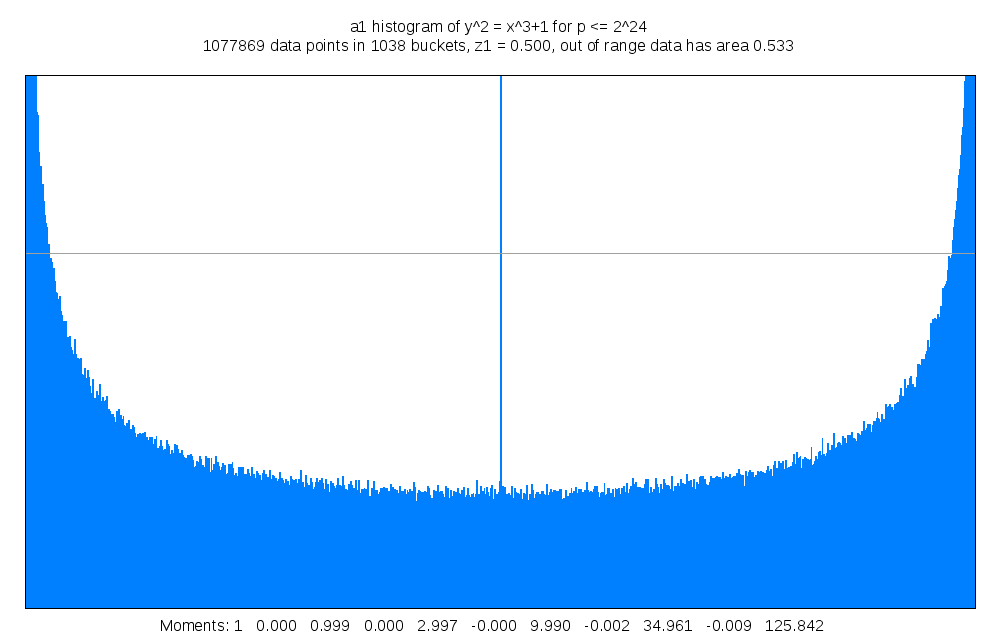
\includegraphics[scale=.3]{plots/Sato-Tate_CM.png}
\end{center}

The Sato-Tate conjecture is an analogous prediction for elliptic curves 
without complex multiplication. 

\begin{conjecture}[Sato-Tate]
Let $E$ be a non-CM elliptic curve over $\dQ$. Then the sequence 
$\{b_p(E)\}_p$ is equidistributed in $[-1,1]$ with respect to the 
measure 
\[
  \frac{2}{\pi} \sqrt{1-t^2}\, dt \text{.}
\]
\end{conjecture}

Here is the example $y^2=x^3+x+1$, also taken from Sutherland's web page. 

\begin{center}
  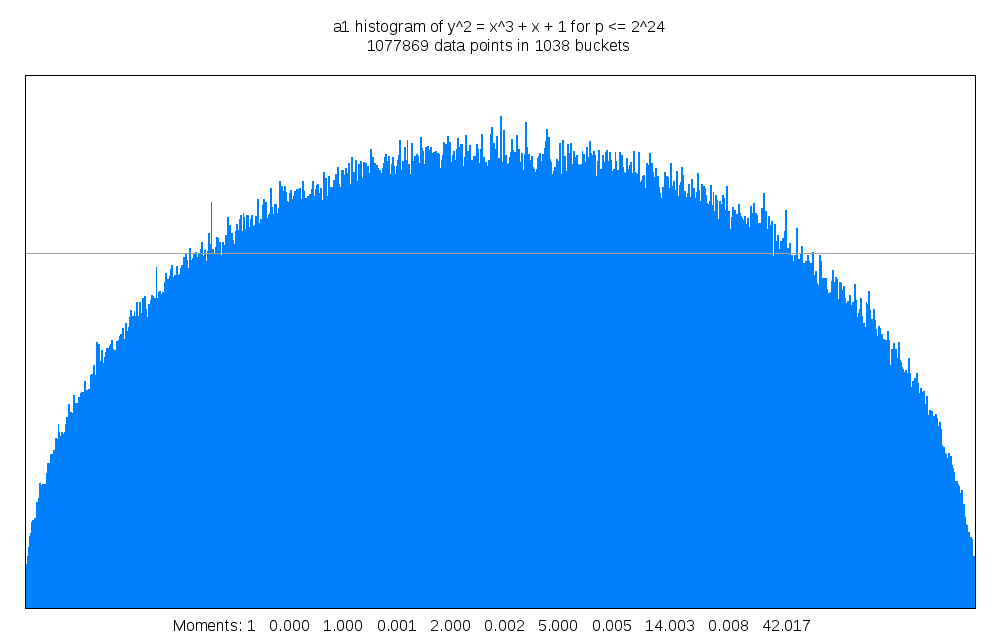
\includegraphics[scale=.3]{plots/Sato-Tate_nonCM.png}
\end{center}


\begin{theorem}[Barnet-Lamb, Geraghty, Harris, Taylor]
The Sato-Tate conjecture is true. 
\end{theorem}
\begin{proof}
See \cite[8.3]{bght09} for a (as yet unrefereed) proof. 
\end{proof}

There is a refined version of the Sato-Tate conjecture. Let 
$\rho=\{\rho_\ell:G_\dQ \to GL(2,\dZ_\ell)\}$ be a strictly compatible family 
of $\ell$-adic representations in the sense of \cite[ch.1]{se68}. For almost 
all primes $p$, the characteristic polynomial of $\rho_\ell(\arithfrob_p)$ will be 
of the form $t^2 - a_p t + p$. Assume $\rho$ is \emph{pure} in the sense that 
the roots $\alpha_p,\bar\alpha_p$ of $t^2-a_p t+p$ are $q$-Weil. 

\begin{conjecture}[Lang-Trotter]
For any integer $n$ and imaginary quadratic field $k$, there are constants 
$C(n,\rho)$ and $C(k,\rho)$ such that 
\begin{align*}
  \#\{ p\leqslant x : \dQ(\alpha_p) = k\} &\sim C(k,\rho) \frac{\sqrt x}{\log x} \\
  \#\{p\leqslant x : a_p = n\} &\sim C(n,\rho) \frac{\sqrt x}{\log x} \text{.}
\end{align*}
\end{conjecture}

See the introduction to \cite{lt76} for the original statement and some 
motivation. 





% on 11-21-2013
\subsection{Some computations}

Let $d=157$. We hope to show that $d$ is congruent, i.e. that is is the area 
of a right triangle with rational side lengths. In other words, the curve 
$C_d$ defined as the solution set to 
\begin{align*}
  a^2+b^2 &= c^2 \\
  a b/2 &= d
\end{align*}
has a rational point. We have seen that this is equivalent to the elliptic 
curve $E_d:y^2=x^3-d^2 x$ having positive rank. 

We'll use Sage to do this. Sage can be accessed online at 
\url{http://sagenb.com/}, or just type \texttt{sage} in the command line of a 
computer that has Sage installed. 

In Sage, the constructor 
$\mathtt{EllipticCurve([}a_1,a_2,a_3,a_4,a_6\mathtt{])}$ returns the 
elliptic curve 
\[
  y^2 + a_1 x y + a_3 y = x^3 + a_2 x^2 + a_4 x + a_6 \text{.}
\]
The simpler constructor 
$\mathtt{EllipticCurve([}a_4,a_6\mathtt{])}$ returns the elliptic curve 
$y^2 = x^3+a_4 x + a_6$. Sage will return an error if the curve you try to 
construct is singular. Since we are interested in the curve 
$E_{157}:y^2=x^3-157^2 x$, we define 
\begin{sageblock}
E = EllipticCurve([-157^2, 0])
\end{sageblock}
If we had wanted to define an elliptic curve over a finite field $\dF_q$, we 
would make sure some of the coefficients were elements of $\dF_q$, as in 
\texttt{EllipticCurve([GF(5)(1), 1])}. We can compute the conductor of 
by \texttt{E.conductor()}; in our case $E_{157}$ has conductor 
$\sage{factor(E.conductor())}$. Usually one can compute the rank 
\texttt{E.rank()} and generators for the Mordell-Weil group 
\texttt{E.gens()}. In our case, these return a warning. Sage's usual algorithm 
was not able to determine the rank of $E_{157}$, and it asks you to do a 
two-descent. We do this: 
\begin{sageblock}
E.two_descent(second_limit=13)
\end{sageblock}
\begin{sagesilent}
P = E.gens()[0]
x,y = P[0], P[1]
pair = (abs((157^2-x^2)/y), abs(2*157*x/y))
\end{sagesilent}
As Sage does the $2$-descent, it outputs a bunch of text describing what it 
does (essentially a computation of $E(\dQ)/2$ and 
$\sha(E)[2]$). Once the $2$-descent is complete, we can compute the rank to be 
$\sage{E.rank()}$ and a generator to be 
\[
  \sage{P} \text{.}
\]
This corresponds to a triangle with the shorter two sides being 
\[
  \sage{pair} \text{.}
\]

There are a number of other things that Sage can do with elliptic curves. To 
make computations faster, let's try the elliptic curve 
\begin{sageblock}
E = EllipticCurve([4,6])
\end{sageblock}
described by the equation $\sage{E}$. This curve has rank $\sage{E.rank()}$ and 
generator $\sage{E.gens()[0]}$. We can do computations with points on our 
curve: 
\begin{sageblock}
P = E.gens()[0]
5*P # as an element of E(Q)
P.height() # Neron-Tate height of P
\end{sageblock}
A lot of analytic data can be computed: 
\begin{sageblock}
E.torsion_subgroup() # trivial for this curve 
L = E.lseries().dokchitser() # the L-function of E
L(1) # looks like zero
L.derivative(1,2) # non-zero, so r_an<=1
E.root_number() # sign in function equation (=-1, so r_an is odd) 
E.regulator() 
E.sha().an() # predicted order assuming BSD
\end{sageblock}

A fantastic place to learn more about Sage is its documentation page at 
\url{http://www.sagemath.org/doc/}. 






\subsection{The Sato-Tate conjecture and Haar measures}

Let $E$ be an elliptic curve over $\dQ$. Recall we defined 
$b_p(E) = a_p(E)/2\sqrt p$. If $E$ has CM, then the $b_p$ are 
uniformly distributed in $[-1,1]$ with respect to the measure 
\[
  \frac 1 2 \delta_0 + \frac{dt}{2\pi\sqrt{1-t^2}} \text{,}
\]
and if $E$ is not CM, then the $b_p$ are uniformly distributed with respect to 
\[
  \frac{2}{\pi} \sqrt{1-t^2}\, dt \text{.}
\]
This has a natural reformulation which makes generalization easier. The 
characteristic polynomial of $\rho_{E,\ell}(\arithfrob_p)$ is 
$t^2-a_p t + p$. If we normalize to have roots with absolute value $1$, we get 
$\varphi_p = t^2 - \frac{a_p}{\sqrt p} t + 1$. This is the characteristic 
polynomial of a unique conjugacy class in $\operatorname{SU}(2)$. If we write 
$X$ for the space $\operatorname{SU}(2)^\natural$ of 
conjugacy classes in $\operatorname{SU}(2)$, then $p\mapsto \varphi_p$ can be 
thought of as a map $\{\text{primes}\} \to X$. Embed $\operatorname{U}(1)$ in 
$\operatorname{SU}(2)$ by the diagonal, and let $K=N(\operatorname{U}(1))$ be 
its normalizer. The group $K$ is compact, so it has a unique normalized Haar 
measure.

\begin{theorem}
If $E$ is an elliptic curve with complex multiplication, then the 
set $\{\varphi_p(E)\}\subset \operatorname{SU}(2)^\natural$ is 
equidistributed with respect to the pushforward of the normalized Haar measure 
on $N(\operatorname{U}(1))$. 
\end{theorem}
\begin{proof}
This is a restatement of \autoref{thm:deuring-hecke}. To see this, note 
that the trace map induces an isomorphism 
\[\xymatrix{
  \trace : \operatorname{SU}(2)^\natural \ar[r]^-\sim 
    & [-2,2] \text{.}
}\]
The group $K=N(\operatorname{U}(1))$ has two connected components, both 
isomorphic to $S^1$:
\[
  K = 
  \left\{\begin{pmatrix} 
    z & \\ 
    & \bar z 
  \end{pmatrix} : |z|=1 \right\} 
  \cup \left\{\begin{pmatrix}
         & -z\\ 
         \bar z & 
       \end{pmatrix} : |z|=1\right\} \text{.}
\]
The first connected component is mapped to $[-2,2]$ via 
$z\mapsto 2\Re (z)$, and the second is mapped via $z\mapsto 0$. It is easy to 
check that the pushforward of the Haar measure on $K$ is exactly 
$\frac 1 2 \delta_0 + \frac{dt}{2\pi \sqrt{4-t^2}}$. 
\end{proof}

For non-CM elliptic curves, let $K=\operatorname{SU}(2)$. Then the Sato-Tate 
conjecture states that $\{\varphi_p\}\subset \gl{2}{\dC}^\natural$ is 
uniformly distributed with respect to the pushforward of the normalized Haar 
measure on $K$. To see this, check that the pushforward by the trace of the 
normalized Haar measure on $K$ to $[-2,2]$ is $\frac{1}{2\pi} \sqrt{4-t^2} dt$. 

More generally, let $A$ be a $d$-dimensional abelian variety over $\dQ$, and 
let $\ell$ be a prime at which $A$ has good reduction. For any prime $p$ of 
good reduction, we have the characteristic polynomial $P_{A_p}$ of the 
Frobenius at $p$ acting on $T_\ell A$. The roots of this polynomial are 
$p$-Weil, so if we write $P_{A_p}(t) = \prod (t-\omega_i)$, then the polynomial 
$\varphi_p(A) = \prod \left(t-\frac{\omega_i}{\sqrt p}\right)$, has roots with 
absolute value $1$. Then by \cite[13.1]{ka88}, $\varphi_p(A)$ determines a 
conjugacy class in $\operatorname{SU}(2 d,\dC)$. As before, we think of 
$\varphi(A)$ as a map 
$\{\text{good primes}\}\to \operatorname{GL}(2 d,\dC)^\natural$. 

\begin{conjecture}[Serre]
There exists a compact real Lie group $K$ in $\gl{2d}{\dC}$ such 
that $\{\varphi_p(A)\}\subset \gl{2d}{\dC}^\natural$ is equidistributed with 
respect to the pushforward of the normalized Haar measure on $K$. 
\end{conjecture}

There is a conjectural prediction of the group $K$, which we will treat in the 
next section. 





\subsection{Motives and the refined Sato-Tate conjecture}

The following mostly follows Serre's original paper \cite{se94}, but see 
\cite{se12} for a more elementary and explicit approach. 

Let $k$ be a field, and let $X$ be an $n$-dimensional smooth variety over $k$. Write 
$\chow(X) = \chow^\bullet(X)$ for the Chow ring of $X$, consisting of algebraic 
cycles modulo rational equivalence. The intersection product makes $\chow(X)$ 
into a commutative unital ring -- for details, see \cite[8.3]{fu98}. There is a 
natural ``composition'' map 
\begin{equation*}\tag{$*$}\label{eq:compose-cycles}
  \chow(Y\times Z)\otimes \chow(X\times Y) \to \chow(X\times Z) \text{,}
\]
defined by 
$g\circ f = \pi_{X\times Z, \ast}(\pi_{Y\times Z}^\ast g\cdot \pi_{X\times Y}^\ast f)$. 
This satisfies all of the natural linearity and functoriality properties one 
would expect \cite[16.1]{fu98}. 

There is a canonical ``degree map'' $\deg:\chow^n \to \dZ$, and we say a cycle 
$\alpha \in \chow^r(X)$ is \emph{numerically equivalent to zero} if 
$\deg(\alpha\cdot \beta)=0$ for all $\beta\in \chow^{n-r}(X)$. Write 
$\chow_\text{num}(X)$ for the quotient of $\chow(X)$ by the (graded) ideal 
generated by 
\[
  \{\alpha\in \chow(X) : \alpha\text{ is numerically equivalent to zero}\} \text{.}
\]

\begin{definition}
Let $k$ be a field. A \emph{(pure) motive over $k$} is a triple 
$(X,e,r)$, where $X$ is a smooth projective variety over $k$, 
$e\in \chow_\textnormal{num}(X\times X)_\dQ$ is an idempotent, and 
$r\in \dZ$. 
\end{definition}

See \cite[4.1.3]{an04} for details. One defines a morphism 
$(X,e,r) \to (Y,f,s)$ to be an element of 
\[
  f\cdot \chow^{\dim X - r - s}(X\times Y)_\dQ\cdot e \text{.}
\]
Morphisms are composed via the ``composition map'' \eqref{eq:compose-cycles}. 

With this, write $\motives(k)$ for the category of (numerical) motives over 
$k$. Let $\mathsf{SmProj}_k$ be the category of smooth projective varieties 
over $k$, and let $h:\mathsf{SmProj}_k \to \motives(k)$ be the functor 
$X\mapsto (X,\Delta_X,0)$. The category $\motives(k)$ is obviously $\dQ$-linear, and 
has a Tannakian structure induced by $h(X)\otimes h(Y) = h(X\times Y)$. In 
fact, $\motives(k)$ is a semisimple abelian category \cite{ja92}. One should 
think of a Weil cohomology theory as a functor 
$\h:\motives(k) \to \mathsf{grAlg}_L$ for some field $L$ (c.f. 
\cite[4.2.5.1]{an04}). 

Write $1=\h(\dA^0)$ for the trivial motive. Since every variety has a unique 
morphism $X\to \dA^0$, there is a unique morphism $1\to M$ for every motive 
$M$. The rational point $\infty\in \dP^1$ determines a splitting of 
$1\to h(\dP^1)$, hence a direct sum decomposition $h(\dP^1)=1\oplus 1(-1)$, 
where $1(-1)$ is the motive $(\dP^1,[\infty]\times \dP^1,0)$. We define 
$1(r)=1(-1)^{\otimes(-r)}$; these are called \emph{Tate motives}. In general, 
put $M(r) = M\otimes 1(r)$. There is a decomposition 
$h(\dP^n) = 1\oplus \cdots \oplus 1(-n)$. If $A$ is a $d$-dimensional abelian 
variety over $k$, then there is a unique decomposition 
$h(A)=h^0(A)\oplus \cdots \oplus h^{2 d}(A)$ in $\motives(k)$ such that 
$[n]$ acts as multiplication by $n^i$ on each $h^i(A)$ \cite[13.29]{gm13}. %\cite[3.1]{ku94}. 
What is more, there are canonical isomorphisms 
$h^i(A)\simeq \bigwedge^i h^1(A)$, inducing an isomorphism 
$h(A)\simeq \bigwedge^\bullet h^1(A)$ (13.47, loc. cit.). 


Let $k$ be a number field, and choose an embedding 
$\sigma:k \hookrightarrow\dC$. We have a Betti realization functor 
$\h_\sigma:\motives(k) \to \mathsf{grAlg}_\dQ$, assigning to a motive 
$M = (X,e,r)$ the vector space 
\[
  \h_\sigma(M) = e^\ast \cdot \h_\text{sing}^\bullet(X(\dC), \dQ) \otimes \h^2_\text{sing}(\dP^1)^{\otimes (-r)}
\]
Assuming Grothendieck's standard conjectures, the functor $\h_\sigma$ is a 
\emph{fiber functor}, so $\mathsf{M}(k)$ is equivalent to the category of 
representations of the (pro-reductive) \emph{motivic Galois group} 
\[
  G_\text{mot}(k) = \aut^\otimes(\h_\sigma) = \left\{(x_M)\in \prod_{M\in\motives(k)} \operatorname{GL}(\h_\sigma M) : x_M\circ f^\ast = f^\ast\circ x_N\text{ for }f:M\to N \right\}\text{.}
\]
For a motive $M$, let $G_M$ be the automorphism group of the restriction of the 
fiber functor to the largest Tannakian subcategory of $\motives(k)$ containing 
$M$. There are obvious projections from $G_\text{mot}(k)$ to the groups $G_M$. 

Let $M$ be a motive. There is a map $w:\dG_m \to G_M$, induced by the grading 
$\h_\sigma M = \bigoplus \h_\sigma^d(M)$. The action of $a\in \dG_M$ on the 
$d$-th piece is by $a^{-d}$. For example, if $E$ is an elliptic curve without 
complex multiplication, then for $M=h^1(E)$, $G_M=\operatorname{GL}(2)$ and 
$w:\dG_m \to \operatorname{GL}(2)$ is the inverse of the canonical injection. 
(\textbf{this is not correct!})

For a motive $M$, there are $\ell$-adic realizations $\h_\ell(M)$ coming from 
\'etale cohomology. After we fix a prime $\ell$, the representation 
$\rho_{M,\ell}$ is unramified at all but finitely many places. For those 
unramified places $v$, put 
$\varphi_v(M) = w(N v^{1/2}) \rho_{M,\ell}(\arithfrob_v)$. 

Let $T=1(-1)$ be the Tate motive, and let $t:G_\text{mot}(k) \to G_T$ be the 
canonical projection. For any motive $M$, let $G_M^1$ be the image of 
$\ker(t)$ under the projection $G_\text{mot}(k) \to G_M$. 

\begin{conjecture}[Serre]
Let $M$ be a motive over a number field $k$. Let $K$ be a maximal compact 
subgroup of $G_M^1$. The elements $\varphi_v(M)$ have eigenvalues in 
$\bar\dQ$, and determine a unique conjugacy class (independent of $\ell$) 
$\varphi_v(M) \in G_M^1(\dC)^\natural$. The set 
$\{\varphi_v(M)\}\subset G_M^1(\dC)^\natural$ is equidistributed with respect 
to the pushforward of the normalized Haar measure on $K$. 
\end{conjecture}






\subsection{The Bloch-Kato conjecture}

Let $E$ be an elliptic curve over $\dQ$. Recall that the (strong) Birch and 
Swinnerton-Dyer conjecture is the formula 
\[
  \lim_{s \to 1} \frac{L(E,s)}{(s-1)^{\rank E}} = \frac{\Omega_E \regulator_E \# \sha(E) \prod_p c_p}{\# E(\dQ)_\text{tors}^2} \text{,}
\]
together with the claim that everything involved is well-defined and finite. 
For a number field $k$, recall that the \emph{Dedekind zeta function} of $k$ 
is the series 
\[
  \zeta_k(s) = \sum_{\fa\subset \fo_k} \frac{1}{(N\fa)^s} \text{,}
\]
where $N\fa = [\fo_k:\fa]$ for an ideal $\fa$. It is a theorem that $\zeta_k$ 
has an analytic continuation to $\dC\smallsetminus 1$. The pole at $s=1$, and 
we have the following analytic \emph{class number formula}. Let $r$ be the 
order of the pole of $\zeta_k$ at $1$, and let $r_1,r_2$ be the number of 
real (resp. complex) places of $k$. Let $h_k$ be the class number of $k$, $d_k$ 
be the discriminant of $k$. Then 
\[
  \lim_{s \to 1} \frac{\zeta_k(s)}{(s-1)^r} = \frac{2^{r_1} (2\pi)^{r_2}|d_k|^{-1/2} \regulator_k h_k}{\# \mu(k)} \text{.}
\]

The Birch and Swinnerton-Dyer conjecture as well as the class number formula 
are both special cases of a very far-reaching generalization called the 
\emph{Bloch-Kato conjecture}. 

\textbf{(add BSD for abelian varieties, brief statement of Bloch-Kato)}

Follow \cite[III]{la91} for definition of regulator of abelian variety, 
general BSD. 






% !TEX root = 7390-notes.tex





\section{Some theorems of Faltings}





\subsection{Background and Tate's conjecture}

The goal of this section is to describe the relationships between a web of 
conjectures that Faltings proved in his groundbreaking paper 
\cite{fa86}. 

Let $A$ be a $d$-dimensional abelian variety over a field $k$. As usual, we 
write $\bar k$ for the algebraic closure of $k$ and $G_k=\gal(\bar k/k)$ for 
the absolute Galois group of $k$. Fix a prime $\ell$ invertible in $k$. The 
groups $A[\ell^n] = \{x\in A(\bar k):\ell^n x=0\}$ are abstractly isomorphic 
to $(\dZ/\ell^n)^{\oplus 2d}$, and carry a continuous action of $G_k$. They 
fit into an inverse system 
\[\xymatrix{
  A[\ell] 
    & A[\ell^2] \ar[l]_-\ell 
    & A[\ell^3] \ar[l]_-\ell 
    & \cdots \ar[l]
}\]
Put 
\[
  T_\ell A = \varprojlim A[\ell^n] = \left\{(x_n)\in \prod A[\ell^n] : \ell x_{n+1} = x_n\right\} \text{.}
\]
This is the \emph{$\ell$-adic Tate module of $A$}. As a $\dZ_\ell$-module, 
$T_\ell A \simeq \dZ_\ell^{\oplus 2 d}$. What makes $T_\ell A$ interesting is 
that it carries a continuous action of $G_k$, induced by the action of $G_k$ 
on the $A[\ell^n]$. In other words, after choosing a basis of $T_\ell A$, we 
have a continuous representation 
\[
  \rho_{A,\ell} : G_k \to \gl{2 d}{\dZ_\ell} \text{.}
\]

The action of $G_k$ on $T_\ell A$ factors through 
the smaller group $\operatorname{GSp}(2 n,\dZ_\ell)$ of symplectic simlitudes. 
One sees this via the \emph{Weil pairing}. There is, for any $n$ invertible in 
$k$, a natural perfect pairing $A[n]\times A^\vee[n] \to \mu_n$, defined at the 
level of schemes. For a prime $\ell$ invertible in $k$, these pairings patch 
together to give a perfect $G_k$-equivariant pairing 
$T_\ell A \times T_\ell A^\vee \to \dZ_\ell(1)$. After a choice of polarization 
$\lambda:A\to A^\vee$, we get an (alternating) pairing 
$T_\ell A\times T_\ell A\to \dZ_\ell(1)$. If $\ell$ is relatively prime to the 
degree of $\lambda$, then this pairing is perfect. In what follows, we will 
always assume this to be the case. For a proof of these facts in a pretty 
general setting, see \cite[11]{gm13}. 

It is natural to ask how much $\rho_{A,\ell}$ ``knows about'' $A$, especially 
if $k$ is a number field, or more generally, a finitely generated field. 

Let $X$ be a nice variety over a finitely generated field $k$. For each $i$, 
there is a canonical homomorphism 
\[
  \operatorname{cl}:\chow^i(X) \to \h^{2 i}(X_{k^s},\dQ_\ell)(i)\text{,}
\]
defined in \cite[VI 2.2.10]{de77}. One calls $\operatorname{cl}(Z)$ the 
cohomology class associated with a cycle $Z$. 

\begin{conjecture}[Tate]
The cycle map induces an isomorphism 
$\chow^i(X)\otimes\dZ_\ell \isomorphism \h^{2 i}(X_{k^s},\dQ_\ell)(i)^{G_k}$. 
\end{conjecture}

This is essentially Conjecture 1 in \cite{ta65}. Often, ``the Tate conjecture'' 
means the following special case. 

\begin{conjecture}[Tate]
Let $A,B$ be abelian varieties over a finitely generated field $k$. For any 
prime $\ell$ invertible in $k$, the natural map 
\[
  \hom_k(A,B)\otimes\dQ_\ell \to \hom_{G_k}(V_\ell A, V_\ell B) 
\]
is a bijection. 
\end{conjecture}

See the remarks after Conjecture 1 in Tate's paper, or 
\cite[IV.1.4]{fa84}, for a proof that the second version of the conjecture 
follows from the first. Another way of stating the (second version 
of the) Tate conjecture is that for any finitely generated field $k$, the 
functor $V_\ell:\mathsf{AbVar}_k^\text{iso} \to \mathsf{Rep}_{G_k}(\dQ_\ell)$ 
is fully faithful. 

\begin{example}
Let $k=\dF_q$ be a finite field. Then $G_k$ is naturally isomorphic to 
$\widehat\dZ$, the profinite completion of $\dZ$. Here $1\in \widehat\dZ$ 
corresponds to the \emph{arithmetic Frobenius} $\arithfrob_q\in G_{\dF_q}$, given by 
$x\mapsto x^q$. Representations 
$\rho:G_{\dF_q} \to \gl{n}{\dQ_\ell}$ are determined by 
$\rho(\arithfrob_q)$. If such a representation is semisimple, the 
\emph{Brauer-Nesbitt theorem} tells us that $\rho$ is determined by the 
characteristic polynomial of $\rho(\arithfrob_q)$. For an abelian variety $A$ over 
$\dF_q$, we know that the characteristic polynomial of 
$\rho_{A,\ell}(\arithfrob_q)$ is $P_A(t)\in \dZ[t]$, which determines $A$ up to 
isogeny by Honda-Tate theory. 
\end{example}

Since we will be using characteristic polynomials quite a lot, let us state a 
suitably general version of the Brauer-Nesbitt theorem. Fix a field $k$, and 
for an arbitrary group $G$, let $K_0(G)$ denote the Grothendieck group of 
finite-dimensional $k$-representations of $G$. By the ``characteristic 
polynomial'' of a representation $\rho:G \to \operatorname{GL}_k(V)$, we mean 
the map $\chi_\rho:G\to \Lambda(k)=1+t k\llbracket t\rrbracket$ defined by 
\[
  \chi_\rho(g) = \frac{1}{\det(1-\rho(g)\cdot t, V)} \text{.}
\]
Alternatively, $t\frac{d}{dt} \log \chi_\rho(g) = \sum \trace(\rho(g)^n)$. 

\begin{theorem}[Brauer-Nesbitt]
If $S$ spans $k[G]$ as a $k$-vector space, then the map 
$\chi:K_0(G) \to \Lambda(k)^S$ given by $[\rho]\mapsto \chi_\rho$ is an 
injection. 
\end{theorem}
\begin{proof}
This is Theorem 5.21 of \cite{eg11}. 
\end{proof}

\begin{corollary}
If $k$ has characteristic zero and 
$\rho_1,\rho_2:G \to \operatorname{GL}_k(V)$ are two semisimple representations 
with identical characters, then $\rho_1\simeq \rho_2$. 
\end{corollary}






% notes on 11-26-2013

\begin{theorem}[Faltings' isogeny theorem]
Let $A$ and $B$ be abelian varieties over a number field $k$. For any prime 
$\ell$, we have $\rho_{A,\ell}\simeq \rho_{B,\ell}$ as $G_k$-modules if and 
only if $A$ and $B$ are isogenous over $k$. 
\end{theorem}

From this, we see that we can fruitfully study $A$ via $\rho_{A,\ell}$. For 
example, the rank of an abelian variety only depends on its isogeny class, so 
$\rank A$ only depends on $\rho_{A,\ell}$. 

If $k$ is either finite or a global field, the representation $\rho_{A,\ell}$ 
is semisimple, so $\rho_{A,\ell}$ is determined by the characteristic 
polynomial of $\rho_{A,\ell}(\arithfrob_q)$. For this, one needs the 
\emph{\v Cebotarev density theorem}. 





\subsection{Image of Frobenius for number fields}

Fix a number field $k$, and a finite place $v$ of $k$. Let 
$\fp\subset \fo=\fo_k$ be the corresponding maximal ideal. Let $k_v$ be the 
completion of $k$ at $v$. We choose $\bar k\subset \overline{k_v}$; this gives 
a map $G_{k_v} \to G_k$, defined by $\sigma\mapsto \sigma|_{\bar k}$. This map 
is only well-defined up to conjugation. By Krasner's lemma, the map is an 
injection. Reduction modulo $\fp$ gives a homomorphism 
$G_{k_v} \to G_{\kappa_v}=\widehat\dZ$, where $\kappa_v = \fo_v/\fp$ is the 
residue field of $\fp$. This map is surjective, so we have an exact sequence 
(where we write $D_v$ for the image of $G_{k_v}$ in $G_k$):
\[\xymatrix{
  1 \ar[r] 
    & I_v \ar[r] 
    & D_v \ar[r] 
    & \widehat\dZ \ar[r] 
    & 1 \text{.}
}\]
The group $G_{\kappa_v}$ is procyclic, with generator 
$\arithfrob_{N v}$, where as usual $N v = \# \kappa_v$. Write $\arithfrob_v$ for a lift 
of $\arithfrob_{N v}$ to $D_v$. The element $\arithfrob_v\in G_k$ is only well-defined up 
to conjugacy and multiplication by $I_v$. 

As before, let $A$ be an abelian variety over $k$ with good reduction at $v$. 
Then (by definition) there exists an abelian scheme $\cA$ over $\fo_v$ whose 
generic fiber is $A_{k_v}$. The scheme $\cA$ fits into a commutative diagram 
with cartesian squares: 
\[\xymatrix{
  A_v \ar[r] \ar[d] 
    & \cA \ar[d] 
    & A_{k_v} \ar[l] \ar[d] \\
  \spec(\kappa_v) \ar[r] 
    & \spec(\fo_v) 
    & \spec(k_v) \ar[l] 
}\]
We have define $A_v=\cA_{\kappa_v}$. The property of being abelian is stable 
under base change, so $A_v$ is an abelian variety over $\kappa_v$, and we have 
a reduction map 
\[
  A(k_v) = \cA(\fo_v) \to \cA(\kappa_v) = A_v(\kappa_v) \text{.}
\]
Extending to algebraic closures, we get a map 
$A(\overline{k_v}) \to A_v(\overline{\kappa_v})$. This is a homomorphism with 
pro-$p$ kernel. Let $\ell\nmid v$ (i.e. $\ell$ is relatively prime to the 
residue characteristic of $v$). At the level of torsion, we have isomorphisms 
\[
  A(\overline{k_v})[\ell^n] \to A_v(\overline{\kappa_v})[\ell^n] \text{.}
\]
The map is injective because its kernel is pro-$p$, and it is surjective by 
cardinality considerations -- both groups have cardinality $(\ell^n)^{2 d}$). 
This gives us an isomorphism 
$A(\bar k)[\ell^n] = A(\overline{k_v})[\ell^n]\isomorphism A_v(\kappa_v)[\ell^n]$. 
These groups have (compatible) actions of $G_k$, $G_{k_v}$ and $G_{\kappa_v}$. In 
particular, the inertia group $I_v$ acts trivially on $A(\bar k)[\ell^n]$. 

It follows that $\arithfrob_v$, \emph{a priori} only well-defined up to conjugacy 
and multiplication by $I_v$, has a well-defined action on $A[\ell^n]$, and 
hence on $T_\ell A$. That is, we have the following theorem. 

\begin{theorem}\label{thm:ab-var-good}
Let $A$ be an abelian variety over $k$ with good reduction at $v$. Then for 
$v\nmid \ell$, we have  
\begin{enumerate}
  \item $\rho_{A,\ell}$ is unramified at $v$ (i.e. $\rho_{A,\ell}(I_v) = 1$) 
  \item $\rho_{A,\ell}(\arithfrob_v)$ is well-defined up to conjugacy and has 
    characteristic polynomial $P_{A_v}(t)$ with integer coefficients that do 
    not depend on $\ell$. 
\end{enumerate}
\end{theorem}
\begin{proof}
See \ref{sec:char-frob} for a definition of $P_{A_v}(t)$. This is Theorem 1, 
paired with the corollary to Theorem 3 in \cite{st68}. 
\end{proof}

Recall the \v Cebotarev density theorem. Let $k$ be a number field, $K/k$ a 
finite Galois extension. For $v$ unramified in $K/k$, there is a well-defined 
conjugacy class $\arithfrob_v\in \gal(K/k)^\natural$. \v Cebotarev's density theorem 
is essentially the Sato-Tate conjecture for the motive 
$h(\spec K)$, i.e. it predicts equidistribution of Frobenii, in the appropriate 
sense. 

\begin{theorem}[\v Cebotarev]
Let $K/k$ be a finite Galois extension of number fields with Galois group $G$. Then 
$\{\arithfrob_v\}\subset G^\natural$ is equidistributed with respect to the Haar 
measure on $G$. 
\end{theorem}
\begin{proof}
See \cite[1.2.2]{se68} for a beautiful proof using the representation theory of 
compact groups. 
\end{proof}

Recall that the statement ``$\{\arithfrob_v\}\subset G^\natural$ is 
equidistributed'' means that for any conjugacy class $C\subset G$, we have 
\[
  \lim_{x \to \infty} \frac{\{\# v : N v \leqslant x \text{ and } \arithfrob_v\in C\}}{\# \{v:N v\leqslant x\}} = \frac{\# C}{\# G}
\]
It follows that each conjugacy class in $G$ is Frobenius for infinitely many 
primes.  

For example, if $k=\dQ$ and $K=\dQ(\zeta_n)$, then $\gal(K/\dQ)$ is naturally 
isomorphic to $(\dZ/n)^\times$. For $p\nmid n$, the Frobenius $\arithfrob_p$ 
corresponds to $p\in (\dZ/n)^\times$. Dirichlet's theorem says that for 
$a\in (\dZ/n)^\times$, there exist infinitely many $p$ such that 
$p\equiv a\pmod n$, i.e. the \v Cebotarev density theorem holds for cyclotomic 
extensions. 

\begin{theorem}[N\'eron-Ogg-Shafarevich]
Let $A$ be an abelian variety over a number field $k$. Let $v$ be a place of 
$k$, and let $\ell$ be a prime with $v\nmid \ell$. Then $A$ has good reduction 
at $v$ if and only if $\rho_{A,\ell}$ is unramified at $v$. 
\end{theorem}
\begin{proof}
This is the main theorem of \cite{st68}. 
\end{proof}





\subsection{\texorpdfstring{$L$}{L}-function of an abelian variety}

Let's define the $L$-function of an arbitrary abelian variety over a number 
field $k$. For a place $v$ of $k$, choose a prime $\ell$ with $v\nmid \ell$. 
The action of $\arithfrob_v$ on $T_\ell A$ is only well-defined up to the action of 
$I_v$, but $(T_\ell A)_{I_v} = T_\ell A / \{\sigma x-x:x\in I_v\}$ has a 
well-defined action of $\arithfrob_v$. Define
\begin{align*}
  L_v(A,t) &= \det\left(1-\rho_{A,\ell}(\arithfrob_v)\cdot t,(T_\ell A)_{I_v}\right) \\
  L(A,s) &= \prod_{v\nmid \infty} L_v\left(A,(N v)^{-s}\right)^{-1} \text{.}
\end{align*}
This is well-defined by the following theorem. 

\begin{theorem}
Let $A$ be an abelian variety over a number field $k$. For any finite place 
$v$, the local factor $L_v(A,t)$ is an element of $\dZ[t]$ that does not depend 
on $\ell$. 
\end{theorem}
\begin{proof}
For $v$ a place of good reduction, this is \autoref{thm:ab-var-good}. The 
general case is a bit more subtle. First, note that 
\[
  \det(1-\rho_{A,\ell}(\arithfrob_v)\cdot t,(T_\ell A)_{I_v}) 
    = \det(1-\rho_{A,\ell}(\arithfrob_v^{-1}),((T_\ell A)^\vee)^{I_v}) \text{.}
\]
The Weil pairing gives us an isomorphism $(T_\ell A)^\vee= T_\ell A(-1)$, 
and because the $\ell$-adic cyclotomic character is unramified at 
$v\nmid \ell$, we get $((T_\ell A)^\vee)^{I_v} = (T_\ell A)^{I_v}(-1)$. 

Let $\cA$ be the N\'eron model for $A$ over 
$\fo_v$, and let $A_v$ be the connected component of the identity in 
$\cA_{\kappa_v}$. By Lemma 2 of \cite{st68}, there is a $D_v$-equivariant 
isomorphism $(T_\ell A)^{I_v} \to T_\ell A_v$. 

Chevalley's theorem (see \cite{co02} for a modern proof) gives us a linear 
algebraic group $G\subset A_v$ such that $B=A_v/G$ is an abelian variety. In 
other words, we have a short exact sequence 
\[\xymatrix{
  1 \ar[r] 
    & G \ar[r] 
    & A_v \ar[r] 
    & B \ar[r] 
    & 0 \text{.} 
}\]
The group $G$ splits into a product $G=T\times U$, where $T$ is a (possibly 
non-split) torus and $U$ is unipotent. The group $U$ will be an iterated 
extension of copies of $\dG_a$, so $T_\ell U=0$. 

Let $\widehat T=\hom_{\bar k}(T_{\bar k},\dG_{m,\bar k})$ be the group of 
characters of $T$. This has an obvious continuous $G_k$-action, and there is a 
$G_k$-equivariant pairing 
\[
  T_\ell T \otimes \widehat T \to \dZ_\ell(1) \text{,}
\]
given by $(x_n)_n\otimes \chi \mapsto (\chi(x_n))_n$. It is easy to see (by 
base-change to $\bar k$) that this pairing is nondegenerate, so we have a 
$G_k$-isomorphism $T_\ell T \simeq \widehat T^\vee \otimes \dZ_\ell(1)$. 
We obtain 
\[
  \det(1-\rho_{A_v,\ell}(\arithfrob_v)\cdot t) = \det(1-\rho_{B,\ell}(\arithfrob_v)\cdot t,T_\ell B) \cdot \det(1-\arithfrob_v^{-1}\cdot t,\widehat T\otimes \dZ_\ell) \text{.}
\]
Since $B$ does not depend on $\ell$ and $G_k$ acts on 
$\widehat T\otimes \dZ_\ell$ via its action on $\widehat T$, the characteristic 
polynomial of Frobenius is an element of $\dZ[t]$ independent of $\ell$. 
\end{proof}

Let's check that our definition of $L(A,s)$ agrees with our previous definition 
in the case that $A=E$ is an elliptic curve over $k$. If $E$ has good reduction 
at $v$, $(T_\ell E)_{I_v}=T_\ell E$ and there is nothing to prove. If $E$ has 
bad reduction at $v$, then as before let $E_v$ be the connected component 
of the special fiber of the N\'eron model at $v$. Recall that $E$ has 
\emph{multiplicative reduction} at $v$ if $E_v$ is a torus, and \emph{additive 
reduction} if $E_v$ is unipotent. Clearly  
\[
  \rank_{\dZ_\ell} (T_\ell E)^{I_p}
  =
  \begin{cases}
    2 & \text{good reduction} \\
    1 & \text{mult. reduction} \\
    0 & \text{add. reduction}
  \end{cases}
\]
If $E$ has split multiplicative reduction at $v$, then the local factor 
$L_v(E,t)$ is the (reverse of) the characteristic polynomial of Frobenius 
acting on $T_\ell \dG_m(-1) = \dZ_\ell$. On the other hand, if $E$ has 
nonsplit multiplicative reduction at $v$, then by \cite[III,2.5]{si06}, 
$E_v$ splits after a quadratic base-change, from which we see that 
$\arithfrob_v$ acts on $\widehat E_v$ as $-1$, whence the following: 
\[
  L_v(E,t) = 
    \begin{cases}
      1 & \text{additive reduction} \\
      1-t & \text{split multiplicative reduction} \\
      1+t & \text{nonsplit multiplicative reduction} \\
      1 - a_p t + p t^2 & \text{good reduction} 
    \end{cases}
\]

The function $L(A,s)$ should have an analytic continuation, functional equation, 
it should satisfy BSD ($\ord_{s=1} L(A,s) = \rank_\dZ A(\dQ)$), and a ``fancy BSD'' 
with a precise prediction of the coefficient in Taylor series. 
By the Weil conjectures, the function $L(A,s)$ converges on some region 
$\{\Im s>c\}$. 





\subsection{Tate conjectures and isogenies}

Much of the rest of this section follows Lang's excellent survey 
\cite{la91} and the more technical \cite{fa84}. We begin with a useful fact. 

\begin{theorem}\label{thm:trace-determines-rep}
Let $k$ be a number field and $\rho_1,\rho_2:G_k \to \gl{n}{\dZ_\ell}$ 
continuous semisimple representations. If 
$\trace \rho_1(\arithfrob_v) = \trace \rho_2(\arithfrob_v)$ for all $v$ in a density-one 
set of places, then $\rho_1\simeq \rho_2$. 
\end{theorem}
\begin{proof}
By the \v Cebotarev density theorem, the set $\{\arithfrob_v\}\subset G_k^\natural$ 
is dense. It follows that $\trace \rho_1 = \trace \rho_2$, so the conclusion 
follows from the Brauer-Nesbitt theorem. 
\end{proof}

We are mainly interested in the case when $\rho_1=\rho_{A,\ell}$ and 
$\rho_2=\rho_{B,\ell}$ for $A,B$ abelian varieties over $k$. The theorem tells 
us that if $P_{A_v} = P_{B_v}$ for almost all primes, then 
$\rho_{A,\ell}\simeq \rho_{B,\ell}$. A morphism $f:A\to B$ of abelian varieties 
induces a $G_k$-equivariant morphism $f_\ast:T_\ell A \to T_\ell B$. If $f$ is 
an isogeny, then $f_\ast$ is an isomorphism after tensoring with $\dQ$. In 
particular, if we think of $\rho_{A,\ell}$ as a $\dQ_\ell$-representation, then 
$\rho_{A,\ell}\simeq \rho_{B,\ell}$. It follows that $A$ and $B$ have the same 
bad primes. 

The following theorem was conjectured by Tate, and proved when $k$ is a finite 
field. 

\begin{theorem}[Faltings]
Let $k$ be a finitely generated field and $A,B$ abelian varieties over $k$. 
Then 
\begin{enumerate} % TODO: $\rho_{A,\ell}$ is only semisimple after tensoring with Q!
  \item (Semisimplicity) $V_\ell A$ is a semisimple $G_k$-module. 
  \item (Tate conjecture) The natural map
    \[
      \hom(A,B)\otimes\dZ_\ell \to \hom_{G_k}(T_\ell A,T_\ell B)
    \]
    is an isomorphism. 
\end{enumerate}
\end{theorem}
\begin{proof}
See \cite{fa84} for a proof when $k$ has characteristic zero. Alternatively, 
see \cite[IV.2.5]{mi-av} for a proof that semisimplicity and the Tate 
conjecture follow from \autoref{thm:finiteness-I}. 
\end{proof}

\begin{corollary}[Isogeny theorem]\label{thm:isogeny-thm}
Abelian varieties $A$ and $B$ over a number field $k$ are isogenous if and only 
if $\rho_{A,\ell}$ and $\rho_{B,\ell}$ are isomorphic. 
\end{corollary}
\begin{proof}
We've already seen that if $A$ and $B$ are isogenous, then 
$\rho_{A,\ell}\simeq \rho_{B,\ell}$. The Tate conjecture gives us an 
isomorphism 
\[\xymatrix{
  \hom(A,B)\otimes\dZ_\ell \ar[r]^-\sim 
    & \hom_{G_k}(T_\ell A,T_\ell B) \text{.}
}\]
Assuming $\rho_{A,\ell}$ and $\rho_{B,\ell}$ are isomorphic, we can choose 
a specific isomorphism $f:\rho_{A,\ell}\to \rho_{B,\ell}$. Since 
$\hom_{G_k}(T_\ell A,T_\ell B)$ is a finite rank $\dZ_\ell$-module isomorphic 
to $\hom(A,B)\otimes \dZ_\ell$, the space $\hom(A,B)$ is dense in 
$\hom_{G_k}(T_\ell A,T_\ell B)$. The property ``$f:T_\ell A\to T_\ell B$ is an 
isomorphism'' is open, so there exists $\varphi:A\to B$ such that 
$\varphi_\ast$ is an isomorphism. We claim that $\varphi$ is an isogeny. 
Indeed, let $C=(\ker\varphi)^\circ\subset A$. If $C\ne 0$, then 
$\rank T_\ell C > 0$. This cannot be, because $\varphi_\ast(T_\ell C) = 0$ and 
$\varphi_\ast$ is an isomorphism. Thus $C=0$, so $\ker \varphi$ is finite. By 
dimension considerations, $\varphi$ is an isogeny. 
\end{proof}
By \cite[V.3.2]{fa84}, if $\rho_{A,\ell}\simeq \rho_{B,\ell}$, there actually 
exists an isogeny $f:A\to B$ with $\ell\nmid \deg f$. 

Choose a finite place $v$ of $k$ at which $A$ has good reduction. The 
polynomial $P_{A_v}(t)$ is integral, monic, and has degree $2 d$. So we can 
write 
\[
  P_{A_v}(t) = t^{2 d} - a_v(A) t^{2 d-1} + \cdots 
\]
where $a_v(A)=\trace\rho_{A,\ell}(\arithfrob_v)\in \dZ$. We have 
$|a_v(A)|\leqslant 2 g \sqrt{N v}$, since the roots of $P_{A_v}$ have 
absolute value $\sqrt{N v}$. 

If $A=E$ is an elliptic curve over $\dQ$, then this definition of $a_v(E)$ 
agrees with the the standard definition $a_p(E)=p+1-\# E(\dF_p)$. If 
$C$ is a nice curve over $\dQ$ of genus $g$, then for 
$J=\jac C$, we have $\# C(\dF_p) = p+1-a_p(J)$. 

\begin{theorem}
Let $A$ and $B$ be abelian varieties over a number field $k$. Let $S$ be a 
density-zero set of places of $k$, containing the infinite places, as well as 
the bad places for $A$ and $B$. Then $A$ is isogenous to $B$ if and only if 
$a_v(A)=a_v(B)$ for all $v\notin S$. 
\end{theorem}
\begin{proof}
Fix a prime $\ell$. If $A$ and $B$ are isogenous, then 
$\rho_{A,\ell}\simeq \rho_{B,\ell}$, so 
$a_v(A)=\trace(\rho_{A,\ell}(\arithfrob_v))=\trace(\rho_{B,\ell}(\arithfrob_v))=a_v(B)$ 
for all places $v\notin S\cup\{\ell\}$. The converse is an immediate corollary 
of \autoref{thm:trace-determines-rep}. and the isogeny theorem 
(\autoref{thm:isogeny-thm}). 
\end{proof}

This theorem is not especially useful, because it requires checking 
$a_v(A)=a_v(B)$ at an infinite set of places. The following lemma and its 
corollary give us a way of capturing the isogeny class of an abelian variety 
using a finite amount of data. 





\subsection{Finiteness theorems}

\begin{lemma}[Faltings]
Let $k$ be a number field, $S$ a finite set of places, and $n\geqslant 1$ an 
integer. Then there is a finite set $T$ of places, disjoint from $S$ and 
depending only on $(k,S,n)$, such that if 
$\rho_1,\rho_2:G_{k,S} \to \gl{n}{\dZ_\ell}$ are continuous representations 
with $\trace\rho_1(\arithfrob_v) = \trace \rho_2(\arithfrob_v)$ for all $v\in T$, then 
$\rho_1\simeq \rho_2$. 
\end{lemma}
\begin{proof}
Without loss of generality, we can assume $S$ contains all places dividing 
$\ell$. Let $d = \ell^{2 n^2} = \# M_n(\dF_\ell)\times M_n(\dF_\ell)$. By 
Hermite's theorem, there are only finitely many extensions of $k$ unramified 
outside $S$ with degree $\leqslant d$. Let $K/k$ be a Galois extension 
containing all these and let $G=\gal(K/k)$. The \v Cebotarev density theorem 
tells us that there is a finite set $T$ (disjoint from $S$) of places of $k$ 
such that $G^\natural = \{\arithfrob_v:v\in T\}$. 

Now let $\rho_1,\rho_2$ be as in the statement of the lemma. Set 
$\rho=\rho_1\times\rho_2:G_{k,S} \to \gl{n}{\dZ_\ell}\times \gl{n}{\dZ_\ell}$. 
Let $R$ be the $\dZ_\ell$-subalgebra of 
$M_n(\dZ_\ell)\times M_n(\dZ_\ell)$ generated by the image of $\rho$. Note that 
$R$ is a free $\dZ_\ell$-module of rank at most $2 n^2$. We can consider the 
reduction of $\rho$ modulo $\ell$, i.e. $\bar\rho:G_k \to (R/\ell)^\times$. We 
know that $\# (R/\ell)^\times \leqslant d$, so $\bar\rho$ factors through $G$ 
as in the commutative diagram: 
\[\xymatrix{
  G_k \ar[r]^-{\bar\rho} \ar@{->>}[d] 
    & (R/\ell)^\times \\
  G \ar[ur]
}\]
It follows that $R/\ell$ is generated (as a group) by the images of 
$\{\rho([\arithfrob_v]):\in T\}$. By Nakayama's lemma, $R$ is generated as a 
$\dZ_\ell$-module by $\{\rho([\arithfrob_v]):v\in T\}$. 

Let $\varphi:R \to \dZ/\ell$ be the map $(g,h)\mapsto \trace g-\trace h$. This 
is a homomorphism of $\dZ_\ell$-modules. Assume $a_v(A)=a_v(B)$ for all 
$v\in T$. Then for $v\in T$, we have 
\[
  \varphi(\rho(\arithfrob_v)) = \trace \rho_{A,\ell}(\arithfrob_v) - \trace\rho_{B,\ell}(\arithfrob_v) = a_v(A)-a_v(B) = 0 
\]
This implies $\varphi=0$ since $\varphi$ vanishes on a set of generators of 
$R$. It follows that $\trace \rho_{A,\ell} = \trace\rho_{B,\ell}$. Since 
$\rho_{A,\ell}$ and $\rho_{B,\ell}$ are semisimple, this implies 
$\rho_{A,\ell}\simeq \rho_{B,\ell}$, and the isogeny theorem tells us that 
$A$ and $B$ are isogenous. 
\end{proof}

\begin{corollary}\label{lem:ab-var-fin-data}
Let $k$ be a number field, $S$ a finite set of places of $k$ and 
$d\geqslant 1$ an integer. Then there is a finite set $T$ of places of $k$, 
disjoint from $S$ and depending only on $(k,S,d)$, such that if $A$ and $B$ 
are $d$-dimensional abelian varieties with good reduction outside $S$, then 
$A$ and $B$ are isogenous if and only if $a_v(A)=a_v(B)$ for all $v\in T$. 
\end{corollary}

In the next section, we will prove the Mordell conjecture for number fields 
using Faltings proof of a finiteness result for abelian varieties. 

\begin{conjecture}[Shafarevich, for abelian varieties]
Fix a number field $k$ and a finite set $S$ of places, and an integer 
$d\geqslant 1$. Then there are only finitely many isomorphism classes of 
$d$-dimensional abelian varieties over $k$ with good reduction outside $S$. 
\end{conjecture}

Since isogenous abelian varieties have the same dimension and bad primes, 
the conjecture breaks up into two pieces. 

\begin{theorem}[Finiteness I]\label{thm:finiteness-I}
Let $A$ be an abelian variety over a number field $k$. Then there are only 
finitely many isomorphism classes of abelian varieties over $k$ which are 
isogenous to $A$. 
\end{theorem}
\begin{proof}
This is a \emph{very} brief sketch of the proof in \cite[V.3]{fa84}, which 
has several parts. First, one reduces to the case of principally polarized 
abelian varieties with semistable reduction everywhere. 

Next, one constructs the \emph{Faltings height} $h(A)$ of an arbitrary 
$d$-dimensional abelian variety $A$ over $k$ as follows. 
Let $\cA$ be the N\'eron model $\cA$ of $A$ over $\fo=\fo_k$, let 
$s:\spec(\fo) \to \cA$ be the identity section, and define 
\[
  \omega_{\cA/\fo} = \left(s^\ast \Omega_{\cA/\fo}^d\right)^\vee \text{.}
\]
This is a projective $\fo$-module of rank one. If $v$ is an infinite place of 
$k$ corresponding to $\sigma:k\hookrightarrow \dC$, the vector space 
$\omega_{\cA/\fo}\otimes_{\fo,\sigma} \dC$ has an inner product defined by 
\[
  \langle \eta,\xi\rangle_v = \left(\frac i 2\right)^d \int_{A(\dC)} \eta \wedge \bar \xi \text{.}
\]
This inner product induces a natural norm. For any place $v$, put 
$\varepsilon_v=1$ if $v$ is real, and $\varepsilon_v=2$ if $v$ is complex. 
We define the Faltings height of $A$ as  
$h(A)=[k:\dQ]^{-1} \deg(\omega_{\cA/\fo})$, where 
\[
  \deg\left(\omega_{\cA/\fo}\right) = \log \#(\omega_{\cA/\fo}/x) - \sum_{v\mid \infty} \varepsilon_v \log \|x\|_v \text{.}
\]
for any nonzero $x\in \omega_{\cA/\fo}$. See \cite[VI.6]{mi-av} for a proof 
that this is independent of $x$, and a more detailed construction of $h(A)$. 

By relating the Faltings height to a natural Arakelov height on the moduli 
space of principally polarized abelian varieties, Faltings proved that the set 
\[
  \{\text{semistable principally polarized $A/k$ with $\dim A=d$ and $h(A)\leqslant c$}\}
\]
is finite for any $c$ \cite[II.4.3]{fa84}. Moreover, for any $A/k$ principally 
polarized with semistable reduction, there exists an integer $N\geqslant 1$ 
such that if $f:B\to A$ is an isogeny with $(\deg f,N)=1$, then $h(B)=h(A)$
\cite[V.3.5]{fa84}. Finally, there exists a finite set $A_1,\dots,A_n$ of 
abelian varieties isogenous to $A$ such that if $B$ is any abelian variety 
isogenous to $A$, then there is an isogeny $f:B\to A_i$ with 
$(N,\deg f)=1$ \cite[V.3.4]{fa84}. 
\end{proof}

There is an alternative approach to \autoref{thm:finiteness-I} due to 
Masser and W\"ulsthoz \cite{mw93}. 

\begin{theorem}[Finiteness II]
Let $d\geqslant 1$ be an integer, $k$ a number field and $S$ a finite set of 
places of $S$. Then there are only finitely many isogeny classes of 
$d$-dimensional abelian varieties over $k$ with good reduction outside $S$. 
\end{theorem}
\begin{proof}
Take $A$ over $k$ of dimension $d\geqslant 1$, with good reduction outside $S$. 
\autoref{lem:ab-var-fin-data} gives us a finite set $T$ of places for which 
the isogeny class of $A$ is determined by $\{a_v(A):v\in T\}$. Recall that the 
$a_v(A)$ are integers with absolute value $\leqslant 2 g\sqrt{N v}$. It follows 
that there are only finitely many possibilities for the $a_v$, and hence only 
finitely many isogeny classes of $d$-dimensional abelian varieties over $k$ 
with good reduction outside $S$. 
\end{proof}

\begin{conjecture}[Shafarevich, for curves]
Fix a number field $k$, an integer $g\geqslant 1$, and a finite set $S$ of 
places of $k$. Then there are only finitely many nice curves over $k$ of genus 
$g$ with good reduction outside $S$. 
\end{conjecture}
\begin{proof}
Let $J$ be the jacobian of $C$. Then $J$ is an abelian variety over $k$ of 
dimension $g$, with good reduction outside $S$. There are only finitely many 
possibilities for $J$ (up to isomorphism). Recall that $C$ is determined by 
$(J,\theta)$. By \cite{nn81}, abelian varieties over algebraically closed 
fields have only finitely many isomorphism classes of principal polarizations. 
Thus there can be only finitely many $C$ corresponding to $J$. 
\end{proof}





\subsection{Proof of the Mordell conjecture}

Following Parshin \cite{pa68}, and the more expository accounts in 
\cite[IV.2]{la91} and \cite[V.4]{fa84}, we show that the Shafarevich conjecture 
implies the Mordell conjecture. 

\begin{conjecture}[Mordell]
Let $C$ be a nice curve of genus $g\geqslant 2$ over a number field $k$. Then 
$C(k)$ is finite. 
\end{conjecture}

A key ingredient is the following technical lemma. 

\begin{lemma}\label{lem:technical}
Let $C$ be a nice curve of genus $g\geqslant 2$ over a number field $k$. Then 
there is a finite extension $k'/k$ and a finite set $S'$ of places of $k'$ 
satisfying the following. For every $x\in C(k)$ there is a nice curve $W_k$ 
over $k'$ with good reduction outside $S'$, and a morphism 
$\varpi_x:W_x \to C_{k'}$ ramified exactly at $x$ (with ramification index 
$\leqslant 2$) such that $\deg\varphi_x \leqslant 2\cdot 4^g$. 
\end{lemma}
\begin{proof}
Assume $C(k)\ne\varnothing$, and let $j:C\hookrightarrow J=\jac C$ be the 
embedding induced by some fixed $x\in C(k)$. The map ``multiplication by two'' 
is an \'etale self-covering of $J$; we let $\widetilde C$ be its pullback: 
\[\xymatrix{
  \widetilde C \ar[r] \ar[d]^-\varphi 
    & J \ar[d]^-2 \\
  C \ar[r]^-j 
    & J 
}\]
From the Chevalley-Weil theorem \cite[10.3.11]{bg06}, we obtain a finite 
extension $L/k$ such that $\varphi^{-1}(x)\subset \widetilde C(L)$ for all 
$x\in C(k)$. For any $x\in C(k)$, choose distinct $x_1,x_2\in \widetilde C(L)$ 
such that $\varphi(x_i) = x$. There exists a divisor 
$D\in \divisor(\widetilde C)$ defined over some finite extension $k'/k$ (which 
does not depend on $x$) such that $x_1-x_2 + 2 D=(f)$ in $\jac{\widetilde C}$ 
for some rational function $f$. Let 
$\varphi_x:W_x \to \widetilde C_{k'}$ correspond to the inclusion 
$k'(\widetilde C)\hookrightarrow k'(\widetilde C)[\sqrt f]$ of function 
fields. It's not to hard to show that $W_x$ has the desired properties. See 
\cite[IV.2.1]{la91} for details. 
\end{proof}

\begin{theorem}
The Mordell conjecture is true. 
\end{theorem}
\begin{proof}
Let $C$ be a nice curve of genus $g\geqslant 2$ over a number field $k$. 
Suppose that $C(k)$ is infinite. By \autoref{lem:technical}, there is a 
finite extension $k'/k$ and morphisms $\varphi_x:W_x \to C_{k'}$ for each 
$x\in C(k)$. 

The genus of $W_x$ is bounded (using Riemann-Hurwitz) since the 
$\deg\varphi_x$ is bounded and $\varphi_x$ is only ramified only at $x$. 
The Shafarevich conjecture tells us there are only finitely many possibilities 
for the $W_x$. In particular, there exists $W/k'$ that is isomorphic to 
infinitely many $W_x$. We have maps 
$W\isomorphism W_x \xrightarrow{\varphi_x} C_k$, unramified only at $x$. 
Choose $k'\hookrightarrow\dC$; this gives a morphism 
$\varphi_x:W(\dC) \to C(\dC)$ of compact Riemann surfaces, ramified only at 
$x$. This contradicts \autoref{thm:deFranchis}.
\end{proof}

\begin{theorem}[de Franchis]\label{thm:deFranchis}
Let $X$ and $Y$ be nice curves of genus $\geqslant 2$ over a field of 
characteristic zero. Then there are only finitely many non-constant morphisms 
$X\to Y$.  
\end{theorem}
\begin{proof}
The theorem was originally proved by de Franchis for Riemann surfaces. See 
\cite[p.29]{la60} for a general proof. 
\end{proof}















\bibliographystyle{alpha}
\bibliography{arith-curve}

\end{document}

